\documentclass[twoside]{book}

% Packages required by doxygen
\usepackage{fixltx2e}
\usepackage{calc}
\usepackage{doxygen}
\usepackage[export]{adjustbox} % also loads graphicx
\usepackage{graphicx}
\usepackage[utf8]{inputenc}
\usepackage{makeidx}
\usepackage{multicol}
\usepackage{multirow}
\PassOptionsToPackage{warn}{textcomp}
\usepackage{textcomp}
\usepackage[nointegrals]{wasysym}
\usepackage[table]{xcolor}

% Font selection
\usepackage[T1]{fontenc}
\usepackage[scaled=.90]{helvet}
\usepackage{courier}
\usepackage{amssymb}
\usepackage{sectsty}
\renewcommand{\familydefault}{\sfdefault}
\allsectionsfont{%
  \fontseries{bc}\selectfont%
  \color{darkgray}%
}
\renewcommand{\DoxyLabelFont}{%
  \fontseries{bc}\selectfont%
  \color{darkgray}%
}
\newcommand{\+}{\discretionary{\mbox{\scriptsize$\hookleftarrow$}}{}{}}

% Page & text layout
\usepackage{geometry}
\geometry{%
  a4paper,%
  top=2.5cm,%
  bottom=2.5cm,%
  left=2.5cm,%
  right=2.5cm%
}
\tolerance=750
\hfuzz=15pt
\hbadness=750
\setlength{\emergencystretch}{15pt}
\setlength{\parindent}{0cm}
\setlength{\parskip}{3ex plus 2ex minus 2ex}
\makeatletter
\renewcommand{\paragraph}{%
  \@startsection{paragraph}{4}{0ex}{-1.0ex}{1.0ex}{%
    \normalfont\normalsize\bfseries\SS@parafont%
  }%
}
\renewcommand{\subparagraph}{%
  \@startsection{subparagraph}{5}{0ex}{-1.0ex}{1.0ex}{%
    \normalfont\normalsize\bfseries\SS@subparafont%
  }%
}
\makeatother

% Headers & footers
\usepackage{fancyhdr}
\pagestyle{fancyplain}
\fancyhead[LE]{\fancyplain{}{\bfseries\thepage}}
\fancyhead[CE]{\fancyplain{}{}}
\fancyhead[RE]{\fancyplain{}{\bfseries\leftmark}}
\fancyhead[LO]{\fancyplain{}{\bfseries\rightmark}}
\fancyhead[CO]{\fancyplain{}{}}
\fancyhead[RO]{\fancyplain{}{\bfseries\thepage}}
\fancyfoot[LE]{\fancyplain{}{}}
\fancyfoot[CE]{\fancyplain{}{}}
\fancyfoot[RE]{\fancyplain{}{\bfseries\scriptsize Generated by Doxygen }}
\fancyfoot[LO]{\fancyplain{}{\bfseries\scriptsize Generated by Doxygen }}
\fancyfoot[CO]{\fancyplain{}{}}
\fancyfoot[RO]{\fancyplain{}{}}
\renewcommand{\footrulewidth}{0.4pt}
\renewcommand{\chaptermark}[1]{%
  \markboth{#1}{}%
}
\renewcommand{\sectionmark}[1]{%
  \markright{\thesection\ #1}%
}

% Indices & bibliography
\usepackage{natbib}
\usepackage[titles]{tocloft}
\setcounter{tocdepth}{3}
\setcounter{secnumdepth}{5}
\makeindex

% Hyperlinks (required, but should be loaded last)
\usepackage{ifpdf}
\ifpdf
  \usepackage[pdftex,pagebackref=true]{hyperref}
\else
  \usepackage[ps2pdf,pagebackref=true]{hyperref}
\fi
\hypersetup{%
  colorlinks=true,%
  linkcolor=blue,%
  citecolor=blue,%
  unicode%
}

% Custom commands
\newcommand{\clearemptydoublepage}{%
  \newpage{\pagestyle{empty}\cleardoublepage}%
}

\usepackage{caption}
\captionsetup{labelsep=space,justification=centering,font={bf},singlelinecheck=off,skip=4pt,position=top}

%===== C O N T E N T S =====

\begin{document}

% Titlepage & ToC
\hypersetup{pageanchor=false,
             bookmarksnumbered=true,
             pdfencoding=unicode
            }
\pagenumbering{roman}
\begin{titlepage}
\vspace*{7cm}
\begin{center}%
{\Large Proeve }\\
\vspace*{1cm}
{\large Generated by Doxygen 1.8.11}\\
\end{center}
\end{titlepage}
\clearemptydoublepage
\tableofcontents
\clearemptydoublepage
\pagenumbering{arabic}
\hypersetup{pageanchor=true}

%--- Begin generated contents ---
\chapter{Namespace Index}
\section{Namespace List}
Here is a list of all documented namespaces with brief descriptions\+:\begin{DoxyCompactList}
\item\contentsline{section}{\hyperlink{namespace_events}{Events} }{\pageref{namespace_events}}{}
\item\contentsline{section}{\hyperlink{namespace_menus}{Menus} }{\pageref{namespace_menus}}{}
\item\contentsline{section}{\hyperlink{namespace_util}{Util} }{\pageref{namespace_util}}{}
\end{DoxyCompactList}

\chapter{Hierarchical Index}
\section{Class Hierarchy}
This inheritance list is sorted roughly, but not completely, alphabetically\+:\begin{DoxyCompactList}
\item Dictionary\begin{DoxyCompactList}
\item \contentsline{section}{Util.\+Serializable\+Dictionary$<$ T\+Key, T\+Val $>$}{\pageref{class_util_1_1_serializable_dictionary}}{}
\end{DoxyCompactList}
\item \contentsline{section}{Events.\+I\+Event}{\pageref{interface_events_1_1_i_event}}{}
\begin{DoxyCompactList}
\item \contentsline{section}{Events.\+I\+Ball\+Hit\+Bottom}{\pageref{class_events_1_1_i_ball_hit_bottom}}{}
\item \contentsline{section}{Events.\+I\+Ball\+Move}{\pageref{class_events_1_1_i_ball_move}}{}
\item \contentsline{section}{Events.\+I\+Pause}{\pageref{class_events_1_1_i_pause}}{}
\item \contentsline{section}{Events.\+I\+Reset\+Game\+State}{\pageref{class_events_1_1_i_reset_game_state}}{}
\item \contentsline{section}{Events.\+I\+Score}{\pageref{class_events_1_1_i_score}}{}
\end{DoxyCompactList}
\item \contentsline{section}{Events.\+I\+Event\+Dispatcher}{\pageref{interface_events_1_1_i_event_dispatcher}}{}
\begin{DoxyCompactList}
\item \contentsline{section}{Events.\+Event\+Dispatcher}{\pageref{class_events_1_1_event_dispatcher}}{}
\item \contentsline{section}{Events.\+Local\+Events}{\pageref{class_events_1_1_local_events}}{}
\end{DoxyCompactList}
\item I\+Serializable\begin{DoxyCompactList}
\item \contentsline{section}{Util.\+Serializable\+Dictionary$<$ T\+Key, T\+Val $>$}{\pageref{class_util_1_1_serializable_dictionary}}{}
\end{DoxyCompactList}
\item I\+Xml\+Serializable\begin{DoxyCompactList}
\item \contentsline{section}{Util.\+Serializable\+Dictionary$<$ T\+Key, T\+Val $>$}{\pageref{class_util_1_1_serializable_dictionary}}{}
\end{DoxyCompactList}
\item Mono\+Behaviour\begin{DoxyCompactList}
\item \contentsline{section}{Audio\+Manager}{\pageref{class_audio_manager}}{}
\item \contentsline{section}{Background\+Manager}{\pageref{class_background_manager}}{}
\item \contentsline{section}{Ball\+Animation\+Controller}{\pageref{class_ball_animation_controller}}{}
\item \contentsline{section}{Ball\+Controller}{\pageref{class_ball_controller}}{}
\item \contentsline{section}{Custom\+Grid}{\pageref{class_custom_grid}}{}
\item \contentsline{section}{Events.\+Local\+Events}{\pageref{class_events_1_1_local_events}}{}
\item \contentsline{section}{Game\+Manager}{\pageref{class_game_manager}}{}
\item \contentsline{section}{Input\+Manager}{\pageref{class_input_manager}}{}
\item \contentsline{section}{Menus.\+Base\+Menu}{\pageref{class_menus_1_1_base_menu}}{}
\begin{DoxyCompactList}
\item \contentsline{section}{Menus.\+High\+Score\+Menu}{\pageref{class_menus_1_1_high_score_menu}}{}
\item \contentsline{section}{Menus.\+Shop\+Menu}{\pageref{class_menus_1_1_shop_menu}}{}
\end{DoxyCompactList}
\item \contentsline{section}{Menus.\+High\+Score\+Display\+Object}{\pageref{class_menus_1_1_high_score_display_object}}{}
\item \contentsline{section}{Menus.\+High\+Score\+Submit\+Screen}{\pageref{class_menus_1_1_high_score_submit_screen}}{}
\item \contentsline{section}{Menus.\+Main\+Menu}{\pageref{class_menus_1_1_main_menu}}{}
\item \contentsline{section}{Menus.\+Shop\+Menu\+Data}{\pageref{class_menus_1_1_shop_menu_data}}{}
\item \contentsline{section}{Pause\+Menu}{\pageref{class_pause_menu}}{}
\item \contentsline{section}{Scale\+To\+Camera\+View}{\pageref{class_scale_to_camera_view}}{}
\item \contentsline{section}{Snap\+To\+Screen\+Point}{\pageref{class_snap_to_screen_point}}{}
\item \contentsline{section}{Splash\+Screen}{\pageref{class_splash_screen}}{}
\item \contentsline{section}{Target\+Controller}{\pageref{class_target_controller}}{}
\item \contentsline{section}{U\+I\+Manager}{\pageref{class_u_i_manager}}{}
\item \contentsline{section}{Util.\+Grid\+Layout\+Height\+Setter}{\pageref{class_util_1_1_grid_layout_height_setter}}{}
\item \contentsline{section}{Util.\+Gridlayout\+Width\+Setter}{\pageref{class_util_1_1_gridlayout_width_setter}}{}
\item \contentsline{section}{Util.\+Scale\+To\+Screen\+Size}{\pageref{class_util_1_1_scale_to_screen_size}}{}
\item \contentsline{section}{Util.\+Scene\+Utils}{\pageref{class_util_1_1_scene_utils}}{}
\item \contentsline{section}{Util.\+Slider\+Setter}{\pageref{class_util_1_1_slider_setter}}{}
\item \contentsline{section}{Util.\+Value\+Debugger}{\pageref{class_util_1_1_value_debugger}}{}
\end{DoxyCompactList}
\item \contentsline{section}{Ball\+Animation\+Controller.\+Particle\+System\+Struct}{\pageref{struct_ball_animation_controller_1_1_particle_system_struct}}{}
\item \contentsline{section}{Save\+Data}{\pageref{class_save_data}}{}
\item \contentsline{section}{Save\+Data.\+Score\+Block}{\pageref{struct_save_data_1_1_score_block}}{}
\item \contentsline{section}{Menus.\+Shop\+Menu\+Data.\+Store\+Object}{\pageref{class_menus_1_1_shop_menu_data_1_1_store_object}}{}
\begin{DoxyCompactList}
\item \contentsline{section}{Menus.\+Shop\+Menu\+Data.\+Ball\+Store\+Object}{\pageref{class_menus_1_1_shop_menu_data_1_1_ball_store_object}}{}
\end{DoxyCompactList}
\item \contentsline{section}{Util.\+Value\+Wrapper$<$ T $>$}{\pageref{class_util_1_1_value_wrapper}}{}
\end{DoxyCompactList}

\chapter{Class Index}
\section{Class List}
Here are the classes, structs, unions and interfaces with brief descriptions\+:\begin{DoxyCompactList}
\item\contentsline{section}{\hyperlink{class_axis}{Axis} }{\pageref{class_axis}}{}
\item\contentsline{section}{\hyperlink{class_ball_controler}{Ball\+Controler} }{\pageref{class_ball_controler}}{}
\item\contentsline{section}{\hyperlink{class_base_menu}{Base\+Menu} }{\pageref{class_base_menu}}{}
\item\contentsline{section}{\hyperlink{class_custom_grid}{Custom\+Grid} \\*A grid sorting method that has the abilty create simple soothend animations. It also only does things when it detects changes making it quite light; }{\pageref{class_custom_grid}}{}
\item\contentsline{section}{\hyperlink{class_game_manager}{Game\+Manager} }{\pageref{class_game_manager}}{}
\item\contentsline{section}{\hyperlink{class_util_1_1_grid_layout_height_setter}{Util.\+Grid\+Layout\+Height\+Setter} }{\pageref{class_util_1_1_grid_layout_height_setter}}{}
\item\contentsline{section}{\hyperlink{class_util_1_1_gridlayout_width_setter}{Util.\+Gridlayout\+Width\+Setter} }{\pageref{class_util_1_1_gridlayout_width_setter}}{}
\item\contentsline{section}{\hyperlink{class_input_manager}{Input\+Manager} }{\pageref{class_input_manager}}{}
\item\contentsline{section}{\hyperlink{class_events_1_1_i_pause}{Events.\+I\+Pause} }{\pageref{class_events_1_1_i_pause}}{}
\item\contentsline{section}{\hyperlink{class_events_1_1_i_player_hit_bottom}{Events.\+I\+Player\+Hit\+Bottom} \\*Empty event class that is called when the player hits the ground }{\pageref{class_events_1_1_i_player_hit_bottom}}{}
\item\contentsline{section}{\hyperlink{class_events_1_1_i_reset_game_state}{Events.\+I\+Reset\+Game\+State} }{\pageref{class_events_1_1_i_reset_game_state}}{}
\item\contentsline{section}{\hyperlink{class_events_1_1_i_score}{Events.\+I\+Score} \\*Called when the player hits the target }{\pageref{class_events_1_1_i_score}}{}
\item\contentsline{section}{\hyperlink{class_main_menu}{Main\+Menu} }{\pageref{class_main_menu}}{}
\item\contentsline{section}{\hyperlink{class_util_1_1_move_box_scaler}{Util.\+Move\+Box\+Scaler} }{\pageref{class_util_1_1_move_box_scaler}}{}
\item\contentsline{section}{\hyperlink{class_pause_manager}{Pause\+Manager} }{\pageref{class_pause_manager}}{}
\item\contentsline{section}{\hyperlink{class_save_data}{Save\+Data} }{\pageref{class_save_data}}{}
\item\contentsline{section}{\hyperlink{class_scale_to_camera_view}{Scale\+To\+Camera\+View} }{\pageref{class_scale_to_camera_view}}{}
\item\contentsline{section}{\hyperlink{class_util_1_1_scene_utils}{Util.\+Scene\+Utils} }{\pageref{class_util_1_1_scene_utils}}{}
\item\contentsline{section}{\hyperlink{struct_save_data_1_1_score_block}{Save\+Data.\+Score\+Block} }{\pageref{struct_save_data_1_1_score_block}}{}
\item\contentsline{section}{\hyperlink{class_util_1_1_slider_setter}{Util.\+Slider\+Setter} }{\pageref{class_util_1_1_slider_setter}}{}
\item\contentsline{section}{\hyperlink{class_snap_to_screen_point}{Snap\+To\+Screen\+Point} }{\pageref{class_snap_to_screen_point}}{}
\item\contentsline{section}{\hyperlink{class_splash_screen}{Splash\+Screen} }{\pageref{class_splash_screen}}{}
\item\contentsline{section}{\hyperlink{class_target_controler}{Target\+Controler} }{\pageref{class_target_controler}}{}
\item\contentsline{section}{\hyperlink{class_u_i_manager}{U\+I\+Manager} }{\pageref{class_u_i_manager}}{}
\item\contentsline{section}{\hyperlink{class_util_1_1_value_debugger}{Util.\+Value\+Debugger} }{\pageref{class_util_1_1_value_debugger}}{}
\item\contentsline{section}{\hyperlink{class_util_1_1_value_wrapper}{Util.\+Value\+Wrapper$<$ T $>$} }{\pageref{class_util_1_1_value_wrapper}}{}
\end{DoxyCompactList}

\chapter{Namespace Documentation}
\hypertarget{namespace_events}{}\section{Events Namespace Reference}
\label{namespace_events}\index{Events@{Events}}
\subsection*{Classes}
\begin{DoxyCompactItemize}
\item 
class \hyperlink{class_events_1_1_i_pause}{I\+Pause}
\item 
class \hyperlink{class_events_1_1_i_player_hit_bottom}{I\+Player\+Hit\+Bottom}
\begin{DoxyCompactList}\small\item\em Empty event class that is called when the player hits the ground \end{DoxyCompactList}\item 
class \hyperlink{class_events_1_1_i_reset_game_state}{I\+Reset\+Game\+State}
\item 
class \hyperlink{class_events_1_1_i_score}{I\+Score}
\begin{DoxyCompactList}\small\item\em Called when the player hits the target \end{DoxyCompactList}\end{DoxyCompactItemize}

\hypertarget{namespace_menus}{}\section{Menus Namespace Reference}
\label{namespace_menus}\index{Menus@{Menus}}
\subsection*{Classes}
\begin{DoxyCompactItemize}
\item 
class \hyperlink{class_menus_1_1_base_menu}{Base\+Menu}
\item 
class \hyperlink{class_menus_1_1_high_score_display_object}{High\+Score\+Display\+Object}
\begin{DoxyCompactList}\small\item\em A display object for in the highscore screen \end{DoxyCompactList}\item 
class \hyperlink{class_menus_1_1_high_score_menu}{High\+Score\+Menu}
\item 
class \hyperlink{class_menus_1_1_high_score_submit_screen}{High\+Score\+Submit\+Screen}
\item 
class \hyperlink{class_menus_1_1_main_menu}{Main\+Menu}
\item 
class \hyperlink{class_menus_1_1_shop_menu}{Shop\+Menu}
\item 
class \hyperlink{class_menus_1_1_shop_menu_data}{Shop\+Menu\+Data}
\begin{DoxyCompactList}\small\item\em Data class that contains all the data of the ball and backgrounds so it\textquotesingle{}s easily accesable \end{DoxyCompactList}\end{DoxyCompactItemize}

\hypertarget{namespace_util}{}\section{Util Namespace Reference}
\label{namespace_util}\index{Util@{Util}}
\subsection*{Classes}
\begin{DoxyCompactItemize}
\item 
class {\bfseries Common}
\item 
class {\bfseries Debugger}
\item 
class \hyperlink{class_util_1_1_grid_layout_height_setter}{Grid\+Layout\+Height\+Setter}
\item 
class \hyperlink{class_util_1_1_gridlayout_width_setter}{Gridlayout\+Width\+Setter}
\item 
class \hyperlink{class_util_1_1_move_box_scaler}{Move\+Box\+Scaler}
\item 
class {\bfseries Scene\+Controler}
\item 
class \hyperlink{class_util_1_1_scene_utils}{Scene\+Utils}
\item 
class \hyperlink{class_util_1_1_slider_setter}{Slider\+Setter}
\item 
class \hyperlink{class_util_1_1_value_debugger}{Value\+Debugger}
\item 
class \hyperlink{class_util_1_1_value_wrapper}{Value\+Wrapper}
\end{DoxyCompactItemize}

\chapter{Class Documentation}
\hypertarget{class_audio_manager}{}\section{Audio\+Manager Class Reference}
\label{class_audio_manager}\index{Audio\+Manager@{Audio\+Manager}}


Manages the ingame sounds  


Inheritance diagram for Audio\+Manager\+:\begin{figure}[H]
\begin{center}
\leavevmode
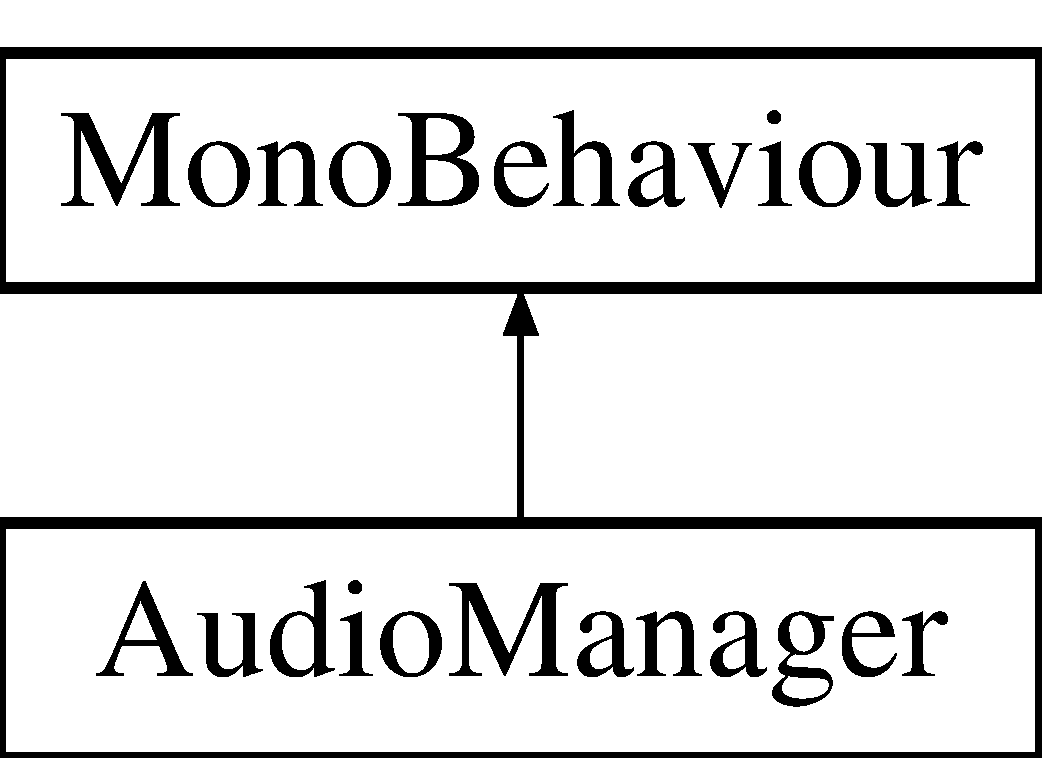
\includegraphics[height=2.000000cm]{class_audio_manager}
\end{center}
\end{figure}


\subsection{Detailed Description}
Manages the ingame sounds 



The documentation for this class was generated from the following file\+:\begin{DoxyCompactItemize}
\item 
Assets/\+Scripts/\+Managers/Audio\+Manager.\+cs\end{DoxyCompactItemize}

\hypertarget{class_background_manager}{}\section{Background\+Manager Class Reference}
\label{class_background_manager}\index{Background\+Manager@{Background\+Manager}}


Manages the ingame background and gets the correct background  


Inheritance diagram for Background\+Manager\+:\begin{figure}[H]
\begin{center}
\leavevmode
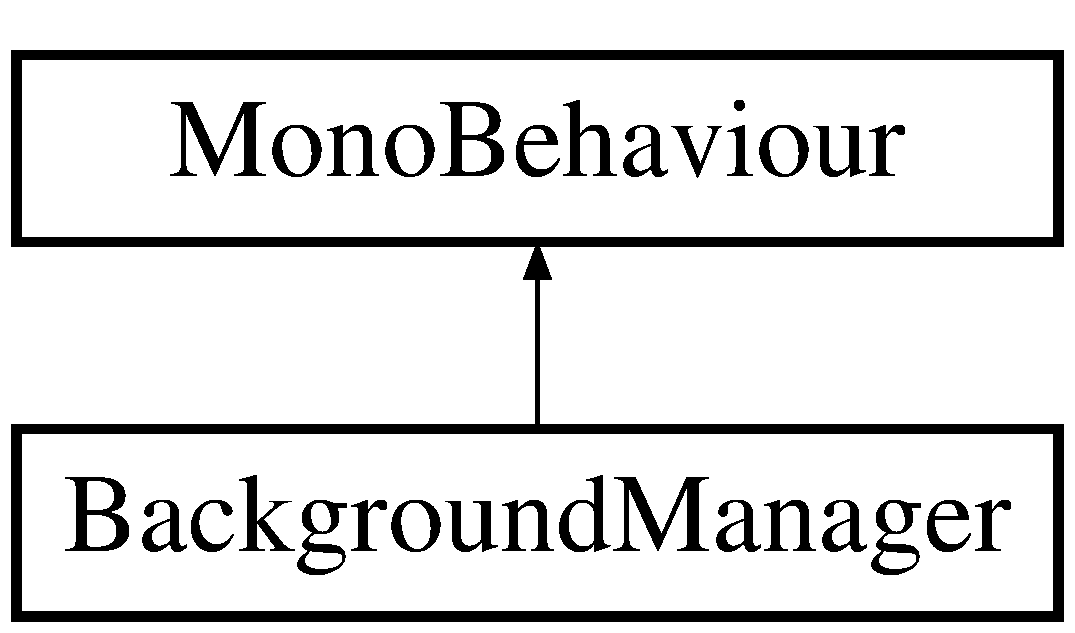
\includegraphics[height=2.000000cm]{class_background_manager}
\end{center}
\end{figure}


\subsection{Detailed Description}
Manages the ingame background and gets the correct background 



The documentation for this class was generated from the following file\+:\begin{DoxyCompactItemize}
\item 
Assets/\+Scripts/\+Managers/Background\+Manager.\+cs\end{DoxyCompactItemize}

\hypertarget{class_ball_animation_controller}{}\section{Ball\+Animation\+Controller Class Reference}
\label{class_ball_animation_controller}\index{Ball\+Animation\+Controller@{Ball\+Animation\+Controller}}
Inheritance diagram for Ball\+Animation\+Controller\+:\begin{figure}[H]
\begin{center}
\leavevmode
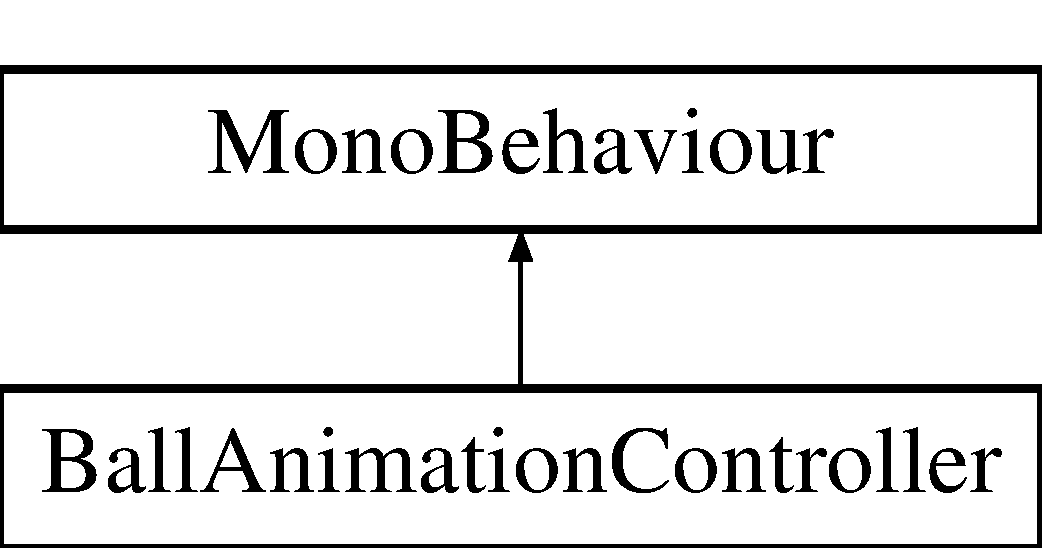
\includegraphics[height=2.000000cm]{class_ball_animation_controller}
\end{center}
\end{figure}
\subsection*{Classes}
\begin{DoxyCompactItemize}
\item 
struct \hyperlink{struct_ball_animation_controller_1_1_particle_system_struct}{Particle\+System\+Struct}
\begin{DoxyCompactList}\small\item\em Struct for particle sytems so i don\textquotesingle{}t have to repeat much code \end{DoxyCompactList}\end{DoxyCompactItemize}
\subsection*{Public Member Functions}
\begin{DoxyCompactItemize}
\item 
void {\bfseries On\+Destroy} ()\hypertarget{class_ball_animation_controller_adafe51d20a1590069256f5ed9c7145f3}{}\label{class_ball_animation_controller_adafe51d20a1590069256f5ed9c7145f3}

\item 
void \hyperlink{class_ball_animation_controller_a19beeaad6706755e27cfefe0dd289665}{setup\+Particle\+Systems} ()
\begin{DoxyCompactList}\small\item\em Init for Particle\+Systems This way it does not enable more than there are particle systems \end{DoxyCompactList}\end{DoxyCompactItemize}


\subsection{Member Function Documentation}
\index{Ball\+Animation\+Controller@{Ball\+Animation\+Controller}!setup\+Particle\+Systems@{setup\+Particle\+Systems}}
\index{setup\+Particle\+Systems@{setup\+Particle\+Systems}!Ball\+Animation\+Controller@{Ball\+Animation\+Controller}}
\subsubsection[{\texorpdfstring{setup\+Particle\+Systems()}{setupParticleSystems()}}]{\setlength{\rightskip}{0pt plus 5cm}void Ball\+Animation\+Controller.\+setup\+Particle\+Systems (
\begin{DoxyParamCaption}
{}
\end{DoxyParamCaption}
)\hspace{0.3cm}{\ttfamily [inline]}}\hypertarget{class_ball_animation_controller_a19beeaad6706755e27cfefe0dd289665}{}\label{class_ball_animation_controller_a19beeaad6706755e27cfefe0dd289665}


Init for Particle\+Systems This way it does not enable more than there are particle systems 



The documentation for this class was generated from the following file\+:\begin{DoxyCompactItemize}
\item 
Assets/\+Scripts/\+Controlers/Ball\+Animation\+Controller.\+cs\end{DoxyCompactItemize}

\hypertarget{class_ball_controller}{}\section{Ball\+Controller Class Reference}
\label{class_ball_controller}\index{Ball\+Controller@{Ball\+Controller}}
Inheritance diagram for Ball\+Controller\+:\begin{figure}[H]
\begin{center}
\leavevmode
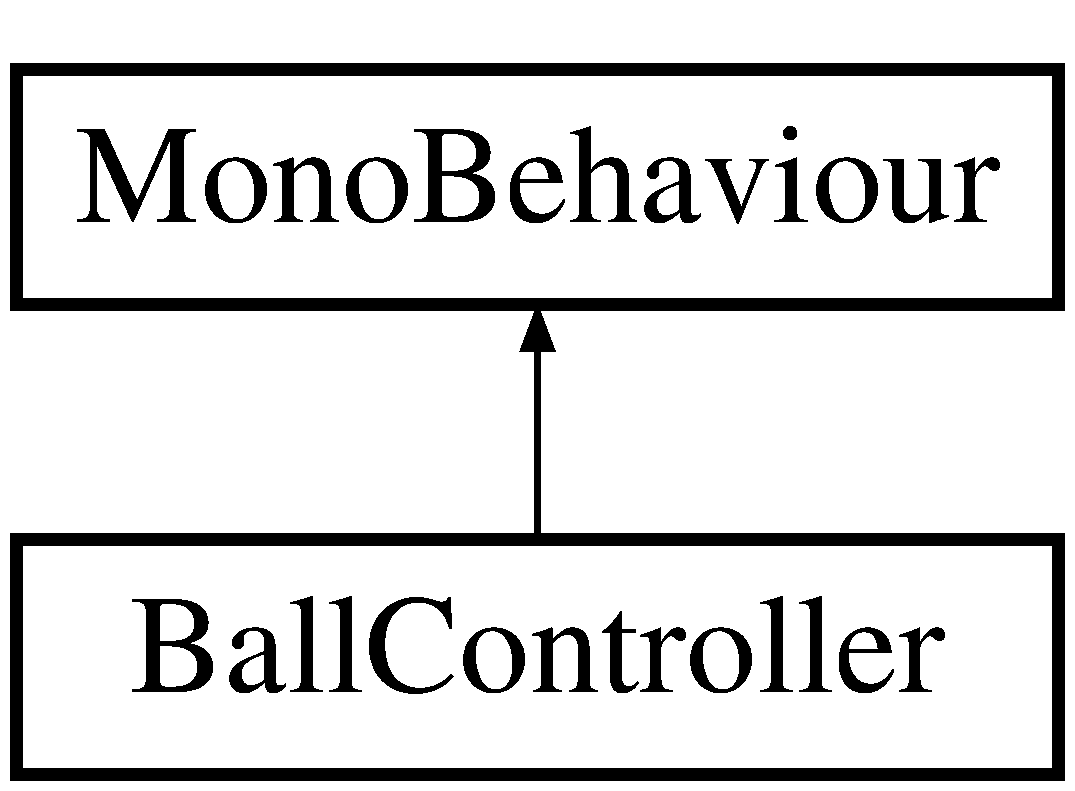
\includegraphics[height=2.000000cm]{class_ball_controller}
\end{center}
\end{figure}
\subsection*{Public Member Functions}
\begin{DoxyCompactItemize}
\item 
void \hyperlink{class_ball_controller_acb6de308cee7675f3732a48a82c6e39d}{Change\+Looks} ()
\begin{DoxyCompactList}\small\item\em Swaps sprite of the object currently Also swaps animation controler of the ball \end{DoxyCompactList}\item 
void {\bfseries On\+Destroy} ()\hypertarget{class_ball_controller_ad35c0b5aaf8fa8159b0d5c9e76f8ed11}{}\label{class_ball_controller_ad35c0b5aaf8fa8159b0d5c9e76f8ed11}

\item 
void \hyperlink{class_ball_controller_acec4d88fdeba4ef3dbd8d5c35782801f}{On\+Trigger\+Enter2D} (Collider2D collision)
\begin{DoxyCompactList}\small\item\em Unity Function \end{DoxyCompactList}\item 
void {\bfseries On\+Collision\+Enter2D} (Collision2D collision)\hypertarget{class_ball_controller_ab2fd3c261b304252ac9e39f831cf1198}{}\label{class_ball_controller_ab2fd3c261b304252ac9e39f831cf1198}

\end{DoxyCompactItemize}


\subsection{Member Function Documentation}
\index{Ball\+Controller@{Ball\+Controller}!Change\+Looks@{Change\+Looks}}
\index{Change\+Looks@{Change\+Looks}!Ball\+Controller@{Ball\+Controller}}
\subsubsection[{\texorpdfstring{Change\+Looks()}{ChangeLooks()}}]{\setlength{\rightskip}{0pt plus 5cm}void Ball\+Controller.\+Change\+Looks (
\begin{DoxyParamCaption}
{}
\end{DoxyParamCaption}
)\hspace{0.3cm}{\ttfamily [inline]}}\hypertarget{class_ball_controller_acb6de308cee7675f3732a48a82c6e39d}{}\label{class_ball_controller_acb6de308cee7675f3732a48a82c6e39d}


Swaps sprite of the object currently Also swaps animation controler of the ball 

\index{Ball\+Controller@{Ball\+Controller}!On\+Trigger\+Enter2D@{On\+Trigger\+Enter2D}}
\index{On\+Trigger\+Enter2D@{On\+Trigger\+Enter2D}!Ball\+Controller@{Ball\+Controller}}
\subsubsection[{\texorpdfstring{On\+Trigger\+Enter2\+D(\+Collider2\+D collision)}{OnTriggerEnter2D(Collider2D collision)}}]{\setlength{\rightskip}{0pt plus 5cm}void Ball\+Controller.\+On\+Trigger\+Enter2D (
\begin{DoxyParamCaption}
\item[{Collider2D}]{collision}
\end{DoxyParamCaption}
)\hspace{0.3cm}{\ttfamily [inline]}}\hypertarget{class_ball_controller_acec4d88fdeba4ef3dbd8d5c35782801f}{}\label{class_ball_controller_acec4d88fdeba4ef3dbd8d5c35782801f}


Unity Function 


\begin{DoxyParams}{Parameters}
{\em collision} & \\
\hline
\end{DoxyParams}


The documentation for this class was generated from the following file\+:\begin{DoxyCompactItemize}
\item 
Assets/\+Scripts/\+Controlers/Ball\+Controller.\+cs\end{DoxyCompactItemize}

\hypertarget{class_menus_1_1_shop_menu_data_1_1_ball_store_object}{}\section{Menus.\+Shop\+Menu\+Data.\+Ball\+Store\+Object Class Reference}
\label{class_menus_1_1_shop_menu_data_1_1_ball_store_object}\index{Menus.\+Shop\+Menu\+Data.\+Ball\+Store\+Object@{Menus.\+Shop\+Menu\+Data.\+Ball\+Store\+Object}}


A exstention of store\+Object with the added data needed for a ball object This was added so it would look quite a bit cleaner  


Inheritance diagram for Menus.\+Shop\+Menu\+Data.\+Ball\+Store\+Object\+:\begin{figure}[H]
\begin{center}
\leavevmode
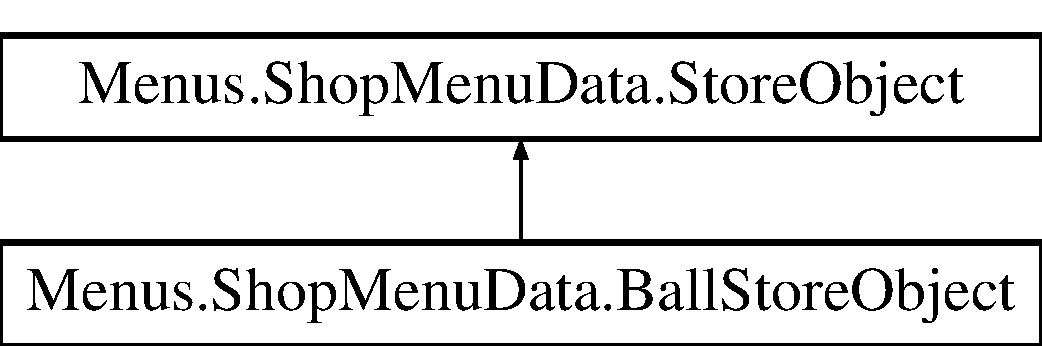
\includegraphics[height=2.000000cm]{class_menus_1_1_shop_menu_data_1_1_ball_store_object}
\end{center}
\end{figure}
\subsection*{Properties}
\begin{DoxyCompactItemize}
\item 
Material\mbox{[}$\,$\mbox{]} {\bfseries Particle\+Material}\hspace{0.3cm}{\ttfamily  \mbox{[}get\mbox{]}}\hypertarget{class_menus_1_1_shop_menu_data_1_1_ball_store_object_a3b1cba2ae730d691d4ac40d58cf9113c}{}\label{class_menus_1_1_shop_menu_data_1_1_ball_store_object_a3b1cba2ae730d691d4ac40d58cf9113c}

\item 
Runtime\+Animator\+Controller {\bfseries Animation\+Controler}\hspace{0.3cm}{\ttfamily  \mbox{[}get\mbox{]}}\hypertarget{class_menus_1_1_shop_menu_data_1_1_ball_store_object_a804f3abdad7315e197f31593bd869d12}{}\label{class_menus_1_1_shop_menu_data_1_1_ball_store_object_a804f3abdad7315e197f31593bd869d12}

\item 
Audio\+Clip {\bfseries Hit\+Sound}\hspace{0.3cm}{\ttfamily  \mbox{[}get\mbox{]}}\hypertarget{class_menus_1_1_shop_menu_data_1_1_ball_store_object_a23e8730ad4dde7894da113c90a86ebea}{}\label{class_menus_1_1_shop_menu_data_1_1_ball_store_object_a23e8730ad4dde7894da113c90a86ebea}

\item 
Audio\+Clip {\bfseries Score\+Sound}\hspace{0.3cm}{\ttfamily  \mbox{[}get\mbox{]}}\hypertarget{class_menus_1_1_shop_menu_data_1_1_ball_store_object_a350ab071bd64b096bccfedebd0005862}{}\label{class_menus_1_1_shop_menu_data_1_1_ball_store_object_a350ab071bd64b096bccfedebd0005862}

\end{DoxyCompactItemize}
\subsection*{Additional Inherited Members}


\subsection{Detailed Description}
A exstention of store\+Object with the added data needed for a ball object This was added so it would look quite a bit cleaner 



The documentation for this class was generated from the following file\+:\begin{DoxyCompactItemize}
\item 
Assets/\+Scripts/\+U\+I/\+Shop\+Menu/Shop\+Menu\+Data.\+cs\end{DoxyCompactItemize}

\hypertarget{class_menus_1_1_base_menu}{}\section{Menus.\+Base\+Menu Class Reference}
\label{class_menus_1_1_base_menu}\index{Menus.\+Base\+Menu@{Menus.\+Base\+Menu}}
Inheritance diagram for Menus.\+Base\+Menu\+:\begin{figure}[H]
\begin{center}
\leavevmode
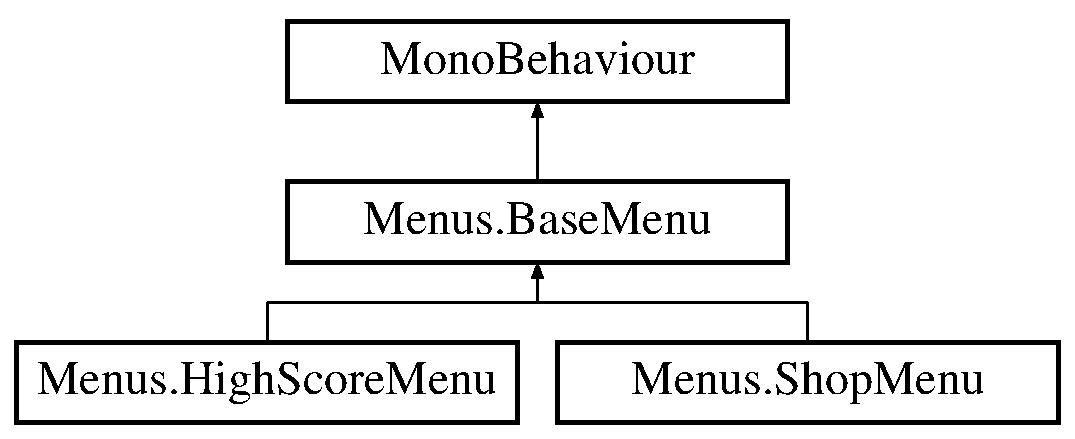
\includegraphics[height=3.000000cm]{class_menus_1_1_base_menu}
\end{center}
\end{figure}
\subsection*{Public Member Functions}
\begin{DoxyCompactItemize}
\item 
virtual void \hyperlink{class_menus_1_1_base_menu_aedf5a0abb1c46b9687cba0f216734176}{Open} ()
\begin{DoxyCompactList}\small\item\em Open menu \end{DoxyCompactList}\item 
virtual void \hyperlink{class_menus_1_1_base_menu_a9d4fb5bab4fd1c5288774cc4e1e341af}{Close} ()
\begin{DoxyCompactList}\small\item\em Closes menu \end{DoxyCompactList}\end{DoxyCompactItemize}
\subsection*{Events}
\begin{DoxyCompactItemize}
\item 
Void\+Delegate {\bfseries on\+Close}\hypertarget{class_menus_1_1_base_menu_ab6f7e2c71bb9dc828964269ebbf93685}{}\label{class_menus_1_1_base_menu_ab6f7e2c71bb9dc828964269ebbf93685}

\end{DoxyCompactItemize}


\subsection{Member Function Documentation}
\index{Menus\+::\+Base\+Menu@{Menus\+::\+Base\+Menu}!Close@{Close}}
\index{Close@{Close}!Menus\+::\+Base\+Menu@{Menus\+::\+Base\+Menu}}
\subsubsection[{\texorpdfstring{Close()}{Close()}}]{\setlength{\rightskip}{0pt plus 5cm}virtual void Menus.\+Base\+Menu.\+Close (
\begin{DoxyParamCaption}
{}
\end{DoxyParamCaption}
)\hspace{0.3cm}{\ttfamily [inline]}, {\ttfamily [virtual]}}\hypertarget{class_menus_1_1_base_menu_a9d4fb5bab4fd1c5288774cc4e1e341af}{}\label{class_menus_1_1_base_menu_a9d4fb5bab4fd1c5288774cc4e1e341af}


Closes menu 

by default it sends a event when the menu is closed the menu is closed by disabling the game object \index{Menus\+::\+Base\+Menu@{Menus\+::\+Base\+Menu}!Open@{Open}}
\index{Open@{Open}!Menus\+::\+Base\+Menu@{Menus\+::\+Base\+Menu}}
\subsubsection[{\texorpdfstring{Open()}{Open()}}]{\setlength{\rightskip}{0pt plus 5cm}virtual void Menus.\+Base\+Menu.\+Open (
\begin{DoxyParamCaption}
{}
\end{DoxyParamCaption}
)\hspace{0.3cm}{\ttfamily [inline]}, {\ttfamily [virtual]}}\hypertarget{class_menus_1_1_base_menu_aedf5a0abb1c46b9687cba0f216734176}{}\label{class_menus_1_1_base_menu_aedf5a0abb1c46b9687cba0f216734176}


Open menu 

by default it just enables and disables the game object 

Reimplemented in \hyperlink{class_menus_1_1_shop_menu_af79b153c30d06137091f0b021d2c626b}{Menus.\+Shop\+Menu}.



The documentation for this class was generated from the following file\+:\begin{DoxyCompactItemize}
\item 
Assets/\+Scripts/\+U\+I/Base\+Menu.\+cs\end{DoxyCompactItemize}

\hypertarget{class_custom_grid}{}\section{Custom\+Grid Class Reference}
\label{class_custom_grid}\index{Custom\+Grid@{Custom\+Grid}}


A grid sorting method that has the abilty create simple soothend animations. It also only does things when it detects changes making it quite light;  


Inheritance diagram for Custom\+Grid\+:\begin{figure}[H]
\begin{center}
\leavevmode
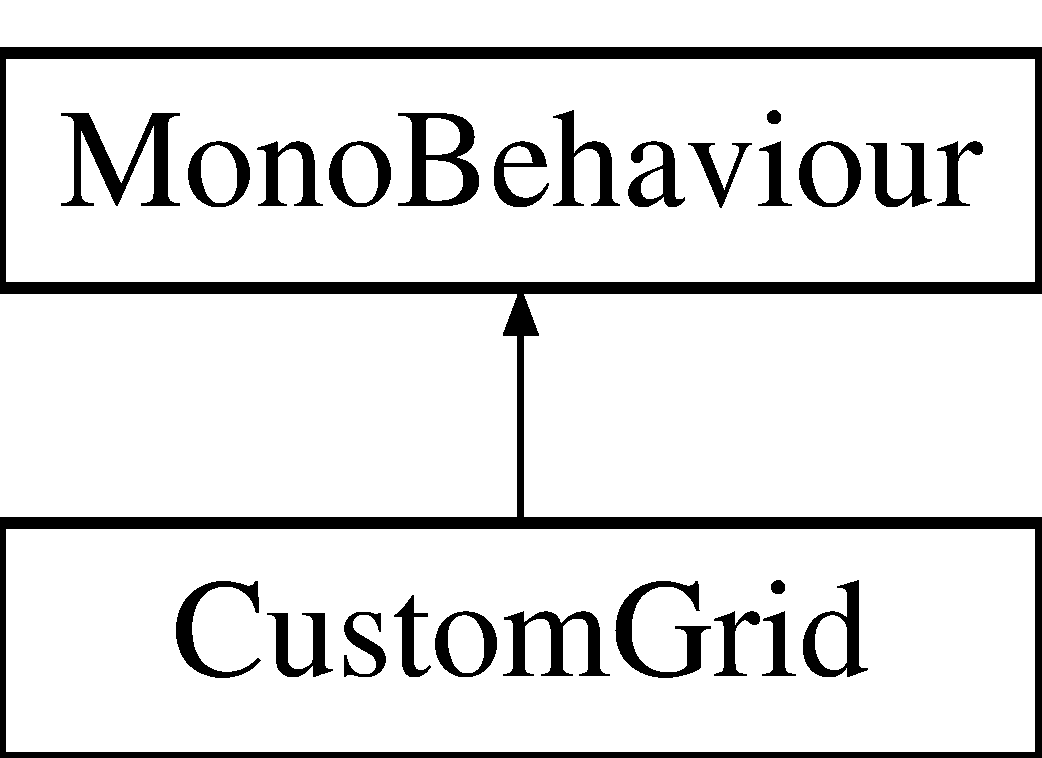
\includegraphics[height=2.000000cm]{class_custom_grid}
\end{center}
\end{figure}
\subsection*{Public Member Functions}
\begin{DoxyCompactItemize}
\item 
void \hyperlink{class_custom_grid_a1b2b4541146de94aaead99bca2f78d7f}{Force\+Update} ()
\begin{DoxyCompactList}\small\item\em Used for force call a update \end{DoxyCompactList}\end{DoxyCompactItemize}
\subsection*{Public Attributes}
\begin{DoxyCompactItemize}
\item 
Vector2 \hyperlink{class_custom_grid_a0cf591b7ae82c985d1983171d9391712}{Obj\+Size}
\begin{DoxyCompactList}\small\item\em Size that each object will have \end{DoxyCompactList}\item 
Vector2 \hyperlink{class_custom_grid_aa1f53f156756dfe4d9d2795fe2c52754}{padding}
\begin{DoxyCompactList}\small\item\em forced space between each object \end{DoxyCompactList}\item 
Vector2 \hyperlink{class_custom_grid_a068ef9a666cd31142751320e2a653025}{max\+Spacing}
\begin{DoxyCompactList}\small\item\em the maxium space between two objects \end{DoxyCompactList}\item 
Vector2 \hyperlink{class_custom_grid_af7596d0b65aa5ea01ae27898c523b1b5}{Anchor\+Point} = Vector2.\+zero
\begin{DoxyCompactList}\small\item\em The anchor point or from wich the object wil be centered \end{DoxyCompactList}\item 
Vector2 \hyperlink{class_custom_grid_ab9594c84442d7bd9f8cad31cd2d75c84}{Current\+Spacing} = Vector2.\+zero
\begin{DoxyCompactList}\small\item\em The current space between the objects \end{DoxyCompactList}\item 
int \hyperlink{class_custom_grid_a74432277987a0e6cc02d0db891ec77ba}{max\+Rows} = 2
\begin{DoxyCompactList}\small\item\em The maxium number of rows \end{DoxyCompactList}\item 
int \hyperlink{class_custom_grid_a985fc1fc02418d3286ffbd41c98417a5}{min\+Needed\+For\+First\+Row} = 2
\begin{DoxyCompactList}\small\item\em The minum objecs on a single row needed before it creates a second row \end{DoxyCompactList}\item 
float \hyperlink{class_custom_grid_aa07b1f547bdbef9d050b5f57d96f744a}{yoffset}
\begin{DoxyCompactList}\small\item\em The y offset used for when the objects are not well centered them selfs \end{DoxyCompactList}\item 
bool \hyperlink{class_custom_grid_a9bddd45525d796a4db2edcbe8f669773}{continues\+Updates} = false
\begin{DoxyCompactList}\small\item\em Does the grid update continuesly. usefull when debugging the grid or seeing if everything works correctly. Recommened to have it turned of when you are building the game because it saves preformance \end{DoxyCompactList}\item 
bool \hyperlink{class_custom_grid_ae7281905d1114c2582f02d0d1badf53f}{use\+Animations} = false
\begin{DoxyCompactList}\small\item\em Enable the animations so that the elements move towards the new points instead of teleporting \end{DoxyCompactList}\end{DoxyCompactItemize}


\subsection{Detailed Description}
A grid sorting method that has the abilty create simple soothend animations. It also only does things when it detects changes making it quite light; 



\subsection{Member Function Documentation}
\index{Custom\+Grid@{Custom\+Grid}!Force\+Update@{Force\+Update}}
\index{Force\+Update@{Force\+Update}!Custom\+Grid@{Custom\+Grid}}
\subsubsection[{\texorpdfstring{Force\+Update()}{ForceUpdate()}}]{\setlength{\rightskip}{0pt plus 5cm}void Custom\+Grid.\+Force\+Update (
\begin{DoxyParamCaption}
{}
\end{DoxyParamCaption}
)\hspace{0.3cm}{\ttfamily [inline]}}\hypertarget{class_custom_grid_a1b2b4541146de94aaead99bca2f78d7f}{}\label{class_custom_grid_a1b2b4541146de94aaead99bca2f78d7f}


Used for force call a update 



\subsection{Member Data Documentation}
\index{Custom\+Grid@{Custom\+Grid}!Anchor\+Point@{Anchor\+Point}}
\index{Anchor\+Point@{Anchor\+Point}!Custom\+Grid@{Custom\+Grid}}
\subsubsection[{\texorpdfstring{Anchor\+Point}{AnchorPoint}}]{\setlength{\rightskip}{0pt plus 5cm}Vector2 Custom\+Grid.\+Anchor\+Point = Vector2.\+zero}\hypertarget{class_custom_grid_af7596d0b65aa5ea01ae27898c523b1b5}{}\label{class_custom_grid_af7596d0b65aa5ea01ae27898c523b1b5}


The anchor point or from wich the object wil be centered 

\index{Custom\+Grid@{Custom\+Grid}!continues\+Updates@{continues\+Updates}}
\index{continues\+Updates@{continues\+Updates}!Custom\+Grid@{Custom\+Grid}}
\subsubsection[{\texorpdfstring{continues\+Updates}{continuesUpdates}}]{\setlength{\rightskip}{0pt plus 5cm}bool Custom\+Grid.\+continues\+Updates = false}\hypertarget{class_custom_grid_a9bddd45525d796a4db2edcbe8f669773}{}\label{class_custom_grid_a9bddd45525d796a4db2edcbe8f669773}


Does the grid update continuesly. usefull when debugging the grid or seeing if everything works correctly. Recommened to have it turned of when you are building the game because it saves preformance 

\index{Custom\+Grid@{Custom\+Grid}!Current\+Spacing@{Current\+Spacing}}
\index{Current\+Spacing@{Current\+Spacing}!Custom\+Grid@{Custom\+Grid}}
\subsubsection[{\texorpdfstring{Current\+Spacing}{CurrentSpacing}}]{\setlength{\rightskip}{0pt plus 5cm}Vector2 Custom\+Grid.\+Current\+Spacing = Vector2.\+zero}\hypertarget{class_custom_grid_ab9594c84442d7bd9f8cad31cd2d75c84}{}\label{class_custom_grid_ab9594c84442d7bd9f8cad31cd2d75c84}


The current space between the objects 

\index{Custom\+Grid@{Custom\+Grid}!max\+Rows@{max\+Rows}}
\index{max\+Rows@{max\+Rows}!Custom\+Grid@{Custom\+Grid}}
\subsubsection[{\texorpdfstring{max\+Rows}{maxRows}}]{\setlength{\rightskip}{0pt plus 5cm}int Custom\+Grid.\+max\+Rows = 2}\hypertarget{class_custom_grid_a74432277987a0e6cc02d0db891ec77ba}{}\label{class_custom_grid_a74432277987a0e6cc02d0db891ec77ba}


The maxium number of rows 

\index{Custom\+Grid@{Custom\+Grid}!max\+Spacing@{max\+Spacing}}
\index{max\+Spacing@{max\+Spacing}!Custom\+Grid@{Custom\+Grid}}
\subsubsection[{\texorpdfstring{max\+Spacing}{maxSpacing}}]{\setlength{\rightskip}{0pt plus 5cm}Vector2 Custom\+Grid.\+max\+Spacing}\hypertarget{class_custom_grid_a068ef9a666cd31142751320e2a653025}{}\label{class_custom_grid_a068ef9a666cd31142751320e2a653025}


the maxium space between two objects 

\index{Custom\+Grid@{Custom\+Grid}!min\+Needed\+For\+First\+Row@{min\+Needed\+For\+First\+Row}}
\index{min\+Needed\+For\+First\+Row@{min\+Needed\+For\+First\+Row}!Custom\+Grid@{Custom\+Grid}}
\subsubsection[{\texorpdfstring{min\+Needed\+For\+First\+Row}{minNeededForFirstRow}}]{\setlength{\rightskip}{0pt plus 5cm}int Custom\+Grid.\+min\+Needed\+For\+First\+Row = 2}\hypertarget{class_custom_grid_a985fc1fc02418d3286ffbd41c98417a5}{}\label{class_custom_grid_a985fc1fc02418d3286ffbd41c98417a5}


The minum objecs on a single row needed before it creates a second row 

\index{Custom\+Grid@{Custom\+Grid}!Obj\+Size@{Obj\+Size}}
\index{Obj\+Size@{Obj\+Size}!Custom\+Grid@{Custom\+Grid}}
\subsubsection[{\texorpdfstring{Obj\+Size}{ObjSize}}]{\setlength{\rightskip}{0pt plus 5cm}Vector2 Custom\+Grid.\+Obj\+Size}\hypertarget{class_custom_grid_a0cf591b7ae82c985d1983171d9391712}{}\label{class_custom_grid_a0cf591b7ae82c985d1983171d9391712}


Size that each object will have 

\index{Custom\+Grid@{Custom\+Grid}!padding@{padding}}
\index{padding@{padding}!Custom\+Grid@{Custom\+Grid}}
\subsubsection[{\texorpdfstring{padding}{padding}}]{\setlength{\rightskip}{0pt plus 5cm}Vector2 Custom\+Grid.\+padding}\hypertarget{class_custom_grid_aa1f53f156756dfe4d9d2795fe2c52754}{}\label{class_custom_grid_aa1f53f156756dfe4d9d2795fe2c52754}


forced space between each object 

\index{Custom\+Grid@{Custom\+Grid}!use\+Animations@{use\+Animations}}
\index{use\+Animations@{use\+Animations}!Custom\+Grid@{Custom\+Grid}}
\subsubsection[{\texorpdfstring{use\+Animations}{useAnimations}}]{\setlength{\rightskip}{0pt plus 5cm}bool Custom\+Grid.\+use\+Animations = false}\hypertarget{class_custom_grid_ae7281905d1114c2582f02d0d1badf53f}{}\label{class_custom_grid_ae7281905d1114c2582f02d0d1badf53f}


Enable the animations so that the elements move towards the new points instead of teleporting 

\index{Custom\+Grid@{Custom\+Grid}!yoffset@{yoffset}}
\index{yoffset@{yoffset}!Custom\+Grid@{Custom\+Grid}}
\subsubsection[{\texorpdfstring{yoffset}{yoffset}}]{\setlength{\rightskip}{0pt plus 5cm}float Custom\+Grid.\+yoffset}\hypertarget{class_custom_grid_aa07b1f547bdbef9d050b5f57d96f744a}{}\label{class_custom_grid_aa07b1f547bdbef9d050b5f57d96f744a}


The y offset used for when the objects are not well centered them selfs 



The documentation for this class was generated from the following file\+:\begin{DoxyCompactItemize}
\item 
Assets/\+Scripts/\+Util/Custom\+Grid.\+cs\end{DoxyCompactItemize}

\hypertarget{class_events_1_1_event_dispatcher}{}\section{Events.\+Event\+Dispatcher Class Reference}
\label{class_events_1_1_event_dispatcher}\index{Events.\+Event\+Dispatcher@{Events.\+Event\+Dispatcher}}


Event dispatcher class.  


Inheritance diagram for Events.\+Event\+Dispatcher\+:\begin{figure}[H]
\begin{center}
\leavevmode
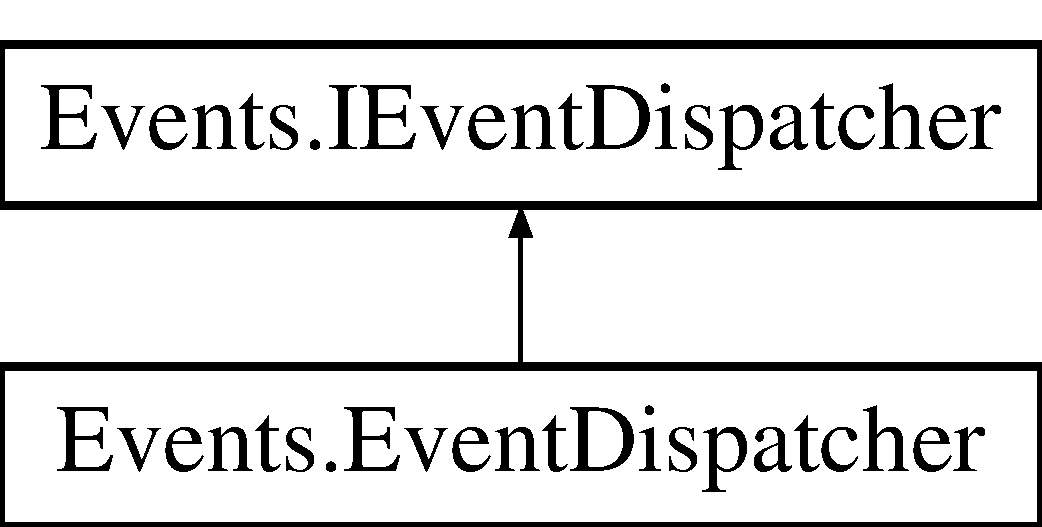
\includegraphics[height=2.000000cm]{class_events_1_1_event_dispatcher}
\end{center}
\end{figure}
\subsection*{Public Member Functions}
\begin{DoxyCompactItemize}
\item 
void \hyperlink{class_events_1_1_event_dispatcher_af8047b3f53861d56c27aa02e358486a2}{Add\+Event\+Listener} (Type type, Action handler)
\begin{DoxyCompactList}\small\item\em Implementation of \hyperlink{interface_events_1_1_i_event_dispatcher_ac22d58973ca79fdaea1471704dba0e01}{I\+Event\+Dispatcher.\+Add\+Event\+Listener(\+Type, Action)} \end{DoxyCompactList}\item 
void \hyperlink{class_events_1_1_event_dispatcher_ab90178e5a5bbfd90601347ab8489cf01}{Add\+Event\+Listener$<$ T $>$} (Action$<$ T $>$ handler)
\begin{DoxyCompactList}\small\item\em Imprementation of \hyperlink{interface_events_1_1_i_event_dispatcher_a4c10e52a26a0c354bcaae21e0a240f93}{I\+Event\+Dispatcher.\+Add\+Event\+Listener$<$\+T$>$(\+Action$<$\+T$>$)} \end{DoxyCompactList}\item 
void \hyperlink{class_events_1_1_event_dispatcher_a9644ebc4fb5655cda345b586e5749ea0}{Remove\+Event\+Listener} (Type type, Action handler)
\begin{DoxyCompactList}\small\item\em Implementation of \hyperlink{interface_events_1_1_i_event_dispatcher_ae3209681ebdbcf8289905ff6ccdbd188}{I\+Event\+Dispatcher.\+Remove\+Event\+Listener(\+Type, Action)} \end{DoxyCompactList}\item 
void \hyperlink{class_events_1_1_event_dispatcher_a88f24cbfab1022517830b3fc42155c15}{Remove\+Event\+Listener$<$ T $>$} (Action$<$ T $>$ handler)
\begin{DoxyCompactList}\small\item\em Implementation of \hyperlink{interface_events_1_1_i_event_dispatcher_a86e3438c779746108c3f01dff0c43d23}{I\+Event\+Dispatcher.\+Remove\+Event\+Listener$<$\+T$>$(\+Action$<$\+T$>$)} \end{DoxyCompactList}\item 
void \hyperlink{class_events_1_1_event_dispatcher_add2667245c85f8d781eed8d908450518}{Remove\+All\+Listeners} ()
\begin{DoxyCompactList}\small\item\em Remove all registered Listeners. \end{DoxyCompactList}\item 
void \hyperlink{class_events_1_1_event_dispatcher_a4bec3274dceea156c52248cac71e968c}{Invoke} (Type type, object evt)
\begin{DoxyCompactList}\small\item\em Implementation of \hyperlink{interface_events_1_1_i_event_dispatcher_a3789c396884e0097a4efdd8fb6652214}{I\+Event\+Dispatcher.\+Invoke(\+Type, object)} \end{DoxyCompactList}\item 
void \hyperlink{class_events_1_1_event_dispatcher_a7c1fe1b9738ea149420d19c1131f2f25}{Invoke$<$ T $>$} (T evt)
\begin{DoxyCompactList}\small\item\em Implementation of \hyperlink{interface_events_1_1_i_event_dispatcher_ab6e50172a6c4a5ec91977f183278dc91}{I\+Event\+Dispatcher.\+Invoke$<$\+T$>$(\+T)} \end{DoxyCompactList}\end{DoxyCompactItemize}


\subsection{Detailed Description}
Event dispatcher class. 



\subsection{Member Function Documentation}
\index{Events\+::\+Event\+Dispatcher@{Events\+::\+Event\+Dispatcher}!Add\+Event\+Listener@{Add\+Event\+Listener}}
\index{Add\+Event\+Listener@{Add\+Event\+Listener}!Events\+::\+Event\+Dispatcher@{Events\+::\+Event\+Dispatcher}}
\subsubsection[{\texorpdfstring{Add\+Event\+Listener(\+Type type, Action handler)}{AddEventListener(Type type, Action handler)}}]{\setlength{\rightskip}{0pt plus 5cm}void Events.\+Event\+Dispatcher.\+Add\+Event\+Listener (
\begin{DoxyParamCaption}
\item[{Type}]{type, }
\item[{Action}]{handler}
\end{DoxyParamCaption}
)\hspace{0.3cm}{\ttfamily [inline]}}\hypertarget{class_events_1_1_event_dispatcher_af8047b3f53861d56c27aa02e358486a2}{}\label{class_events_1_1_event_dispatcher_af8047b3f53861d56c27aa02e358486a2}


Implementation of \hyperlink{interface_events_1_1_i_event_dispatcher_ac22d58973ca79fdaea1471704dba0e01}{I\+Event\+Dispatcher.\+Add\+Event\+Listener(\+Type, Action)} 


\begin{DoxyParams}{Parameters}
{\em type} & The type of event to be added.\\
\hline
{\em handler} & The handler.\\
\hline
\end{DoxyParams}


Implements \hyperlink{interface_events_1_1_i_event_dispatcher_ac22d58973ca79fdaea1471704dba0e01}{Events.\+I\+Event\+Dispatcher}.

\index{Events\+::\+Event\+Dispatcher@{Events\+::\+Event\+Dispatcher}!Add\+Event\+Listener$<$ T $>$@{Add\+Event\+Listener$<$ T $>$}}
\index{Add\+Event\+Listener$<$ T $>$@{Add\+Event\+Listener$<$ T $>$}!Events\+::\+Event\+Dispatcher@{Events\+::\+Event\+Dispatcher}}
\subsubsection[{\texorpdfstring{Add\+Event\+Listener$<$ T $>$(\+Action$<$ T $>$ handler)}{AddEventListener< T >(Action< T > handler)}}]{\setlength{\rightskip}{0pt plus 5cm}void {\bf Events.\+Event\+Dispatcher.\+Add\+Event\+Listener}$<$ T $>$ (
\begin{DoxyParamCaption}
\item[{Action$<$ T $>$}]{handler}
\end{DoxyParamCaption}
)\hspace{0.3cm}{\ttfamily [inline]}}\hypertarget{class_events_1_1_event_dispatcher_ab90178e5a5bbfd90601347ab8489cf01}{}\label{class_events_1_1_event_dispatcher_ab90178e5a5bbfd90601347ab8489cf01}


Imprementation of \hyperlink{interface_events_1_1_i_event_dispatcher_a4c10e52a26a0c354bcaae21e0a240f93}{I\+Event\+Dispatcher.\+Add\+Event\+Listener$<$\+T$>$(\+Action$<$\+T$>$)} 


\begin{DoxyTemplParams}{Template Parameters}
{\em T} & The type of event to be added.\\
\hline
\end{DoxyTemplParams}

\begin{DoxyParams}{Parameters}
{\em handler} & The handler.\\
\hline
\end{DoxyParams}


Implements \hyperlink{interface_events_1_1_i_event_dispatcher_a4c10e52a26a0c354bcaae21e0a240f93}{Events.\+I\+Event\+Dispatcher}.

\begin{Desc}
\item[Type Constraints]\begin{description}
\item[{\em T} : {\em I\+Event}]\end{description}
\end{Desc}
\index{Events\+::\+Event\+Dispatcher@{Events\+::\+Event\+Dispatcher}!Invoke@{Invoke}}
\index{Invoke@{Invoke}!Events\+::\+Event\+Dispatcher@{Events\+::\+Event\+Dispatcher}}
\subsubsection[{\texorpdfstring{Invoke(\+Type type, object evt)}{Invoke(Type type, object evt)}}]{\setlength{\rightskip}{0pt plus 5cm}void Events.\+Event\+Dispatcher.\+Invoke (
\begin{DoxyParamCaption}
\item[{Type}]{type, }
\item[{object}]{evt}
\end{DoxyParamCaption}
)\hspace{0.3cm}{\ttfamily [inline]}}\hypertarget{class_events_1_1_event_dispatcher_a4bec3274dceea156c52248cac71e968c}{}\label{class_events_1_1_event_dispatcher_a4bec3274dceea156c52248cac71e968c}


Implementation of \hyperlink{interface_events_1_1_i_event_dispatcher_a3789c396884e0097a4efdd8fb6652214}{I\+Event\+Dispatcher.\+Invoke(\+Type, object)} 


\begin{DoxyParams}{Parameters}
{\em type} & Type of event to be evoked.\\
\hline
{\em evt} & The event to be evoked.\\
\hline
\end{DoxyParams}


Implements \hyperlink{interface_events_1_1_i_event_dispatcher_a3789c396884e0097a4efdd8fb6652214}{Events.\+I\+Event\+Dispatcher}.

\index{Events\+::\+Event\+Dispatcher@{Events\+::\+Event\+Dispatcher}!Invoke$<$ T $>$@{Invoke$<$ T $>$}}
\index{Invoke$<$ T $>$@{Invoke$<$ T $>$}!Events\+::\+Event\+Dispatcher@{Events\+::\+Event\+Dispatcher}}
\subsubsection[{\texorpdfstring{Invoke$<$ T $>$(\+T evt)}{Invoke< T >(T evt)}}]{\setlength{\rightskip}{0pt plus 5cm}void {\bf Events.\+Event\+Dispatcher.\+Invoke}$<$ T $>$ (
\begin{DoxyParamCaption}
\item[{T}]{evt}
\end{DoxyParamCaption}
)\hspace{0.3cm}{\ttfamily [inline]}}\hypertarget{class_events_1_1_event_dispatcher_a7c1fe1b9738ea149420d19c1131f2f25}{}\label{class_events_1_1_event_dispatcher_a7c1fe1b9738ea149420d19c1131f2f25}


Implementation of \hyperlink{interface_events_1_1_i_event_dispatcher_ab6e50172a6c4a5ec91977f183278dc91}{I\+Event\+Dispatcher.\+Invoke$<$\+T$>$(\+T)} 


\begin{DoxyTemplParams}{Template Parameters}
{\em T} & Type of event to be evoked.\\
\hline
\end{DoxyTemplParams}

\begin{DoxyParams}{Parameters}
{\em evt} & The event to be evoked.\\
\hline
\end{DoxyParams}


Implements \hyperlink{interface_events_1_1_i_event_dispatcher_ab6e50172a6c4a5ec91977f183278dc91}{Events.\+I\+Event\+Dispatcher}.

\begin{Desc}
\item[Type Constraints]\begin{description}
\item[{\em T} : {\em I\+Event}]\end{description}
\end{Desc}
\index{Events\+::\+Event\+Dispatcher@{Events\+::\+Event\+Dispatcher}!Remove\+All\+Listeners@{Remove\+All\+Listeners}}
\index{Remove\+All\+Listeners@{Remove\+All\+Listeners}!Events\+::\+Event\+Dispatcher@{Events\+::\+Event\+Dispatcher}}
\subsubsection[{\texorpdfstring{Remove\+All\+Listeners()}{RemoveAllListeners()}}]{\setlength{\rightskip}{0pt plus 5cm}void Events.\+Event\+Dispatcher.\+Remove\+All\+Listeners (
\begin{DoxyParamCaption}
{}
\end{DoxyParamCaption}
)\hspace{0.3cm}{\ttfamily [inline]}}\hypertarget{class_events_1_1_event_dispatcher_add2667245c85f8d781eed8d908450518}{}\label{class_events_1_1_event_dispatcher_add2667245c85f8d781eed8d908450518}


Remove all registered Listeners. 

\index{Events\+::\+Event\+Dispatcher@{Events\+::\+Event\+Dispatcher}!Remove\+Event\+Listener@{Remove\+Event\+Listener}}
\index{Remove\+Event\+Listener@{Remove\+Event\+Listener}!Events\+::\+Event\+Dispatcher@{Events\+::\+Event\+Dispatcher}}
\subsubsection[{\texorpdfstring{Remove\+Event\+Listener(\+Type type, Action handler)}{RemoveEventListener(Type type, Action handler)}}]{\setlength{\rightskip}{0pt plus 5cm}void Events.\+Event\+Dispatcher.\+Remove\+Event\+Listener (
\begin{DoxyParamCaption}
\item[{Type}]{type, }
\item[{Action}]{handler}
\end{DoxyParamCaption}
)\hspace{0.3cm}{\ttfamily [inline]}}\hypertarget{class_events_1_1_event_dispatcher_a9644ebc4fb5655cda345b586e5749ea0}{}\label{class_events_1_1_event_dispatcher_a9644ebc4fb5655cda345b586e5749ea0}


Implementation of \hyperlink{interface_events_1_1_i_event_dispatcher_ae3209681ebdbcf8289905ff6ccdbd188}{I\+Event\+Dispatcher.\+Remove\+Event\+Listener(\+Type, Action)} 


\begin{DoxyParams}{Parameters}
{\em type} & The type of event to be removed.\\
\hline
{\em handler} & The handler.\\
\hline
\end{DoxyParams}


Implements \hyperlink{interface_events_1_1_i_event_dispatcher_ae3209681ebdbcf8289905ff6ccdbd188}{Events.\+I\+Event\+Dispatcher}.

\index{Events\+::\+Event\+Dispatcher@{Events\+::\+Event\+Dispatcher}!Remove\+Event\+Listener$<$ T $>$@{Remove\+Event\+Listener$<$ T $>$}}
\index{Remove\+Event\+Listener$<$ T $>$@{Remove\+Event\+Listener$<$ T $>$}!Events\+::\+Event\+Dispatcher@{Events\+::\+Event\+Dispatcher}}
\subsubsection[{\texorpdfstring{Remove\+Event\+Listener$<$ T $>$(\+Action$<$ T $>$ handler)}{RemoveEventListener< T >(Action< T > handler)}}]{\setlength{\rightskip}{0pt plus 5cm}void {\bf Events.\+Event\+Dispatcher.\+Remove\+Event\+Listener}$<$ T $>$ (
\begin{DoxyParamCaption}
\item[{Action$<$ T $>$}]{handler}
\end{DoxyParamCaption}
)\hspace{0.3cm}{\ttfamily [inline]}}\hypertarget{class_events_1_1_event_dispatcher_a88f24cbfab1022517830b3fc42155c15}{}\label{class_events_1_1_event_dispatcher_a88f24cbfab1022517830b3fc42155c15}


Implementation of \hyperlink{interface_events_1_1_i_event_dispatcher_a86e3438c779746108c3f01dff0c43d23}{I\+Event\+Dispatcher.\+Remove\+Event\+Listener$<$\+T$>$(\+Action$<$\+T$>$)} 


\begin{DoxyTemplParams}{Template Parameters}
{\em T} & The type of event to be removed.\\
\hline
\end{DoxyTemplParams}

\begin{DoxyParams}{Parameters}
{\em handler} & The handler.\\
\hline
\end{DoxyParams}


Implements \hyperlink{interface_events_1_1_i_event_dispatcher_a86e3438c779746108c3f01dff0c43d23}{Events.\+I\+Event\+Dispatcher}.

\begin{Desc}
\item[Type Constraints]\begin{description}
\item[{\em T} : {\em I\+Event}]\end{description}
\end{Desc}


The documentation for this class was generated from the following file\+:\begin{DoxyCompactItemize}
\item 
Assets/\+Scripts/\+Util/\+Events/Event\+Dispatcher.\+cs\end{DoxyCompactItemize}

\hypertarget{class_game_manager}{}\section{Game\+Manager Class Reference}
\label{class_game_manager}\index{Game\+Manager@{Game\+Manager}}
Inheritance diagram for Game\+Manager\+:\begin{figure}[H]
\begin{center}
\leavevmode
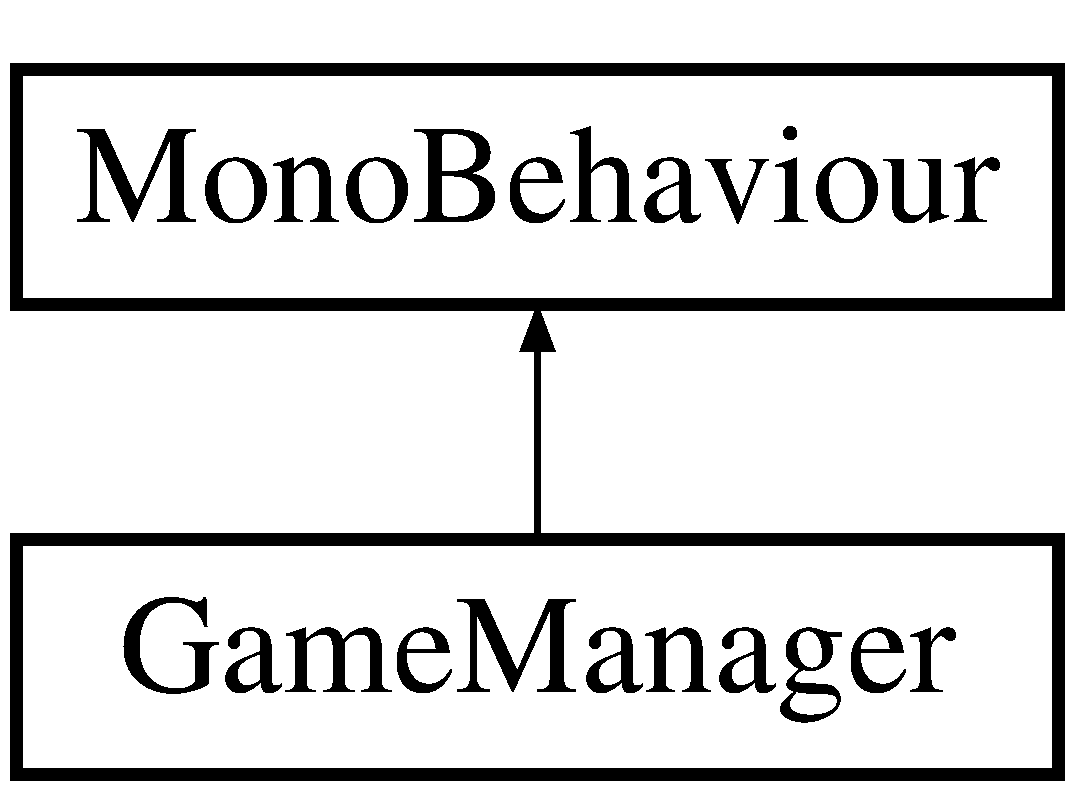
\includegraphics[height=2.000000cm]{class_game_manager}
\end{center}
\end{figure}
\subsection*{Public Member Functions}
\begin{DoxyCompactItemize}
\item 
void {\bfseries On\+Destroy} ()\hypertarget{class_game_manager_a246f3c0e365f4eff658e779f4336a4fa}{}\label{class_game_manager_a246f3c0e365f4eff658e779f4336a4fa}

\item 
void \hyperlink{class_game_manager_a2ba50fa10e943f9d7f70ca36ab162742}{Continue\+Game} ()
\begin{DoxyCompactList}\small\item\em Call to unpause game \end{DoxyCompactList}\item 
void \hyperlink{class_game_manager_adb110a6ef474e4ac7901176c97a859ab}{Pause\+Game} ()
\begin{DoxyCompactList}\small\item\em Call to pause game \end{DoxyCompactList}\end{DoxyCompactItemize}
\subsection*{Properties}
\begin{DoxyCompactItemize}
\item 
static int \hyperlink{class_game_manager_a77a552c74394d1e18c0bb2893bd27cb0}{Score}\hspace{0.3cm}{\ttfamily  \mbox{[}get\mbox{]}}
\begin{DoxyCompactList}\small\item\em The Points earned of the player \end{DoxyCompactList}\item 
static bool \hyperlink{class_game_manager_a9a7aa34c324c433dd80fa0d7d1bf37e8}{Game\+Paused}\hspace{0.3cm}{\ttfamily  \mbox{[}get\mbox{]}}
\begin{DoxyCompactList}\small\item\em Show that game is paused \end{DoxyCompactList}\end{DoxyCompactItemize}
\subsection*{Events}
\begin{DoxyCompactItemize}
\item 
static Void\+Delegate {\bfseries On\+Score\+Update}\hypertarget{class_game_manager_a9fe5549be887be90d339b7d65ad1200a}{}\label{class_game_manager_a9fe5549be887be90d339b7d65ad1200a}

\end{DoxyCompactItemize}


\subsection{Member Function Documentation}
\index{Game\+Manager@{Game\+Manager}!Continue\+Game@{Continue\+Game}}
\index{Continue\+Game@{Continue\+Game}!Game\+Manager@{Game\+Manager}}
\subsubsection[{\texorpdfstring{Continue\+Game()}{ContinueGame()}}]{\setlength{\rightskip}{0pt plus 5cm}void Game\+Manager.\+Continue\+Game (
\begin{DoxyParamCaption}
{}
\end{DoxyParamCaption}
)\hspace{0.3cm}{\ttfamily [inline]}}\hypertarget{class_game_manager_a2ba50fa10e943f9d7f70ca36ab162742}{}\label{class_game_manager_a2ba50fa10e943f9d7f70ca36ab162742}


Call to unpause game 

\index{Game\+Manager@{Game\+Manager}!Pause\+Game@{Pause\+Game}}
\index{Pause\+Game@{Pause\+Game}!Game\+Manager@{Game\+Manager}}
\subsubsection[{\texorpdfstring{Pause\+Game()}{PauseGame()}}]{\setlength{\rightskip}{0pt plus 5cm}void Game\+Manager.\+Pause\+Game (
\begin{DoxyParamCaption}
{}
\end{DoxyParamCaption}
)\hspace{0.3cm}{\ttfamily [inline]}}\hypertarget{class_game_manager_adb110a6ef474e4ac7901176c97a859ab}{}\label{class_game_manager_adb110a6ef474e4ac7901176c97a859ab}


Call to pause game 



\subsection{Property Documentation}
\index{Game\+Manager@{Game\+Manager}!Game\+Paused@{Game\+Paused}}
\index{Game\+Paused@{Game\+Paused}!Game\+Manager@{Game\+Manager}}
\subsubsection[{\texorpdfstring{Game\+Paused}{GamePaused}}]{\setlength{\rightskip}{0pt plus 5cm}bool Game\+Manager.\+Game\+Paused\hspace{0.3cm}{\ttfamily [static]}, {\ttfamily [get]}}\hypertarget{class_game_manager_a9a7aa34c324c433dd80fa0d7d1bf37e8}{}\label{class_game_manager_a9a7aa34c324c433dd80fa0d7d1bf37e8}


Show that game is paused 

\index{Game\+Manager@{Game\+Manager}!Score@{Score}}
\index{Score@{Score}!Game\+Manager@{Game\+Manager}}
\subsubsection[{\texorpdfstring{Score}{Score}}]{\setlength{\rightskip}{0pt plus 5cm}int Game\+Manager.\+Score\hspace{0.3cm}{\ttfamily [static]}, {\ttfamily [get]}}\hypertarget{class_game_manager_a77a552c74394d1e18c0bb2893bd27cb0}{}\label{class_game_manager_a77a552c74394d1e18c0bb2893bd27cb0}


The Points earned of the player 



The documentation for this class was generated from the following file\+:\begin{DoxyCompactItemize}
\item 
Assets/\+Scripts/\+Managers/Game\+Manager.\+cs\end{DoxyCompactItemize}

\hypertarget{class_util_1_1_grid_layout_height_setter}{}\section{Util.\+Grid\+Layout\+Height\+Setter Class Reference}
\label{class_util_1_1_grid_layout_height_setter}\index{Util.\+Grid\+Layout\+Height\+Setter@{Util.\+Grid\+Layout\+Height\+Setter}}
Inheritance diagram for Util.\+Grid\+Layout\+Height\+Setter\+:\begin{figure}[H]
\begin{center}
\leavevmode
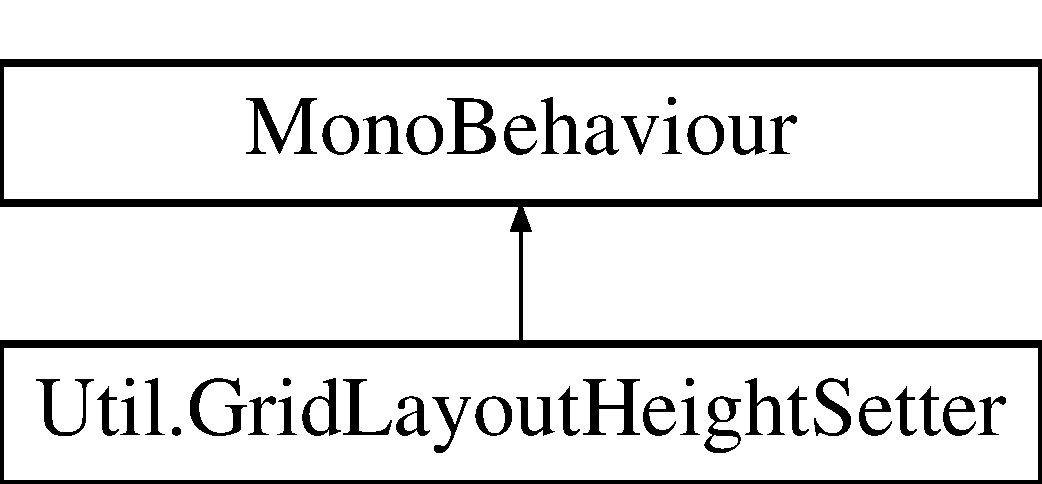
\includegraphics[height=2.000000cm]{class_util_1_1_grid_layout_height_setter}
\end{center}
\end{figure}
\subsection*{Public Attributes}
\begin{DoxyCompactItemize}
\item 
bool {\bfseries only\+Use\+Active}\hypertarget{class_util_1_1_grid_layout_height_setter_aee87be52cfc38b73cf5bbc7d2a1cf1a6}{}\label{class_util_1_1_grid_layout_height_setter_aee87be52cfc38b73cf5bbc7d2a1cf1a6}

\end{DoxyCompactItemize}


The documentation for this class was generated from the following file\+:\begin{DoxyCompactItemize}
\item 
Assets/\+Scripts/\+Util/Grid\+Layout\+Height\+Setter.\+cs\end{DoxyCompactItemize}

\hypertarget{class_util_1_1_gridlayout_width_setter}{}\section{Util.\+Gridlayout\+Width\+Setter Class Reference}
\label{class_util_1_1_gridlayout_width_setter}\index{Util.\+Gridlayout\+Width\+Setter@{Util.\+Gridlayout\+Width\+Setter}}
Inheritance diagram for Util.\+Gridlayout\+Width\+Setter\+:\begin{figure}[H]
\begin{center}
\leavevmode
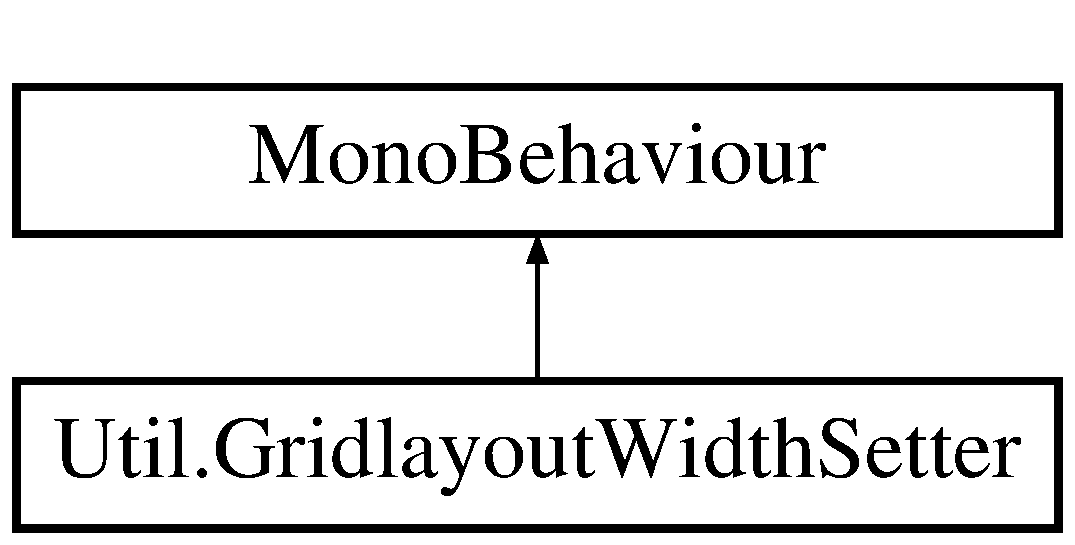
\includegraphics[height=2.000000cm]{class_util_1_1_gridlayout_width_setter}
\end{center}
\end{figure}
\subsection*{Public Member Functions}
\begin{DoxyCompactItemize}
\item 
void {\bfseries Force\+Update} ()\hypertarget{class_util_1_1_gridlayout_width_setter_ad9ab685b813af9f1bcfbc3fa7b503ab3}{}\label{class_util_1_1_gridlayout_width_setter_ad9ab685b813af9f1bcfbc3fa7b503ab3}

\end{DoxyCompactItemize}
\subsection*{Public Attributes}
\begin{DoxyCompactItemize}
\item 
int {\bfseries Children\+Needed\+To\+Scroll} = 8\hypertarget{class_util_1_1_gridlayout_width_setter_a5c62a3430984c0475f0eaa7f8d674136}{}\label{class_util_1_1_gridlayout_width_setter_a5c62a3430984c0475f0eaa7f8d674136}

\item 
bool {\bfseries only\+Set\+Container\+Height} = true\hypertarget{class_util_1_1_gridlayout_width_setter_ab4051adeb77773dbb4c897d4b1edfb04}{}\label{class_util_1_1_gridlayout_width_setter_ab4051adeb77773dbb4c897d4b1edfb04}

\item 
bool {\bfseries only\+Use\+Active\+Children} = true\hypertarget{class_util_1_1_gridlayout_width_setter_ab0b3f268db6cd516808f306dde347f07}{}\label{class_util_1_1_gridlayout_width_setter_ab0b3f268db6cd516808f306dde347f07}

\end{DoxyCompactItemize}


The documentation for this class was generated from the following file\+:\begin{DoxyCompactItemize}
\item 
Assets/\+Scripts/\+Util/Gridlayout\+Width\+Setter.\+cs\end{DoxyCompactItemize}

\hypertarget{class_menus_1_1_high_score_display_object}{}\section{Menus.\+High\+Score\+Display\+Object Class Reference}
\label{class_menus_1_1_high_score_display_object}\index{Menus.\+High\+Score\+Display\+Object@{Menus.\+High\+Score\+Display\+Object}}


A display object for in the highscore screen  


Inheritance diagram for Menus.\+High\+Score\+Display\+Object\+:\begin{figure}[H]
\begin{center}
\leavevmode
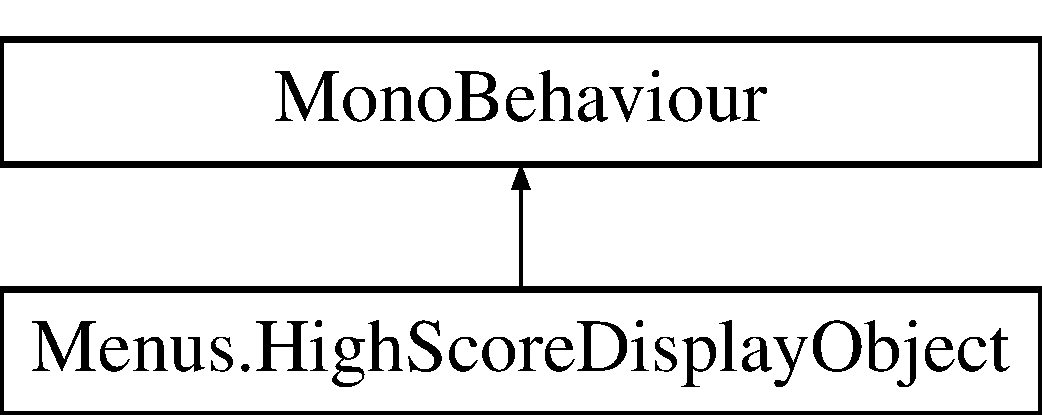
\includegraphics[height=2.000000cm]{class_menus_1_1_high_score_display_object}
\end{center}
\end{figure}
\subsection*{Public Member Functions}
\begin{DoxyCompactItemize}
\item 
void \hyperlink{class_menus_1_1_high_score_display_object_a4826d2032c3e4745c7f775335574fabd}{Set\+Values} (string Name, string Score, Color background\+Color)
\begin{DoxyCompactList}\small\item\em Sets the value that will be displayed \end{DoxyCompactList}\end{DoxyCompactItemize}
\subsection*{Properties}
\begin{DoxyCompactItemize}
\item 
Unity\+Engine.\+U\+I.\+Text {\bfseries Name}\hspace{0.3cm}{\ttfamily  \mbox{[}get\mbox{]}}\hypertarget{class_menus_1_1_high_score_display_object_a6f5e66f0fb2cedc20f3665d91eb32a14}{}\label{class_menus_1_1_high_score_display_object_a6f5e66f0fb2cedc20f3665d91eb32a14}

\item 
Unity\+Engine.\+U\+I.\+Text {\bfseries Score}\hspace{0.3cm}{\ttfamily  \mbox{[}get\mbox{]}}\hypertarget{class_menus_1_1_high_score_display_object_ac75150470bff753ad209980ca41744d3}{}\label{class_menus_1_1_high_score_display_object_ac75150470bff753ad209980ca41744d3}

\end{DoxyCompactItemize}


\subsection{Detailed Description}
A display object for in the highscore screen 



\subsection{Member Function Documentation}
\index{Menus\+::\+High\+Score\+Display\+Object@{Menus\+::\+High\+Score\+Display\+Object}!Set\+Values@{Set\+Values}}
\index{Set\+Values@{Set\+Values}!Menus\+::\+High\+Score\+Display\+Object@{Menus\+::\+High\+Score\+Display\+Object}}
\subsubsection[{\texorpdfstring{Set\+Values(string Name, string Score, Color background\+Color)}{SetValues(string Name, string Score, Color backgroundColor)}}]{\setlength{\rightskip}{0pt plus 5cm}void Menus.\+High\+Score\+Display\+Object.\+Set\+Values (
\begin{DoxyParamCaption}
\item[{string}]{Name, }
\item[{string}]{Score, }
\item[{Color}]{background\+Color}
\end{DoxyParamCaption}
)\hspace{0.3cm}{\ttfamily [inline]}}\hypertarget{class_menus_1_1_high_score_display_object_a4826d2032c3e4745c7f775335574fabd}{}\label{class_menus_1_1_high_score_display_object_a4826d2032c3e4745c7f775335574fabd}


Sets the value that will be displayed 


\begin{DoxyParams}{Parameters}
{\em Name} & Name of the player that submited the score\\
\hline
{\em Score} & Score the player got\\
\hline
{\em background\+Color} & The color the background will be having\\
\hline
\end{DoxyParams}


The documentation for this class was generated from the following file\+:\begin{DoxyCompactItemize}
\item 
Assets/\+Scripts/\+U\+I/\+High\+Score/High\+Score\+Display\+Object.\+cs\end{DoxyCompactItemize}

\hypertarget{class_menus_1_1_high_score_menu}{}\section{Menus.\+High\+Score\+Menu Class Reference}
\label{class_menus_1_1_high_score_menu}\index{Menus.\+High\+Score\+Menu@{Menus.\+High\+Score\+Menu}}
Inheritance diagram for Menus.\+High\+Score\+Menu\+:\begin{figure}[H]
\begin{center}
\leavevmode
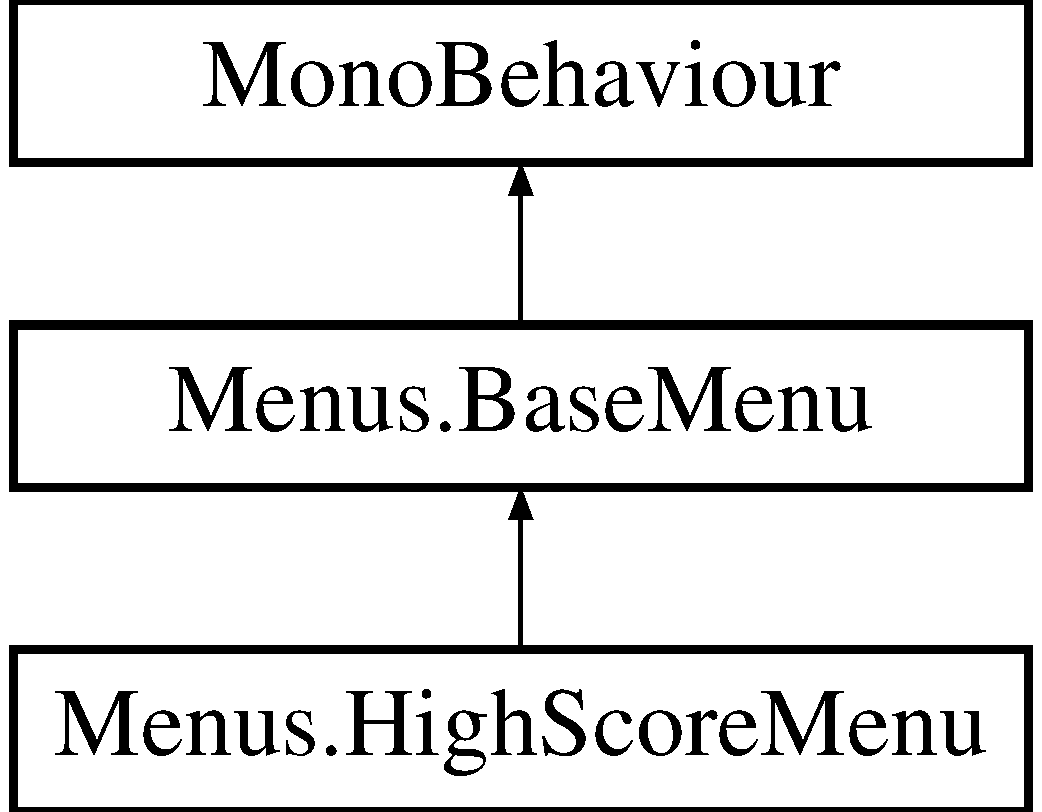
\includegraphics[height=3.000000cm]{class_menus_1_1_high_score_menu}
\end{center}
\end{figure}
\subsection*{Additional Inherited Members}


The documentation for this class was generated from the following file\+:\begin{DoxyCompactItemize}
\item 
Assets/\+Scripts/\+U\+I/\+High\+Score/High\+Score\+Menu.\+cs\end{DoxyCompactItemize}

\hypertarget{class_menus_1_1_high_score_submit_screen}{}\section{Menus.\+High\+Score\+Submit\+Screen Class Reference}
\label{class_menus_1_1_high_score_submit_screen}\index{Menus.\+High\+Score\+Submit\+Screen@{Menus.\+High\+Score\+Submit\+Screen}}
Inheritance diagram for Menus.\+High\+Score\+Submit\+Screen\+:\begin{figure}[H]
\begin{center}
\leavevmode
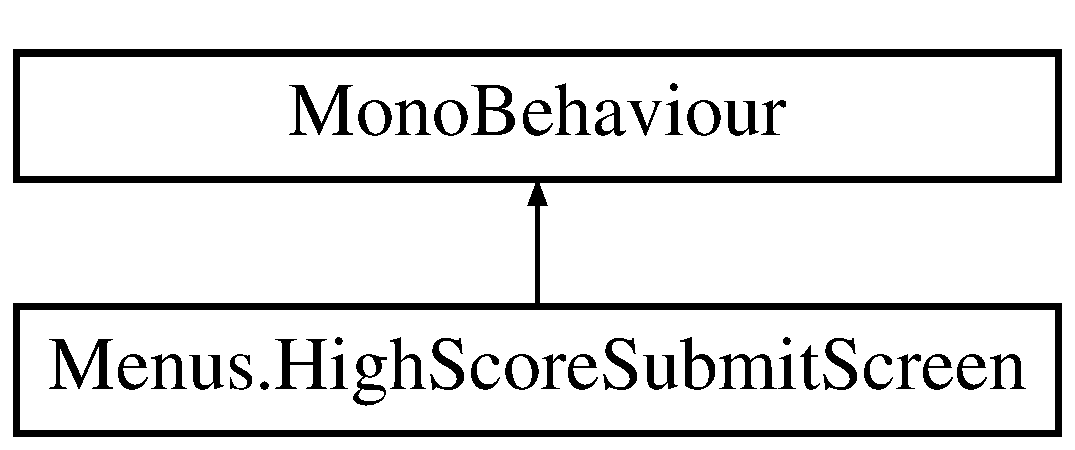
\includegraphics[height=2.000000cm]{class_menus_1_1_high_score_submit_screen}
\end{center}
\end{figure}
\subsection*{Public Member Functions}
\begin{DoxyCompactItemize}
\item 
void {\bfseries Open} ()\hypertarget{class_menus_1_1_high_score_submit_screen_adab4198bdc0053b59cb6a3da0a0c70e7}{}\label{class_menus_1_1_high_score_submit_screen_adab4198bdc0053b59cb6a3da0a0c70e7}

\item 
void {\bfseries Submit} ()\hypertarget{class_menus_1_1_high_score_submit_screen_a996f795250986263f1dc173cc2b5e288}{}\label{class_menus_1_1_high_score_submit_screen_a996f795250986263f1dc173cc2b5e288}

\item 
void {\bfseries Cancel} ()\hypertarget{class_menus_1_1_high_score_submit_screen_ab60152aa7d1bf96cc792f96d62a4cb03}{}\label{class_menus_1_1_high_score_submit_screen_ab60152aa7d1bf96cc792f96d62a4cb03}

\item 
void {\bfseries Close} ()\hypertarget{class_menus_1_1_high_score_submit_screen_a0ebeed644044395b4b86fcc90252cf4a}{}\label{class_menus_1_1_high_score_submit_screen_a0ebeed644044395b4b86fcc90252cf4a}

\end{DoxyCompactItemize}
\subsection*{Events}
\begin{DoxyCompactItemize}
\item 
Void\+Delegate {\bfseries on\+Close}\hypertarget{class_menus_1_1_high_score_submit_screen_abc17caf0db722b74ea43529a597234a2}{}\label{class_menus_1_1_high_score_submit_screen_abc17caf0db722b74ea43529a597234a2}

\end{DoxyCompactItemize}


The documentation for this class was generated from the following file\+:\begin{DoxyCompactItemize}
\item 
Assets/\+Scripts/\+U\+I/\+High\+Score/High\+Score\+Submit\+Screen.\+cs\end{DoxyCompactItemize}

\hypertarget{class_events_1_1_i_ball_hit_bottom}{}\section{Events.\+I\+Ball\+Hit\+Bottom Class Reference}
\label{class_events_1_1_i_ball_hit_bottom}\index{Events.\+I\+Ball\+Hit\+Bottom@{Events.\+I\+Ball\+Hit\+Bottom}}


Empty event class that is called when the player hits the ground  


Inheritance diagram for Events.\+I\+Ball\+Hit\+Bottom\+:\begin{figure}[H]
\begin{center}
\leavevmode
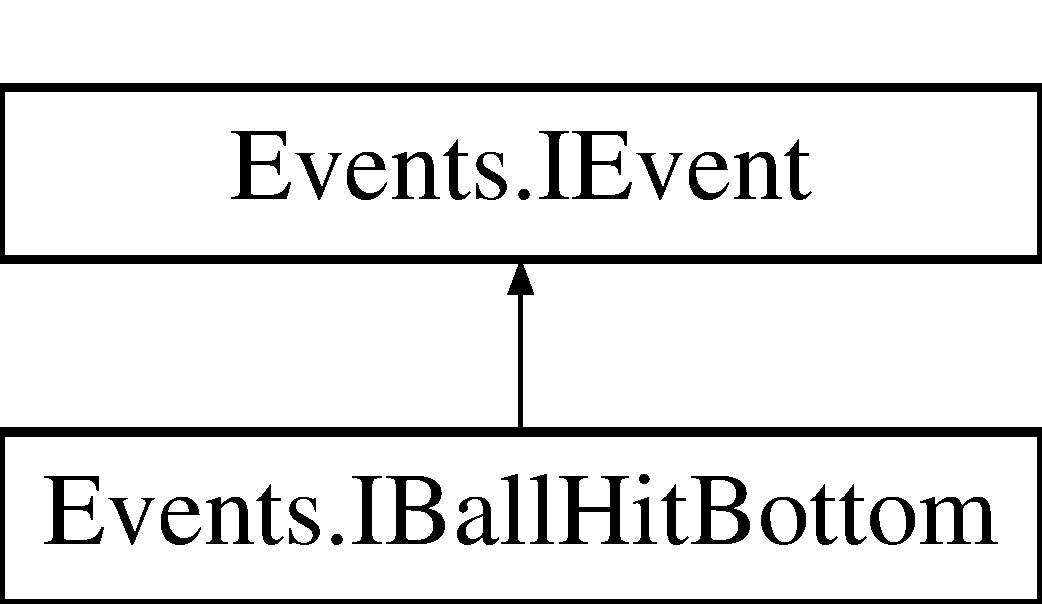
\includegraphics[height=2.000000cm]{class_events_1_1_i_ball_hit_bottom}
\end{center}
\end{figure}


\subsection{Detailed Description}
Empty event class that is called when the player hits the ground 



The documentation for this class was generated from the following file\+:\begin{DoxyCompactItemize}
\item 
Assets/\+Scripts/\+Events/I\+Player\+Hit\+Bottom.\+cs\end{DoxyCompactItemize}

\hypertarget{class_events_1_1_i_ball_move}{}\section{Events.\+I\+Ball\+Move Class Reference}
\label{class_events_1_1_i_ball_move}\index{Events.\+I\+Ball\+Move@{Events.\+I\+Ball\+Move}}


Called when the ball moves  


Inheritance diagram for Events.\+I\+Ball\+Move\+:\begin{figure}[H]
\begin{center}
\leavevmode
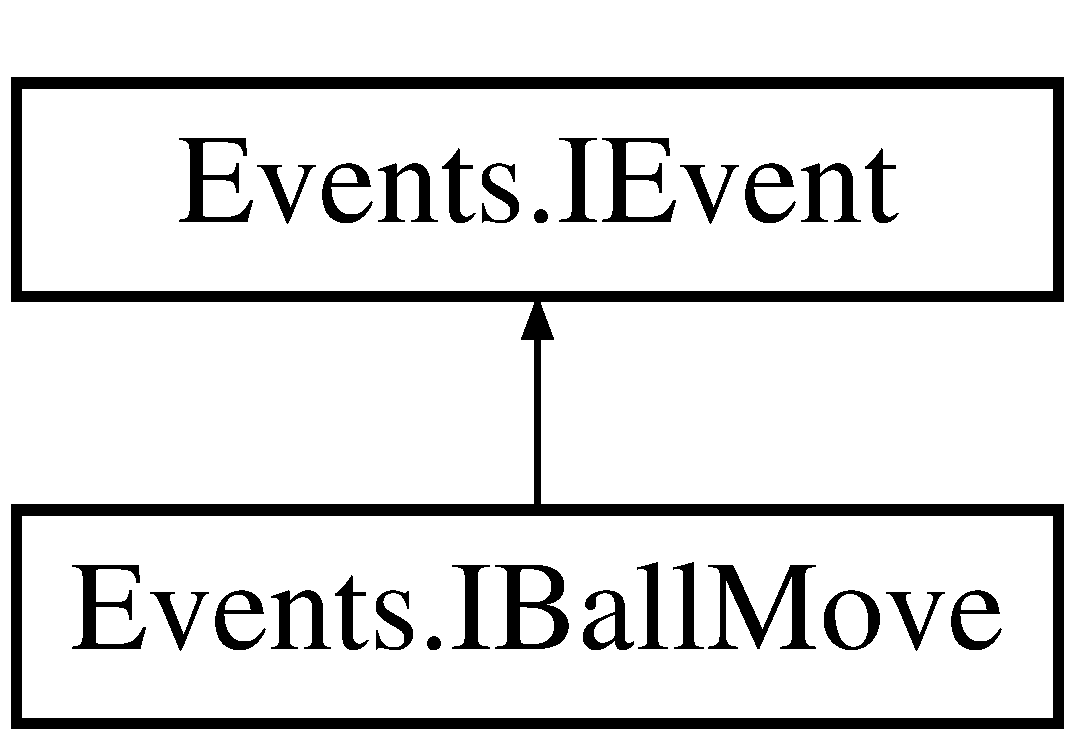
\includegraphics[height=2.000000cm]{class_events_1_1_i_ball_move}
\end{center}
\end{figure}
\subsection*{Public Member Functions}
\begin{DoxyCompactItemize}
\item 
{\bfseries I\+Ball\+Move} (Vector2 \hyperlink{class_events_1_1_i_ball_move_aaa7ee0633897f9e4e56467a46d56e3cc}{direction}, Vector2 \hyperlink{class_events_1_1_i_ball_move_a15ca83aec7e67497dd36c046fca0bbd7}{position})\hypertarget{class_events_1_1_i_ball_move_aff7115d9719a72e1fbb7718a10a93860}{}\label{class_events_1_1_i_ball_move_aff7115d9719a72e1fbb7718a10a93860}

\end{DoxyCompactItemize}
\subsection*{Public Attributes}
\begin{DoxyCompactItemize}
\item 
Vector2 \hyperlink{class_events_1_1_i_ball_move_aaa7ee0633897f9e4e56467a46d56e3cc}{direction} = Vector2.\+zero
\begin{DoxyCompactList}\small\item\em Current direction the ball moves in Values are between -\/1 and 1 \end{DoxyCompactList}\item 
Vector2 \hyperlink{class_events_1_1_i_ball_move_a15ca83aec7e67497dd36c046fca0bbd7}{position} = Vector2.\+zero
\begin{DoxyCompactList}\small\item\em The position of the ball at the moment of clicking \end{DoxyCompactList}\end{DoxyCompactItemize}


\subsection{Detailed Description}
Called when the ball moves 



\subsection{Member Data Documentation}
\index{Events\+::\+I\+Ball\+Move@{Events\+::\+I\+Ball\+Move}!direction@{direction}}
\index{direction@{direction}!Events\+::\+I\+Ball\+Move@{Events\+::\+I\+Ball\+Move}}
\subsubsection[{\texorpdfstring{direction}{direction}}]{\setlength{\rightskip}{0pt plus 5cm}Vector2 Events.\+I\+Ball\+Move.\+direction = Vector2.\+zero}\hypertarget{class_events_1_1_i_ball_move_aaa7ee0633897f9e4e56467a46d56e3cc}{}\label{class_events_1_1_i_ball_move_aaa7ee0633897f9e4e56467a46d56e3cc}


Current direction the ball moves in Values are between -\/1 and 1 

\index{Events\+::\+I\+Ball\+Move@{Events\+::\+I\+Ball\+Move}!position@{position}}
\index{position@{position}!Events\+::\+I\+Ball\+Move@{Events\+::\+I\+Ball\+Move}}
\subsubsection[{\texorpdfstring{position}{position}}]{\setlength{\rightskip}{0pt plus 5cm}Vector2 Events.\+I\+Ball\+Move.\+position = Vector2.\+zero}\hypertarget{class_events_1_1_i_ball_move_a15ca83aec7e67497dd36c046fca0bbd7}{}\label{class_events_1_1_i_ball_move_a15ca83aec7e67497dd36c046fca0bbd7}


The position of the ball at the moment of clicking 



The documentation for this class was generated from the following file\+:\begin{DoxyCompactItemize}
\item 
Assets/\+Scripts/\+Events/I\+Ball\+Move.\+cs\end{DoxyCompactItemize}

\hypertarget{interface_events_1_1_i_event}{}\section{Events.\+I\+Event Interface Reference}
\label{interface_events_1_1_i_event}\index{Events.\+I\+Event@{Events.\+I\+Event}}


The base interface for \hyperlink{namespace_events}{Events}.  


Inheritance diagram for Events.\+I\+Event\+:\begin{figure}[H]
\begin{center}
\leavevmode
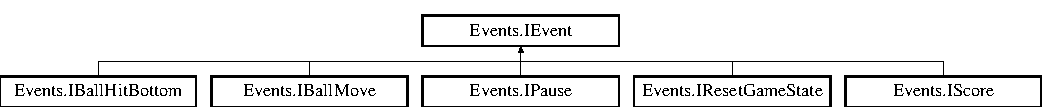
\includegraphics[height=1.794872cm]{interface_events_1_1_i_event}
\end{center}
\end{figure}


\subsection{Detailed Description}
The base interface for \hyperlink{namespace_events}{Events}. 



The documentation for this interface was generated from the following file\+:\begin{DoxyCompactItemize}
\item 
Assets/\+Scripts/\+Util/\+Events/I\+Event.\+cs\end{DoxyCompactItemize}

\hypertarget{interface_events_1_1_i_event_dispatcher}{}\section{Events.\+I\+Event\+Dispatcher Interface Reference}
\label{interface_events_1_1_i_event_dispatcher}\index{Events.\+I\+Event\+Dispatcher@{Events.\+I\+Event\+Dispatcher}}


Event dispatcher interface.  


Inheritance diagram for Events.\+I\+Event\+Dispatcher\+:\begin{figure}[H]
\begin{center}
\leavevmode
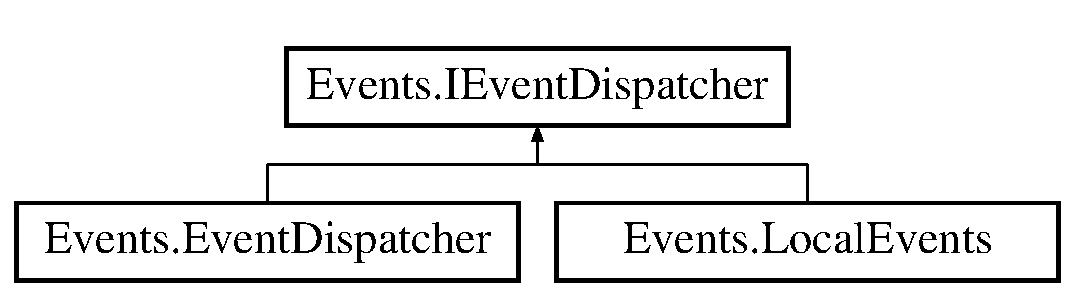
\includegraphics[height=2.000000cm]{interface_events_1_1_i_event_dispatcher}
\end{center}
\end{figure}
\subsection*{Public Member Functions}
\begin{DoxyCompactItemize}
\item 
void \hyperlink{interface_events_1_1_i_event_dispatcher_ac22d58973ca79fdaea1471704dba0e01}{Add\+Event\+Listener} (Type type, Action handler)
\begin{DoxyCompactList}\small\item\em Add an event listener. \end{DoxyCompactList}\item 
void \hyperlink{interface_events_1_1_i_event_dispatcher_a4c10e52a26a0c354bcaae21e0a240f93}{Add\+Event\+Listener$<$ T $>$} (Action$<$ T $>$ handler)
\begin{DoxyCompactList}\small\item\em Add an event listener. \end{DoxyCompactList}\item 
void \hyperlink{interface_events_1_1_i_event_dispatcher_ae3209681ebdbcf8289905ff6ccdbd188}{Remove\+Event\+Listener} (Type type, Action handler)
\begin{DoxyCompactList}\small\item\em Remove an event listener. \end{DoxyCompactList}\item 
void \hyperlink{interface_events_1_1_i_event_dispatcher_a86e3438c779746108c3f01dff0c43d23}{Remove\+Event\+Listener$<$ T $>$} (Action$<$ T $>$ handler)
\begin{DoxyCompactList}\small\item\em Remove an event listener. \end{DoxyCompactList}\item 
void \hyperlink{interface_events_1_1_i_event_dispatcher_a3789c396884e0097a4efdd8fb6652214}{Invoke} (Type type, object evt)
\begin{DoxyCompactList}\small\item\em Invoke an event. \end{DoxyCompactList}\item 
void \hyperlink{interface_events_1_1_i_event_dispatcher_ab6e50172a6c4a5ec91977f183278dc91}{Invoke$<$ T $>$} (T evt)
\begin{DoxyCompactList}\small\item\em Invoke an event. \end{DoxyCompactList}\end{DoxyCompactItemize}


\subsection{Detailed Description}
Event dispatcher interface. 



\subsection{Member Function Documentation}
\index{Events\+::\+I\+Event\+Dispatcher@{Events\+::\+I\+Event\+Dispatcher}!Add\+Event\+Listener@{Add\+Event\+Listener}}
\index{Add\+Event\+Listener@{Add\+Event\+Listener}!Events\+::\+I\+Event\+Dispatcher@{Events\+::\+I\+Event\+Dispatcher}}
\subsubsection[{\texorpdfstring{Add\+Event\+Listener(\+Type type, Action handler)}{AddEventListener(Type type, Action handler)}}]{\setlength{\rightskip}{0pt plus 5cm}void Events.\+I\+Event\+Dispatcher.\+Add\+Event\+Listener (
\begin{DoxyParamCaption}
\item[{Type}]{type, }
\item[{Action}]{handler}
\end{DoxyParamCaption}
)}\hypertarget{interface_events_1_1_i_event_dispatcher_ac22d58973ca79fdaea1471704dba0e01}{}\label{interface_events_1_1_i_event_dispatcher_ac22d58973ca79fdaea1471704dba0e01}


Add an event listener. 


\begin{DoxyParams}{Parameters}
{\em type} & The type of the event.\\
\hline
{\em handler} & The handler for the event.\\
\hline
\end{DoxyParams}


Implemented in \hyperlink{class_events_1_1_local_events_aab44ef55c79a59a0b1679207daf32a49}{Events.\+Local\+Events}, and \hyperlink{class_events_1_1_event_dispatcher_af8047b3f53861d56c27aa02e358486a2}{Events.\+Event\+Dispatcher}.

\index{Events\+::\+I\+Event\+Dispatcher@{Events\+::\+I\+Event\+Dispatcher}!Add\+Event\+Listener$<$ T $>$@{Add\+Event\+Listener$<$ T $>$}}
\index{Add\+Event\+Listener$<$ T $>$@{Add\+Event\+Listener$<$ T $>$}!Events\+::\+I\+Event\+Dispatcher@{Events\+::\+I\+Event\+Dispatcher}}
\subsubsection[{\texorpdfstring{Add\+Event\+Listener$<$ T $>$(\+Action$<$ T $>$ handler)}{AddEventListener< T >(Action< T > handler)}}]{\setlength{\rightskip}{0pt plus 5cm}void {\bf Events.\+I\+Event\+Dispatcher.\+Add\+Event\+Listener}$<$ T $>$ (
\begin{DoxyParamCaption}
\item[{Action$<$ T $>$}]{handler}
\end{DoxyParamCaption}
)}\hypertarget{interface_events_1_1_i_event_dispatcher_a4c10e52a26a0c354bcaae21e0a240f93}{}\label{interface_events_1_1_i_event_dispatcher_a4c10e52a26a0c354bcaae21e0a240f93}


Add an event listener. 


\begin{DoxyTemplParams}{Template Parameters}
{\em T} & The type of the event.\\
\hline
\end{DoxyTemplParams}

\begin{DoxyParams}{Parameters}
{\em handler} & The handler for the event.\\
\hline
\end{DoxyParams}


Implemented in \hyperlink{class_events_1_1_event_dispatcher_ab90178e5a5bbfd90601347ab8489cf01}{Events.\+Event\+Dispatcher}, and \hyperlink{class_events_1_1_local_events_add06ea2d4511cbf585df741b09d54742}{Events.\+Local\+Events}.

\begin{Desc}
\item[Type Constraints]\begin{description}
\item[{\em T} : {\em I\+Event}]\end{description}
\end{Desc}
\index{Events\+::\+I\+Event\+Dispatcher@{Events\+::\+I\+Event\+Dispatcher}!Invoke@{Invoke}}
\index{Invoke@{Invoke}!Events\+::\+I\+Event\+Dispatcher@{Events\+::\+I\+Event\+Dispatcher}}
\subsubsection[{\texorpdfstring{Invoke(\+Type type, object evt)}{Invoke(Type type, object evt)}}]{\setlength{\rightskip}{0pt plus 5cm}void Events.\+I\+Event\+Dispatcher.\+Invoke (
\begin{DoxyParamCaption}
\item[{Type}]{type, }
\item[{object}]{evt}
\end{DoxyParamCaption}
)}\hypertarget{interface_events_1_1_i_event_dispatcher_a3789c396884e0097a4efdd8fb6652214}{}\label{interface_events_1_1_i_event_dispatcher_a3789c396884e0097a4efdd8fb6652214}


Invoke an event. 


\begin{DoxyParams}{Parameters}
{\em type} & The type of event to be invoked.\\
\hline
{\em evt} & The event to be invoked.\\
\hline
\end{DoxyParams}


Implemented in \hyperlink{class_events_1_1_event_dispatcher_a4bec3274dceea156c52248cac71e968c}{Events.\+Event\+Dispatcher}, and \hyperlink{class_events_1_1_local_events_a4464675f72b8e310902f22770f4be0f4}{Events.\+Local\+Events}.

\index{Events\+::\+I\+Event\+Dispatcher@{Events\+::\+I\+Event\+Dispatcher}!Invoke$<$ T $>$@{Invoke$<$ T $>$}}
\index{Invoke$<$ T $>$@{Invoke$<$ T $>$}!Events\+::\+I\+Event\+Dispatcher@{Events\+::\+I\+Event\+Dispatcher}}
\subsubsection[{\texorpdfstring{Invoke$<$ T $>$(\+T evt)}{Invoke< T >(T evt)}}]{\setlength{\rightskip}{0pt plus 5cm}void {\bf Events.\+I\+Event\+Dispatcher.\+Invoke}$<$ T $>$ (
\begin{DoxyParamCaption}
\item[{T}]{evt}
\end{DoxyParamCaption}
)}\hypertarget{interface_events_1_1_i_event_dispatcher_ab6e50172a6c4a5ec91977f183278dc91}{}\label{interface_events_1_1_i_event_dispatcher_ab6e50172a6c4a5ec91977f183278dc91}


Invoke an event. 


\begin{DoxyTemplParams}{Template Parameters}
{\em T} & The type of event to be invoked.\\
\hline
\end{DoxyTemplParams}

\begin{DoxyParams}{Parameters}
{\em evt} & The event to be invoked.\\
\hline
\end{DoxyParams}


Implemented in \hyperlink{class_events_1_1_event_dispatcher_a7c1fe1b9738ea149420d19c1131f2f25}{Events.\+Event\+Dispatcher}, and \hyperlink{class_events_1_1_local_events_a1e67a61a570a8105c018c366b54959c6}{Events.\+Local\+Events}.

\begin{Desc}
\item[Type Constraints]\begin{description}
\item[{\em T} : {\em I\+Event}]\end{description}
\end{Desc}
\index{Events\+::\+I\+Event\+Dispatcher@{Events\+::\+I\+Event\+Dispatcher}!Remove\+Event\+Listener@{Remove\+Event\+Listener}}
\index{Remove\+Event\+Listener@{Remove\+Event\+Listener}!Events\+::\+I\+Event\+Dispatcher@{Events\+::\+I\+Event\+Dispatcher}}
\subsubsection[{\texorpdfstring{Remove\+Event\+Listener(\+Type type, Action handler)}{RemoveEventListener(Type type, Action handler)}}]{\setlength{\rightskip}{0pt plus 5cm}void Events.\+I\+Event\+Dispatcher.\+Remove\+Event\+Listener (
\begin{DoxyParamCaption}
\item[{Type}]{type, }
\item[{Action}]{handler}
\end{DoxyParamCaption}
)}\hypertarget{interface_events_1_1_i_event_dispatcher_ae3209681ebdbcf8289905ff6ccdbd188}{}\label{interface_events_1_1_i_event_dispatcher_ae3209681ebdbcf8289905ff6ccdbd188}


Remove an event listener. 


\begin{DoxyParams}{Parameters}
{\em type} & The type of the event.\\
\hline
{\em handler} & The handler.\\
\hline
\end{DoxyParams}


Implemented in \hyperlink{class_events_1_1_event_dispatcher_a9644ebc4fb5655cda345b586e5749ea0}{Events.\+Event\+Dispatcher}, and \hyperlink{class_events_1_1_local_events_acff4973a06ab3ce4bd0a2c8adbe54e2b}{Events.\+Local\+Events}.

\index{Events\+::\+I\+Event\+Dispatcher@{Events\+::\+I\+Event\+Dispatcher}!Remove\+Event\+Listener$<$ T $>$@{Remove\+Event\+Listener$<$ T $>$}}
\index{Remove\+Event\+Listener$<$ T $>$@{Remove\+Event\+Listener$<$ T $>$}!Events\+::\+I\+Event\+Dispatcher@{Events\+::\+I\+Event\+Dispatcher}}
\subsubsection[{\texorpdfstring{Remove\+Event\+Listener$<$ T $>$(\+Action$<$ T $>$ handler)}{RemoveEventListener< T >(Action< T > handler)}}]{\setlength{\rightskip}{0pt plus 5cm}void {\bf Events.\+I\+Event\+Dispatcher.\+Remove\+Event\+Listener}$<$ T $>$ (
\begin{DoxyParamCaption}
\item[{Action$<$ T $>$}]{handler}
\end{DoxyParamCaption}
)}\hypertarget{interface_events_1_1_i_event_dispatcher_a86e3438c779746108c3f01dff0c43d23}{}\label{interface_events_1_1_i_event_dispatcher_a86e3438c779746108c3f01dff0c43d23}


Remove an event listener. 


\begin{DoxyTemplParams}{Template Parameters}
{\em T} & The type of the event.\\
\hline
\end{DoxyTemplParams}

\begin{DoxyParams}{Parameters}
{\em handler} & The handler.\\
\hline
\end{DoxyParams}


Implemented in \hyperlink{class_events_1_1_event_dispatcher_a88f24cbfab1022517830b3fc42155c15}{Events.\+Event\+Dispatcher}, and \hyperlink{class_events_1_1_local_events_ac8647cb9efdd5e6b86362908a8019cad}{Events.\+Local\+Events}.

\begin{Desc}
\item[Type Constraints]\begin{description}
\item[{\em T} : {\em I\+Event}]\end{description}
\end{Desc}


The documentation for this interface was generated from the following file\+:\begin{DoxyCompactItemize}
\item 
Assets/\+Scripts/\+Util/\+Events/I\+Event\+Dispatcher.\+cs\end{DoxyCompactItemize}

\hypertarget{class_input_manager}{}\section{Input\+Manager Class Reference}
\label{class_input_manager}\index{Input\+Manager@{Input\+Manager}}
Inheritance diagram for Input\+Manager\+:\begin{figure}[H]
\begin{center}
\leavevmode
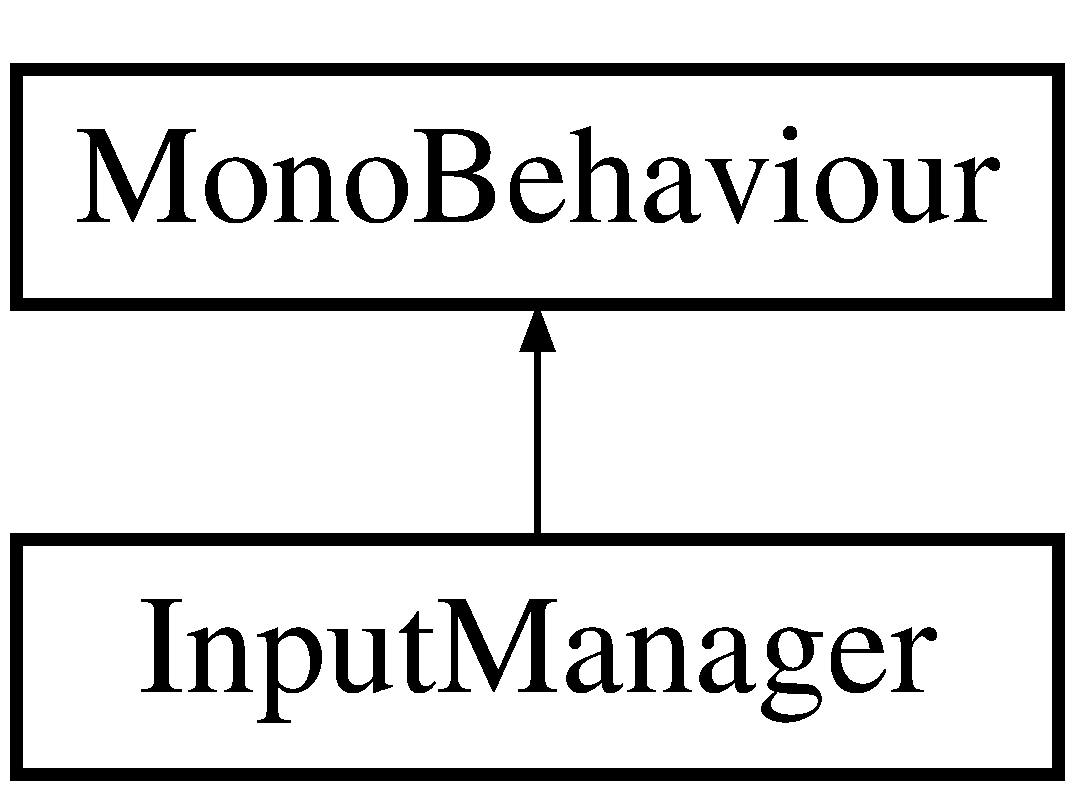
\includegraphics[height=2.000000cm]{class_input_manager}
\end{center}
\end{figure}
\subsection*{Public Member Functions}
\begin{DoxyCompactItemize}
\item 
void {\bfseries On\+Destroy} ()\hypertarget{class_input_manager_ae45098c58b84ad9d805c20cceee492d0}{}\label{class_input_manager_ae45098c58b84ad9d805c20cceee492d0}

\end{DoxyCompactItemize}
\subsection*{Events}
\begin{DoxyCompactItemize}
\item 
static Click\+Delegate \hyperlink{class_input_manager_a1cc95536c19ed45ce645e20aca69755e}{on\+Click}
\begin{DoxyCompactList}\small\item\em Called when a click is registered on the screen \end{DoxyCompactList}\item 
static Void\+Delegate \hyperlink{class_input_manager_a81a585645cea9e8936c148e0b653df36}{on\+Escape\+Press}
\begin{DoxyCompactList}\small\item\em Called when escape is pressed \end{DoxyCompactList}\end{DoxyCompactItemize}


\subsection{Event Documentation}
\index{Input\+Manager@{Input\+Manager}!on\+Click@{on\+Click}}
\index{on\+Click@{on\+Click}!Input\+Manager@{Input\+Manager}}
\subsubsection[{\texorpdfstring{on\+Click}{onClick}}]{\setlength{\rightskip}{0pt plus 5cm}Click\+Delegate Input\+Manager.\+on\+Click\hspace{0.3cm}{\ttfamily [static]}}\hypertarget{class_input_manager_a1cc95536c19ed45ce645e20aca69755e}{}\label{class_input_manager_a1cc95536c19ed45ce645e20aca69755e}


Called when a click is registered on the screen 

\index{Input\+Manager@{Input\+Manager}!on\+Escape\+Press@{on\+Escape\+Press}}
\index{on\+Escape\+Press@{on\+Escape\+Press}!Input\+Manager@{Input\+Manager}}
\subsubsection[{\texorpdfstring{on\+Escape\+Press}{onEscapePress}}]{\setlength{\rightskip}{0pt plus 5cm}Void\+Delegate Input\+Manager.\+on\+Escape\+Press\hspace{0.3cm}{\ttfamily [static]}}\hypertarget{class_input_manager_a81a585645cea9e8936c148e0b653df36}{}\label{class_input_manager_a81a585645cea9e8936c148e0b653df36}


Called when escape is pressed 



The documentation for this class was generated from the following file\+:\begin{DoxyCompactItemize}
\item 
Assets/\+Scripts/\+Managers/Input\+Manager.\+cs\end{DoxyCompactItemize}

\hypertarget{class_events_1_1_i_pause}{}\section{Events.\+I\+Pause Class Reference}
\label{class_events_1_1_i_pause}\index{Events.\+I\+Pause@{Events.\+I\+Pause}}
Inheritance diagram for Events.\+I\+Pause\+:\begin{figure}[H]
\begin{center}
\leavevmode
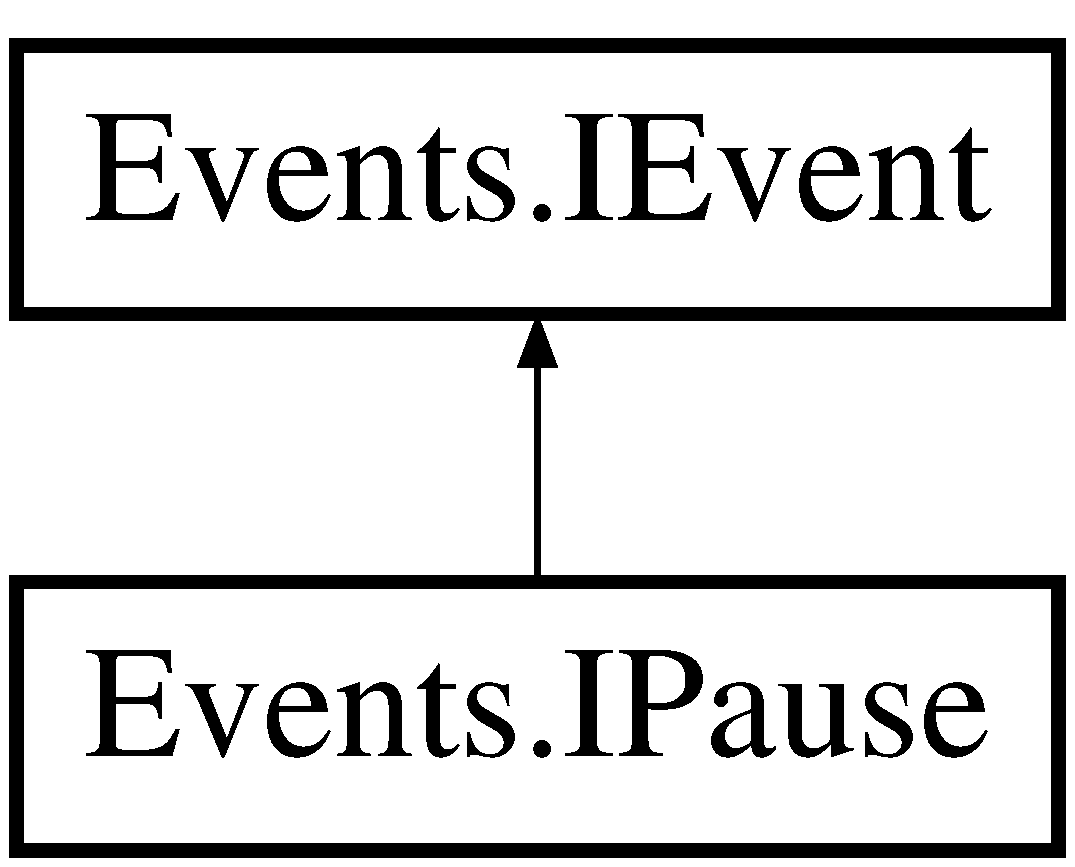
\includegraphics[height=2.000000cm]{class_events_1_1_i_pause}
\end{center}
\end{figure}
\subsection*{Public Member Functions}
\begin{DoxyCompactItemize}
\item 
\hyperlink{class_events_1_1_i_pause_ad5366754b81dc5bc50f8bc14c62ebaa5}{I\+Pause} (bool State)
\begin{DoxyCompactList}\small\item\em Event Class that sends pause state changes to all listeners \end{DoxyCompactList}\end{DoxyCompactItemize}
\subsection*{Public Attributes}
\begin{DoxyCompactItemize}
\item 
bool {\bfseries State}\hypertarget{class_events_1_1_i_pause_afc11e9a193f36974f990775429eee9cc}{}\label{class_events_1_1_i_pause_afc11e9a193f36974f990775429eee9cc}

\end{DoxyCompactItemize}


\subsection{Constructor \& Destructor Documentation}
\index{Events\+::\+I\+Pause@{Events\+::\+I\+Pause}!I\+Pause@{I\+Pause}}
\index{I\+Pause@{I\+Pause}!Events\+::\+I\+Pause@{Events\+::\+I\+Pause}}
\subsubsection[{\texorpdfstring{I\+Pause(bool State)}{IPause(bool State)}}]{\setlength{\rightskip}{0pt plus 5cm}Events.\+I\+Pause.\+I\+Pause (
\begin{DoxyParamCaption}
\item[{bool}]{State}
\end{DoxyParamCaption}
)\hspace{0.3cm}{\ttfamily [inline]}}\hypertarget{class_events_1_1_i_pause_ad5366754b81dc5bc50f8bc14c62ebaa5}{}\label{class_events_1_1_i_pause_ad5366754b81dc5bc50f8bc14c62ebaa5}


Event Class that sends pause state changes to all listeners 


\begin{DoxyParams}{Parameters}
{\em State} & \\
\hline
\end{DoxyParams}


The documentation for this class was generated from the following file\+:\begin{DoxyCompactItemize}
\item 
Assets/\+Scripts/\+Events/I\+Pause.\+cs\end{DoxyCompactItemize}

\hypertarget{class_events_1_1_i_reset_game_state}{}\section{Events.\+I\+Reset\+Game\+State Class Reference}
\label{class_events_1_1_i_reset_game_state}\index{Events.\+I\+Reset\+Game\+State@{Events.\+I\+Reset\+Game\+State}}


Called when the game requires a restart like when the player goes game over  


Inheritance diagram for Events.\+I\+Reset\+Game\+State\+:\begin{figure}[H]
\begin{center}
\leavevmode
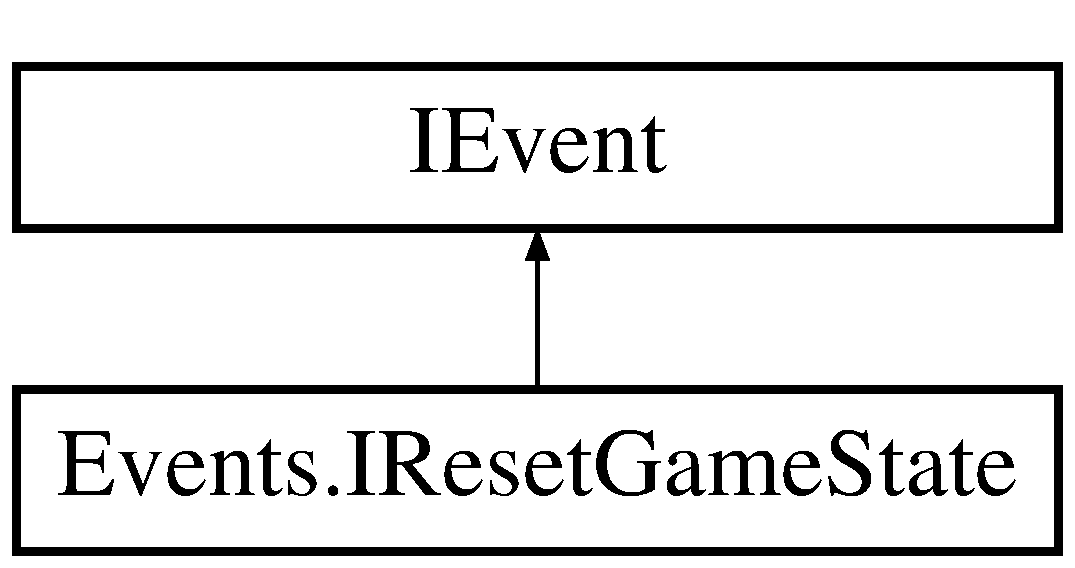
\includegraphics[height=2.000000cm]{class_events_1_1_i_reset_game_state}
\end{center}
\end{figure}


\subsection{Detailed Description}
Called when the game requires a restart like when the player goes game over 



The documentation for this class was generated from the following file\+:\begin{DoxyCompactItemize}
\item 
Assets/\+Scripts/\+Events/I\+Reset\+Game\+State.\+cs\end{DoxyCompactItemize}

\hypertarget{class_events_1_1_i_score}{}\section{Events.\+I\+Score Class Reference}
\label{class_events_1_1_i_score}\index{Events.\+I\+Score@{Events.\+I\+Score}}


Called when the player hits the target  


Inheritance diagram for Events.\+I\+Score\+:\begin{figure}[H]
\begin{center}
\leavevmode
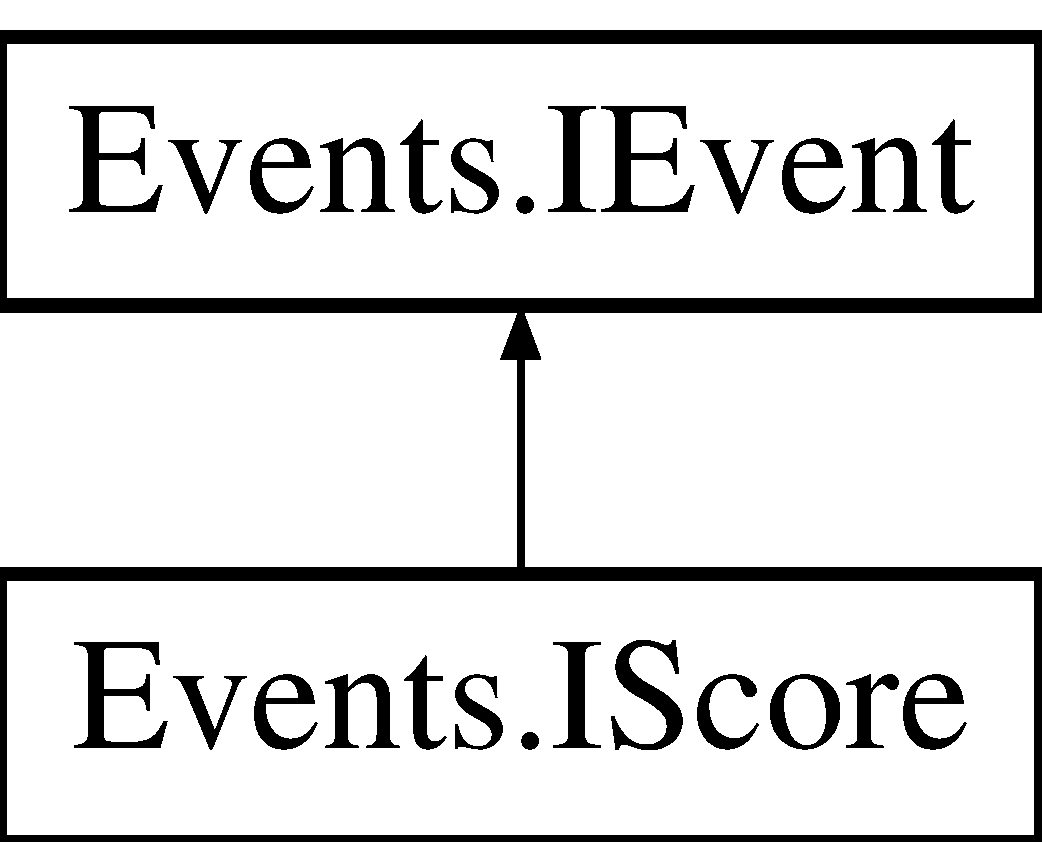
\includegraphics[height=2.000000cm]{class_events_1_1_i_score}
\end{center}
\end{figure}
\subsection*{Public Member Functions}
\begin{DoxyCompactItemize}
\item 
{\bfseries I\+Score} (int \hyperlink{class_events_1_1_i_score_a15ecb3ea31e60c28e8be9bbe8f183409}{bounces}, Vector2 \hyperlink{class_events_1_1_i_score_a2ea657fdd7f72f26c59e92ee71d275d9}{last\+Dir})\hypertarget{class_events_1_1_i_score_ad8997c6b85ecee3394bae7f95cec9113}{}\label{class_events_1_1_i_score_ad8997c6b85ecee3394bae7f95cec9113}

\end{DoxyCompactItemize}
\subsection*{Public Attributes}
\begin{DoxyCompactItemize}
\item 
int \hyperlink{class_events_1_1_i_score_a15ecb3ea31e60c28e8be9bbe8f183409}{bounces} = 0
\begin{DoxyCompactList}\small\item\em Number of times the player bouched against the wall bonus points are given when you hit the walls when you score \end{DoxyCompactList}\item 
Vector2 \hyperlink{class_events_1_1_i_score_a2ea657fdd7f72f26c59e92ee71d275d9}{last\+Dir} = Vector2.\+zero
\begin{DoxyCompactList}\small\item\em The direction the player last clicked. this is so the player can get a bonus if they did a dunk \end{DoxyCompactList}\end{DoxyCompactItemize}


\subsection{Detailed Description}
Called when the player hits the target 



\subsection{Member Data Documentation}
\index{Events\+::\+I\+Score@{Events\+::\+I\+Score}!bounces@{bounces}}
\index{bounces@{bounces}!Events\+::\+I\+Score@{Events\+::\+I\+Score}}
\subsubsection[{\texorpdfstring{bounces}{bounces}}]{\setlength{\rightskip}{0pt plus 5cm}int Events.\+I\+Score.\+bounces = 0}\hypertarget{class_events_1_1_i_score_a15ecb3ea31e60c28e8be9bbe8f183409}{}\label{class_events_1_1_i_score_a15ecb3ea31e60c28e8be9bbe8f183409}


Number of times the player bouched against the wall bonus points are given when you hit the walls when you score 

\index{Events\+::\+I\+Score@{Events\+::\+I\+Score}!last\+Dir@{last\+Dir}}
\index{last\+Dir@{last\+Dir}!Events\+::\+I\+Score@{Events\+::\+I\+Score}}
\subsubsection[{\texorpdfstring{last\+Dir}{lastDir}}]{\setlength{\rightskip}{0pt plus 5cm}Vector2 Events.\+I\+Score.\+last\+Dir = Vector2.\+zero}\hypertarget{class_events_1_1_i_score_a2ea657fdd7f72f26c59e92ee71d275d9}{}\label{class_events_1_1_i_score_a2ea657fdd7f72f26c59e92ee71d275d9}


The direction the player last clicked. this is so the player can get a bonus if they did a dunk 



The documentation for this class was generated from the following file\+:\begin{DoxyCompactItemize}
\item 
Assets/\+Scripts/\+Events/I\+Score.\+cs\end{DoxyCompactItemize}

\hypertarget{class_events_1_1_local_events}{}\section{Events.\+Local\+Events Class Reference}
\label{class_events_1_1_local_events}\index{Events.\+Local\+Events@{Events.\+Local\+Events}}


Use this for local event handling.  


Inheritance diagram for Events.\+Local\+Events\+:\begin{figure}[H]
\begin{center}
\leavevmode
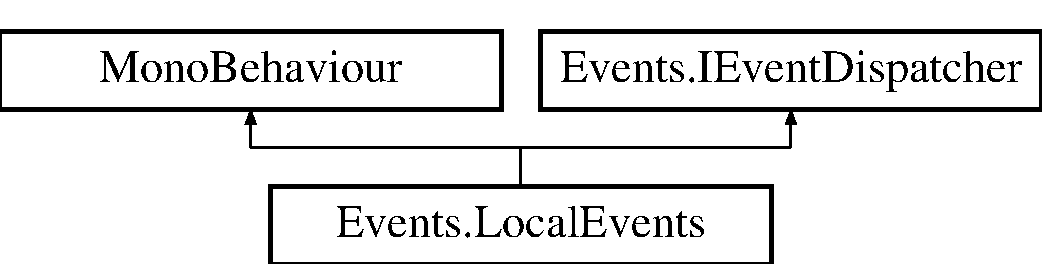
\includegraphics[height=2.000000cm]{class_events_1_1_local_events}
\end{center}
\end{figure}
\subsection*{Public Member Functions}
\begin{DoxyCompactItemize}
\item 
void \hyperlink{class_events_1_1_local_events_aab44ef55c79a59a0b1679207daf32a49}{Add\+Event\+Listener} (Type type, Action handler)
\begin{DoxyCompactList}\small\item\em Implementation of \hyperlink{interface_events_1_1_i_event_dispatcher_ac22d58973ca79fdaea1471704dba0e01}{I\+Event\+Dispatcher.\+Add\+Event\+Listener(\+Type, Action)}. \end{DoxyCompactList}\item 
void \hyperlink{class_events_1_1_local_events_add06ea2d4511cbf585df741b09d54742}{Add\+Event\+Listener$<$ T $>$} (Action$<$ T $>$ handler)
\begin{DoxyCompactList}\small\item\em Implementation of \hyperlink{interface_events_1_1_i_event_dispatcher_a4c10e52a26a0c354bcaae21e0a240f93}{I\+Event\+Dispatcher.\+Add\+Event\+Listener$<$\+T$>$(\+Action$<$\+T$>$)}. \end{DoxyCompactList}\item 
void \hyperlink{class_events_1_1_local_events_acff4973a06ab3ce4bd0a2c8adbe54e2b}{Remove\+Event\+Listener} (Type type, Action handler)
\begin{DoxyCompactList}\small\item\em Implementation of \hyperlink{interface_events_1_1_i_event_dispatcher_ae3209681ebdbcf8289905ff6ccdbd188}{I\+Event\+Dispatcher.\+Remove\+Event\+Listener(\+Type, Action)}. \end{DoxyCompactList}\item 
void \hyperlink{class_events_1_1_local_events_ac8647cb9efdd5e6b86362908a8019cad}{Remove\+Event\+Listener$<$ T $>$} (Action$<$ T $>$ handler)
\begin{DoxyCompactList}\small\item\em Implementation of \hyperlink{interface_events_1_1_i_event_dispatcher_a86e3438c779746108c3f01dff0c43d23}{I\+Event\+Dispatcher.\+Remove\+Event\+Listener$<$\+T$>$(\+Action$<$\+T$>$)}. \end{DoxyCompactList}\item 
void \hyperlink{class_events_1_1_local_events_a4464675f72b8e310902f22770f4be0f4}{Invoke} (Type type, object evt)
\begin{DoxyCompactList}\small\item\em Implementation of I\+Event\+Dispatcher.\+Invoke(\+Type, Action). \end{DoxyCompactList}\item 
void \hyperlink{class_events_1_1_local_events_a1e67a61a570a8105c018c366b54959c6}{Invoke$<$ T $>$} (T evt)
\begin{DoxyCompactList}\small\item\em Implementation of I\+Event\+Dispatcher.\+Invoke$<$\+T$>$(\+Action$<$\+T$>$). \end{DoxyCompactList}\end{DoxyCompactItemize}


\subsection{Detailed Description}
Use this for local event handling. 



\subsection{Member Function Documentation}
\index{Events\+::\+Local\+Events@{Events\+::\+Local\+Events}!Add\+Event\+Listener@{Add\+Event\+Listener}}
\index{Add\+Event\+Listener@{Add\+Event\+Listener}!Events\+::\+Local\+Events@{Events\+::\+Local\+Events}}
\subsubsection[{\texorpdfstring{Add\+Event\+Listener(\+Type type, Action handler)}{AddEventListener(Type type, Action handler)}}]{\setlength{\rightskip}{0pt plus 5cm}void Events.\+Local\+Events.\+Add\+Event\+Listener (
\begin{DoxyParamCaption}
\item[{Type}]{type, }
\item[{Action}]{handler}
\end{DoxyParamCaption}
)\hspace{0.3cm}{\ttfamily [inline]}}\hypertarget{class_events_1_1_local_events_aab44ef55c79a59a0b1679207daf32a49}{}\label{class_events_1_1_local_events_aab44ef55c79a59a0b1679207daf32a49}


Implementation of \hyperlink{interface_events_1_1_i_event_dispatcher_ac22d58973ca79fdaea1471704dba0e01}{I\+Event\+Dispatcher.\+Add\+Event\+Listener(\+Type, Action)}. 


\begin{DoxyParams}{Parameters}
{\em type} & The type of event.\\
\hline
{\em handler} & The handler.\\
\hline
\end{DoxyParams}


Implements \hyperlink{interface_events_1_1_i_event_dispatcher_ac22d58973ca79fdaea1471704dba0e01}{Events.\+I\+Event\+Dispatcher}.

\index{Events\+::\+Local\+Events@{Events\+::\+Local\+Events}!Add\+Event\+Listener$<$ T $>$@{Add\+Event\+Listener$<$ T $>$}}
\index{Add\+Event\+Listener$<$ T $>$@{Add\+Event\+Listener$<$ T $>$}!Events\+::\+Local\+Events@{Events\+::\+Local\+Events}}
\subsubsection[{\texorpdfstring{Add\+Event\+Listener$<$ T $>$(\+Action$<$ T $>$ handler)}{AddEventListener< T >(Action< T > handler)}}]{\setlength{\rightskip}{0pt plus 5cm}void {\bf Events.\+Local\+Events.\+Add\+Event\+Listener}$<$ T $>$ (
\begin{DoxyParamCaption}
\item[{Action$<$ T $>$}]{handler}
\end{DoxyParamCaption}
)\hspace{0.3cm}{\ttfamily [inline]}}\hypertarget{class_events_1_1_local_events_add06ea2d4511cbf585df741b09d54742}{}\label{class_events_1_1_local_events_add06ea2d4511cbf585df741b09d54742}


Implementation of \hyperlink{interface_events_1_1_i_event_dispatcher_a4c10e52a26a0c354bcaae21e0a240f93}{I\+Event\+Dispatcher.\+Add\+Event\+Listener$<$\+T$>$(\+Action$<$\+T$>$)}. 


\begin{DoxyTemplParams}{Template Parameters}
{\em T} & The type of event.\\
\hline
\end{DoxyTemplParams}

\begin{DoxyParams}{Parameters}
{\em handler} & The handler.\\
\hline
\end{DoxyParams}


Implements \hyperlink{interface_events_1_1_i_event_dispatcher_a4c10e52a26a0c354bcaae21e0a240f93}{Events.\+I\+Event\+Dispatcher}.

\begin{Desc}
\item[Type Constraints]\begin{description}
\item[{\em T} : {\em I\+Event}]\end{description}
\end{Desc}
\index{Events\+::\+Local\+Events@{Events\+::\+Local\+Events}!Invoke@{Invoke}}
\index{Invoke@{Invoke}!Events\+::\+Local\+Events@{Events\+::\+Local\+Events}}
\subsubsection[{\texorpdfstring{Invoke(\+Type type, object evt)}{Invoke(Type type, object evt)}}]{\setlength{\rightskip}{0pt plus 5cm}void Events.\+Local\+Events.\+Invoke (
\begin{DoxyParamCaption}
\item[{Type}]{type, }
\item[{object}]{evt}
\end{DoxyParamCaption}
)\hspace{0.3cm}{\ttfamily [inline]}}\hypertarget{class_events_1_1_local_events_a4464675f72b8e310902f22770f4be0f4}{}\label{class_events_1_1_local_events_a4464675f72b8e310902f22770f4be0f4}


Implementation of I\+Event\+Dispatcher.\+Invoke(\+Type, Action). 


\begin{DoxyParams}{Parameters}
{\em type} & The type of event.\\
\hline
{\em evt} & The event.\\
\hline
\end{DoxyParams}


Implements \hyperlink{interface_events_1_1_i_event_dispatcher_a3789c396884e0097a4efdd8fb6652214}{Events.\+I\+Event\+Dispatcher}.

\index{Events\+::\+Local\+Events@{Events\+::\+Local\+Events}!Invoke$<$ T $>$@{Invoke$<$ T $>$}}
\index{Invoke$<$ T $>$@{Invoke$<$ T $>$}!Events\+::\+Local\+Events@{Events\+::\+Local\+Events}}
\subsubsection[{\texorpdfstring{Invoke$<$ T $>$(\+T evt)}{Invoke< T >(T evt)}}]{\setlength{\rightskip}{0pt plus 5cm}void {\bf Events.\+Local\+Events.\+Invoke}$<$ T $>$ (
\begin{DoxyParamCaption}
\item[{T}]{evt}
\end{DoxyParamCaption}
)\hspace{0.3cm}{\ttfamily [inline]}}\hypertarget{class_events_1_1_local_events_a1e67a61a570a8105c018c366b54959c6}{}\label{class_events_1_1_local_events_a1e67a61a570a8105c018c366b54959c6}


Implementation of I\+Event\+Dispatcher.\+Invoke$<$\+T$>$(\+Action$<$\+T$>$). 


\begin{DoxyTemplParams}{Template Parameters}
{\em T} & The type of event.\\
\hline
\end{DoxyTemplParams}

\begin{DoxyParams}{Parameters}
{\em evt} & The event.\\
\hline
\end{DoxyParams}


Implements \hyperlink{interface_events_1_1_i_event_dispatcher_ab6e50172a6c4a5ec91977f183278dc91}{Events.\+I\+Event\+Dispatcher}.

\begin{Desc}
\item[Type Constraints]\begin{description}
\item[{\em T} : {\em I\+Event}]\end{description}
\end{Desc}
\index{Events\+::\+Local\+Events@{Events\+::\+Local\+Events}!Remove\+Event\+Listener@{Remove\+Event\+Listener}}
\index{Remove\+Event\+Listener@{Remove\+Event\+Listener}!Events\+::\+Local\+Events@{Events\+::\+Local\+Events}}
\subsubsection[{\texorpdfstring{Remove\+Event\+Listener(\+Type type, Action handler)}{RemoveEventListener(Type type, Action handler)}}]{\setlength{\rightskip}{0pt plus 5cm}void Events.\+Local\+Events.\+Remove\+Event\+Listener (
\begin{DoxyParamCaption}
\item[{Type}]{type, }
\item[{Action}]{handler}
\end{DoxyParamCaption}
)\hspace{0.3cm}{\ttfamily [inline]}}\hypertarget{class_events_1_1_local_events_acff4973a06ab3ce4bd0a2c8adbe54e2b}{}\label{class_events_1_1_local_events_acff4973a06ab3ce4bd0a2c8adbe54e2b}


Implementation of \hyperlink{interface_events_1_1_i_event_dispatcher_ae3209681ebdbcf8289905ff6ccdbd188}{I\+Event\+Dispatcher.\+Remove\+Event\+Listener(\+Type, Action)}. 


\begin{DoxyParams}{Parameters}
{\em type} & The type of event.\\
\hline
{\em handler} & The handler.\\
\hline
\end{DoxyParams}


Implements \hyperlink{interface_events_1_1_i_event_dispatcher_ae3209681ebdbcf8289905ff6ccdbd188}{Events.\+I\+Event\+Dispatcher}.

\index{Events\+::\+Local\+Events@{Events\+::\+Local\+Events}!Remove\+Event\+Listener$<$ T $>$@{Remove\+Event\+Listener$<$ T $>$}}
\index{Remove\+Event\+Listener$<$ T $>$@{Remove\+Event\+Listener$<$ T $>$}!Events\+::\+Local\+Events@{Events\+::\+Local\+Events}}
\subsubsection[{\texorpdfstring{Remove\+Event\+Listener$<$ T $>$(\+Action$<$ T $>$ handler)}{RemoveEventListener< T >(Action< T > handler)}}]{\setlength{\rightskip}{0pt plus 5cm}void {\bf Events.\+Local\+Events.\+Remove\+Event\+Listener}$<$ T $>$ (
\begin{DoxyParamCaption}
\item[{Action$<$ T $>$}]{handler}
\end{DoxyParamCaption}
)\hspace{0.3cm}{\ttfamily [inline]}}\hypertarget{class_events_1_1_local_events_ac8647cb9efdd5e6b86362908a8019cad}{}\label{class_events_1_1_local_events_ac8647cb9efdd5e6b86362908a8019cad}


Implementation of \hyperlink{interface_events_1_1_i_event_dispatcher_a86e3438c779746108c3f01dff0c43d23}{I\+Event\+Dispatcher.\+Remove\+Event\+Listener$<$\+T$>$(\+Action$<$\+T$>$)}. 


\begin{DoxyTemplParams}{Template Parameters}
{\em T} & The type of event.\\
\hline
\end{DoxyTemplParams}

\begin{DoxyParams}{Parameters}
{\em handler} & The handler.\\
\hline
\end{DoxyParams}


Implements \hyperlink{interface_events_1_1_i_event_dispatcher_a86e3438c779746108c3f01dff0c43d23}{Events.\+I\+Event\+Dispatcher}.

\begin{Desc}
\item[Type Constraints]\begin{description}
\item[{\em T} : {\em I\+Event}]\end{description}
\end{Desc}


The documentation for this class was generated from the following file\+:\begin{DoxyCompactItemize}
\item 
Assets/\+Scripts/\+Util/\+Events/Local\+Events.\+cs\end{DoxyCompactItemize}

\hypertarget{class_menus_1_1_main_menu}{}\section{Menus.\+Main\+Menu Class Reference}
\label{class_menus_1_1_main_menu}\index{Menus.\+Main\+Menu@{Menus.\+Main\+Menu}}
Inheritance diagram for Menus.\+Main\+Menu\+:\begin{figure}[H]
\begin{center}
\leavevmode
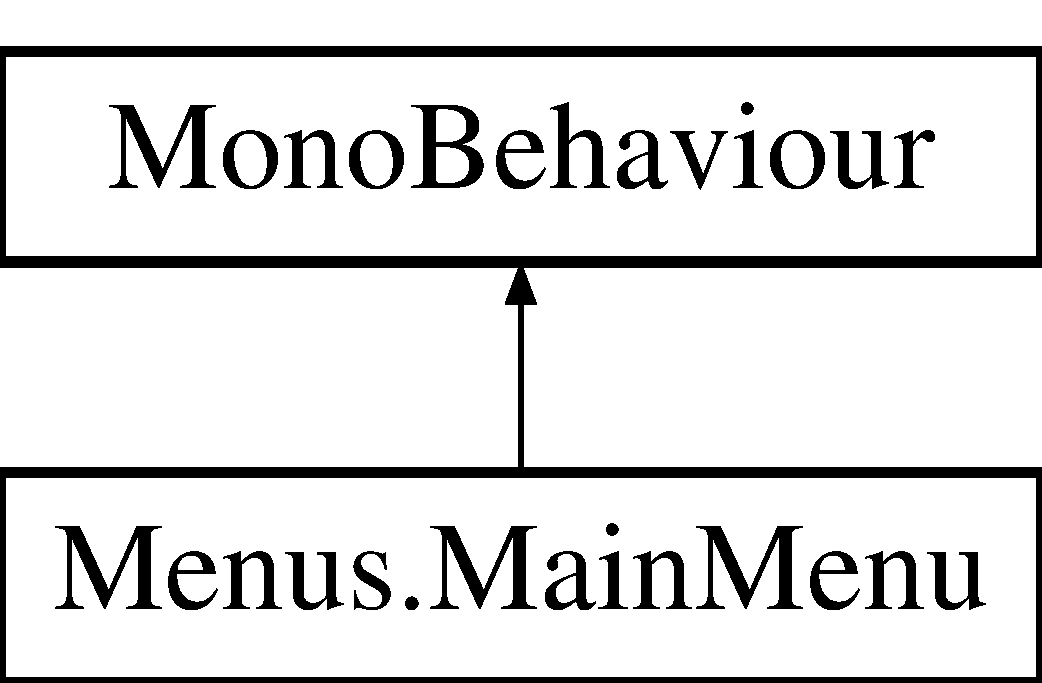
\includegraphics[height=2.000000cm]{class_menus_1_1_main_menu}
\end{center}
\end{figure}
\subsection*{Public Member Functions}
\begin{DoxyCompactItemize}
\item 
void \hyperlink{class_menus_1_1_main_menu_ac97747732432fa983f5a6cb92642df3b}{Start\+Game} ()
\begin{DoxyCompactList}\small\item\em Loads the main game scene \end{DoxyCompactList}\item 
void \hyperlink{class_menus_1_1_main_menu_aa2927bfce459657e7e199a0db8f11d4b}{Open\+High\+Score} ()
\begin{DoxyCompactList}\small\item\em Opens the highscore screen and closes all other open menus \end{DoxyCompactList}\item 
void \hyperlink{class_menus_1_1_main_menu_ae6e4123928bc580afc1469dddd860166}{Open\+Store} ()
\begin{DoxyCompactList}\small\item\em Opens menu for Store \end{DoxyCompactList}\item 
void \hyperlink{class_menus_1_1_main_menu_a3779e5d70d9a7fb549378d6e14709284}{Open} ()
\begin{DoxyCompactList}\small\item\em Opens the menu and closes the others \end{DoxyCompactList}\item 
void {\bfseries Close} ()\hypertarget{class_menus_1_1_main_menu_aea5a4a0bc02f1464a233fed2430d3e32}{}\label{class_menus_1_1_main_menu_aea5a4a0bc02f1464a233fed2430d3e32}

\end{DoxyCompactItemize}


\subsection{Member Function Documentation}
\index{Menus\+::\+Main\+Menu@{Menus\+::\+Main\+Menu}!Open@{Open}}
\index{Open@{Open}!Menus\+::\+Main\+Menu@{Menus\+::\+Main\+Menu}}
\subsubsection[{\texorpdfstring{Open()}{Open()}}]{\setlength{\rightskip}{0pt plus 5cm}void Menus.\+Main\+Menu.\+Open (
\begin{DoxyParamCaption}
{}
\end{DoxyParamCaption}
)\hspace{0.3cm}{\ttfamily [inline]}}\hypertarget{class_menus_1_1_main_menu_a3779e5d70d9a7fb549378d6e14709284}{}\label{class_menus_1_1_main_menu_a3779e5d70d9a7fb549378d6e14709284}


Opens the menu and closes the others 

\index{Menus\+::\+Main\+Menu@{Menus\+::\+Main\+Menu}!Open\+High\+Score@{Open\+High\+Score}}
\index{Open\+High\+Score@{Open\+High\+Score}!Menus\+::\+Main\+Menu@{Menus\+::\+Main\+Menu}}
\subsubsection[{\texorpdfstring{Open\+High\+Score()}{OpenHighScore()}}]{\setlength{\rightskip}{0pt plus 5cm}void Menus.\+Main\+Menu.\+Open\+High\+Score (
\begin{DoxyParamCaption}
{}
\end{DoxyParamCaption}
)\hspace{0.3cm}{\ttfamily [inline]}}\hypertarget{class_menus_1_1_main_menu_aa2927bfce459657e7e199a0db8f11d4b}{}\label{class_menus_1_1_main_menu_aa2927bfce459657e7e199a0db8f11d4b}


Opens the highscore screen and closes all other open menus 

\index{Menus\+::\+Main\+Menu@{Menus\+::\+Main\+Menu}!Open\+Store@{Open\+Store}}
\index{Open\+Store@{Open\+Store}!Menus\+::\+Main\+Menu@{Menus\+::\+Main\+Menu}}
\subsubsection[{\texorpdfstring{Open\+Store()}{OpenStore()}}]{\setlength{\rightskip}{0pt plus 5cm}void Menus.\+Main\+Menu.\+Open\+Store (
\begin{DoxyParamCaption}
{}
\end{DoxyParamCaption}
)\hspace{0.3cm}{\ttfamily [inline]}}\hypertarget{class_menus_1_1_main_menu_ae6e4123928bc580afc1469dddd860166}{}\label{class_menus_1_1_main_menu_ae6e4123928bc580afc1469dddd860166}


Opens menu for Store 

\index{Menus\+::\+Main\+Menu@{Menus\+::\+Main\+Menu}!Start\+Game@{Start\+Game}}
\index{Start\+Game@{Start\+Game}!Menus\+::\+Main\+Menu@{Menus\+::\+Main\+Menu}}
\subsubsection[{\texorpdfstring{Start\+Game()}{StartGame()}}]{\setlength{\rightskip}{0pt plus 5cm}void Menus.\+Main\+Menu.\+Start\+Game (
\begin{DoxyParamCaption}
{}
\end{DoxyParamCaption}
)\hspace{0.3cm}{\ttfamily [inline]}}\hypertarget{class_menus_1_1_main_menu_ac97747732432fa983f5a6cb92642df3b}{}\label{class_menus_1_1_main_menu_ac97747732432fa983f5a6cb92642df3b}


Loads the main game scene 



The documentation for this class was generated from the following file\+:\begin{DoxyCompactItemize}
\item 
Assets/\+Scripts/\+U\+I/Main\+Menu.\+cs\end{DoxyCompactItemize}

\hypertarget{struct_ball_animation_controller_1_1_particle_system_struct}{}\section{Ball\+Animation\+Controller.\+Particle\+System\+Struct Struct Reference}
\label{struct_ball_animation_controller_1_1_particle_system_struct}\index{Ball\+Animation\+Controller.\+Particle\+System\+Struct@{Ball\+Animation\+Controller.\+Particle\+System\+Struct}}


Struct for particle sytems so i don\textquotesingle{}t have to repeat much code  


\subsection*{Public Member Functions}
\begin{DoxyCompactItemize}
\item 
void {\bfseries setup} ()\hypertarget{struct_ball_animation_controller_1_1_particle_system_struct_a176f63ff00ec2d9669eb8b4f11dbc4b6}{}\label{struct_ball_animation_controller_1_1_particle_system_struct_a176f63ff00ec2d9669eb8b4f11dbc4b6}

\end{DoxyCompactItemize}
\subsection*{Public Attributes}
\begin{DoxyCompactItemize}
\item 
bool {\bfseries enabled}\hypertarget{struct_ball_animation_controller_1_1_particle_system_struct_abd3a8ee0586752bb935b16d251ec2bee}{}\label{struct_ball_animation_controller_1_1_particle_system_struct_abd3a8ee0586752bb935b16d251ec2bee}

\item 
Particle\+System {\bfseries System}\hypertarget{struct_ball_animation_controller_1_1_particle_system_struct_a5217c7c96564918afd34d8d01183a9fa}{}\label{struct_ball_animation_controller_1_1_particle_system_struct_a5217c7c96564918afd34d8d01183a9fa}

\item 
Particle\+System.\+Particle\mbox{[}$\,$\mbox{]} {\bfseries Particles}\hypertarget{struct_ball_animation_controller_1_1_particle_system_struct_a294f988f2273cb95ae2ea200cfb8b2ed}{}\label{struct_ball_animation_controller_1_1_particle_system_struct_a294f988f2273cb95ae2ea200cfb8b2ed}

\end{DoxyCompactItemize}


\subsection{Detailed Description}
Struct for particle sytems so i don\textquotesingle{}t have to repeat much code 



The documentation for this struct was generated from the following file\+:\begin{DoxyCompactItemize}
\item 
Assets/\+Scripts/\+Controlers/Ball\+Animation\+Controller.\+cs\end{DoxyCompactItemize}

\hypertarget{class_pause_menu}{}\section{Pause\+Menu Class Reference}
\label{class_pause_menu}\index{Pause\+Menu@{Pause\+Menu}}


Pause Menu Opens when the player pauses the game  


Inheritance diagram for Pause\+Menu\+:\begin{figure}[H]
\begin{center}
\leavevmode
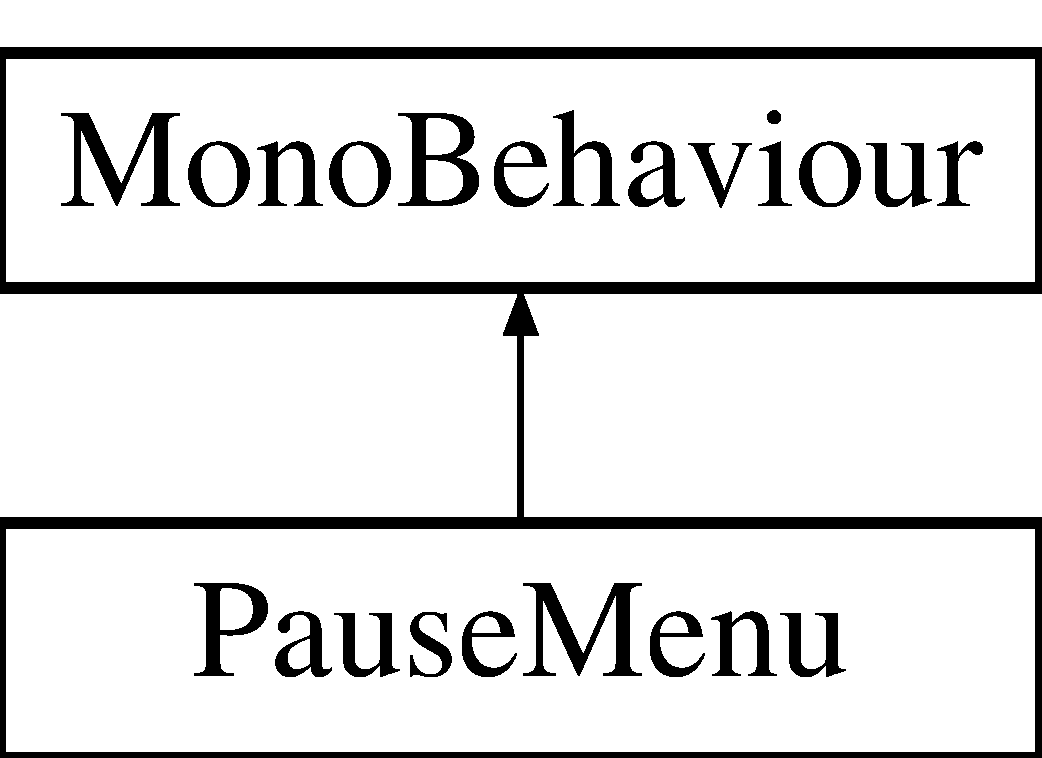
\includegraphics[height=2.000000cm]{class_pause_menu}
\end{center}
\end{figure}
\subsection*{Public Member Functions}
\begin{DoxyCompactItemize}
\item 
void \hyperlink{class_pause_menu_a42be18ab0dceeb064b89799cc808b559}{Close} ()
\begin{DoxyCompactList}\small\item\em Close the pause menu \end{DoxyCompactList}\item 
void {\bfseries On\+Destroy} ()\hypertarget{class_pause_menu_ad2313b208496834e65bbbcabd458e5c2}{}\label{class_pause_menu_ad2313b208496834e65bbbcabd458e5c2}

\item 
void {\bfseries Back\+To\+Main\+Menu} ()\hypertarget{class_pause_menu_a8ac929b22f8ca73cbdf542853485a5a2}{}\label{class_pause_menu_a8ac929b22f8ca73cbdf542853485a5a2}

\end{DoxyCompactItemize}


\subsection{Detailed Description}
Pause Menu Opens when the player pauses the game 



\subsection{Member Function Documentation}
\index{Pause\+Menu@{Pause\+Menu}!Close@{Close}}
\index{Close@{Close}!Pause\+Menu@{Pause\+Menu}}
\subsubsection[{\texorpdfstring{Close()}{Close()}}]{\setlength{\rightskip}{0pt plus 5cm}void Pause\+Menu.\+Close (
\begin{DoxyParamCaption}
{}
\end{DoxyParamCaption}
)\hspace{0.3cm}{\ttfamily [inline]}}\hypertarget{class_pause_menu_a42be18ab0dceeb064b89799cc808b559}{}\label{class_pause_menu_a42be18ab0dceeb064b89799cc808b559}


Close the pause menu 



The documentation for this class was generated from the following file\+:\begin{DoxyCompactItemize}
\item 
Assets/\+Scripts/\+U\+I/Pause\+Menu.\+cs\end{DoxyCompactItemize}

\hypertarget{class_save_data}{}\section{Save\+Data Class Reference}
\label{class_save_data}\index{Save\+Data@{Save\+Data}}
\subsection*{Classes}
\begin{DoxyCompactItemize}
\item 
struct \hyperlink{struct_save_data_1_1_score_block}{Score\+Block}
\end{DoxyCompactItemize}
\subsection*{Public Attributes}
\begin{DoxyCompactItemize}
\item 
\hyperlink{struct_save_data_1_1_score_block}{Score\+Block}\mbox{[}$\,$\mbox{]} {\bfseries high\+Scores}\hypertarget{class_save_data_ad6b597fae588561b2cab802255210781}{}\label{class_save_data_ad6b597fae588561b2cab802255210781}

\item 
bool\mbox{[}$\,$\mbox{]} {\bfseries Unlocked\+Characters} = new bool\mbox{[}0\mbox{]}\hypertarget{class_save_data_af0386c50f7a6c086d961118aa6f80b24}{}\label{class_save_data_af0386c50f7a6c086d961118aa6f80b24}

\item 
bool\mbox{[}$\,$\mbox{]} {\bfseries Unlocked\+Backgrounds} = new bool\mbox{[}0\mbox{]}\hypertarget{class_save_data_a6989ed440d66cee33ae1a8501af3d1be}{}\label{class_save_data_a6989ed440d66cee33ae1a8501af3d1be}

\item 
int {\bfseries Selected\+Character} = 0\hypertarget{class_save_data_a6f8a789b4a102c7ae5038ff8a8c86088}{}\label{class_save_data_a6f8a789b4a102c7ae5038ff8a8c86088}

\item 
int {\bfseries Store\+Points} = 0\hypertarget{class_save_data_a96bd1137583a956bca2e7bd26cd11f89}{}\label{class_save_data_a96bd1137583a956bca2e7bd26cd11f89}

\item 
int {\bfseries Selected\+Background} = 0\hypertarget{class_save_data_afc48c9d7e880061617adfc388800f8bb}{}\label{class_save_data_afc48c9d7e880061617adfc388800f8bb}

\end{DoxyCompactItemize}


The documentation for this class was generated from the following file\+:\begin{DoxyCompactItemize}
\item 
Assets/\+Scripts/Save\+Data.\+cs\end{DoxyCompactItemize}

\hypertarget{class_scale_to_camera_view}{}\section{Scale\+To\+Camera\+View Class Reference}
\label{class_scale_to_camera_view}\index{Scale\+To\+Camera\+View@{Scale\+To\+Camera\+View}}
Inheritance diagram for Scale\+To\+Camera\+View\+:\begin{figure}[H]
\begin{center}
\leavevmode
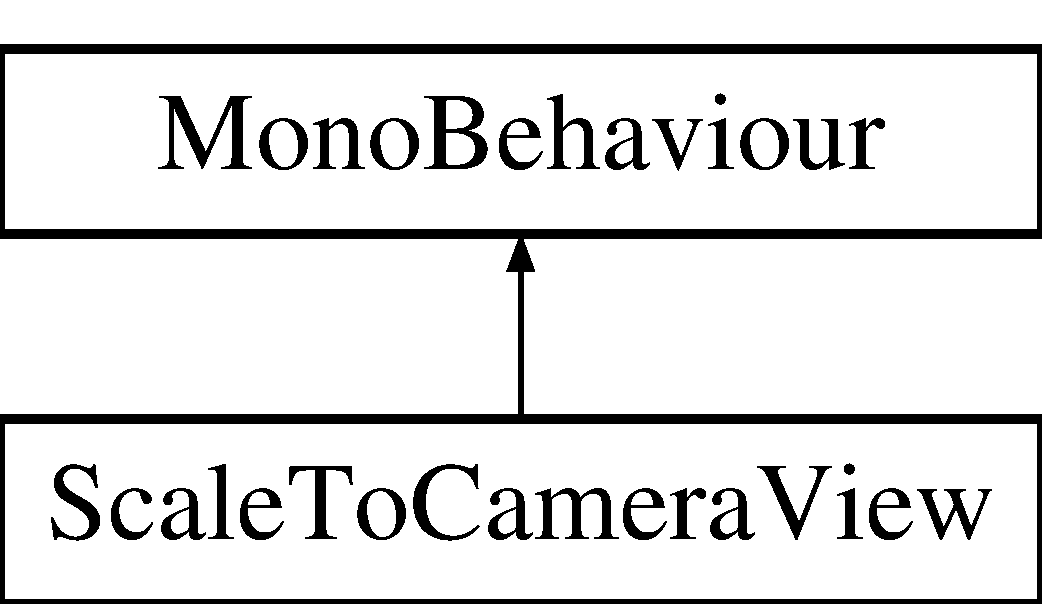
\includegraphics[height=2.000000cm]{class_scale_to_camera_view}
\end{center}
\end{figure}


The documentation for this class was generated from the following file\+:\begin{DoxyCompactItemize}
\item 
Assets/\+Scripts/\+Util/Scale\+To\+Camera\+View.\+cs\end{DoxyCompactItemize}

\hypertarget{class_util_1_1_scale_to_screen_size}{}\section{Util.\+Scale\+To\+Screen\+Size Class Reference}
\label{class_util_1_1_scale_to_screen_size}\index{Util.\+Scale\+To\+Screen\+Size@{Util.\+Scale\+To\+Screen\+Size}}


Scales with screen dimensions  


Inheritance diagram for Util.\+Scale\+To\+Screen\+Size\+:\begin{figure}[H]
\begin{center}
\leavevmode
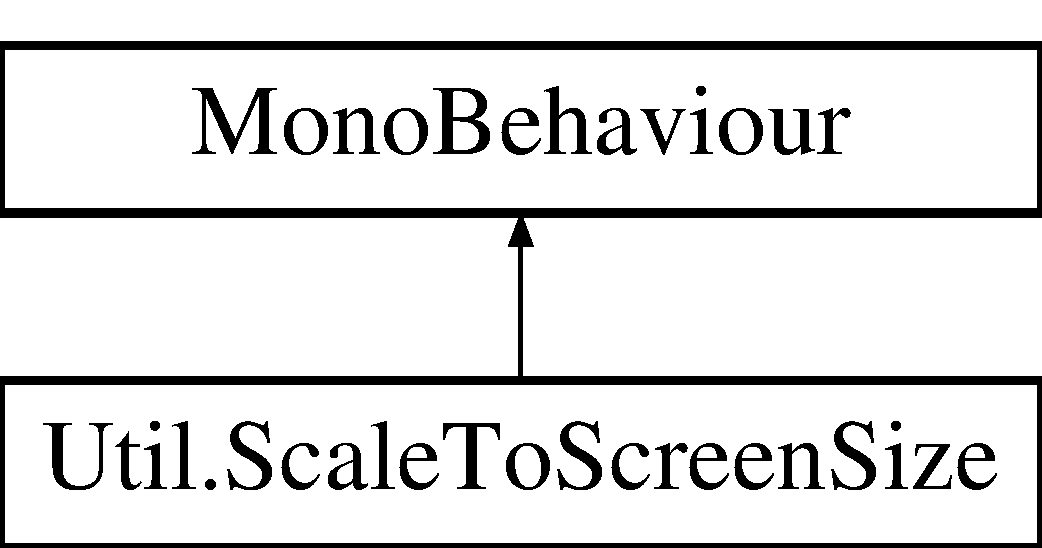
\includegraphics[height=2.000000cm]{class_util_1_1_scale_to_screen_size}
\end{center}
\end{figure}
\subsection*{Public Attributes}
\begin{DoxyCompactItemize}
\item 
Vector3 {\bfseries screen\+Size} = Vector3.\+zero\hypertarget{class_util_1_1_scale_to_screen_size_a6f655c842d9d499f6104a84e8567dbdf}{}\label{class_util_1_1_scale_to_screen_size_a6f655c842d9d499f6104a84e8567dbdf}

\end{DoxyCompactItemize}


\subsection{Detailed Description}
Scales with screen dimensions 



The documentation for this class was generated from the following file\+:\begin{DoxyCompactItemize}
\item 
Assets/\+Scripts/\+Util/Scale\+To\+Screen\+Size.\+cs\end{DoxyCompactItemize}

\hypertarget{class_util_1_1_scene_utils}{}\section{Util.\+Scene\+Utils Class Reference}
\label{class_util_1_1_scene_utils}\index{Util.\+Scene\+Utils@{Util.\+Scene\+Utils}}


Used in quick prototyping of buttons for the UI sytem  


Inheritance diagram for Util.\+Scene\+Utils\+:\begin{figure}[H]
\begin{center}
\leavevmode
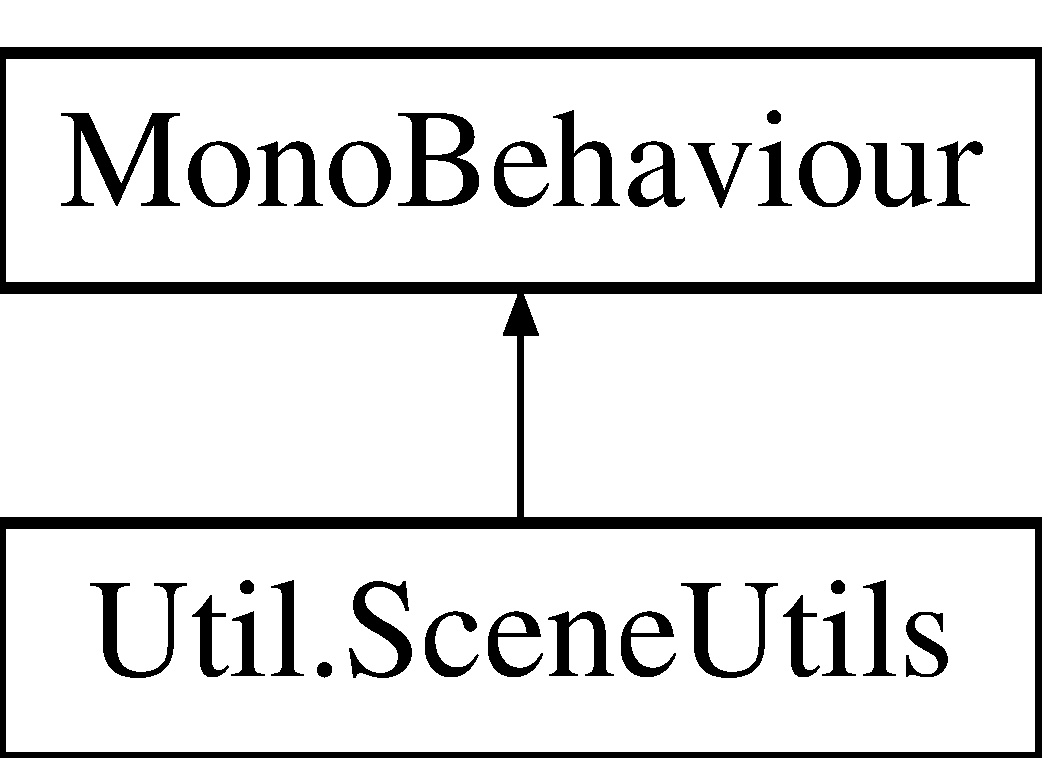
\includegraphics[height=2.000000cm]{class_util_1_1_scene_utils}
\end{center}
\end{figure}
\subsection*{Public Member Functions}
\begin{DoxyCompactItemize}
\item 
void {\bfseries Open\+Scene} (string name)\hypertarget{class_util_1_1_scene_utils_af8e0c852c7dac53b86d44065e5efcdf1}{}\label{class_util_1_1_scene_utils_af8e0c852c7dac53b86d44065e5efcdf1}

\item 
void {\bfseries Close\+Game} ()\hypertarget{class_util_1_1_scene_utils_a51d4e2729e18eedf90b58c463577aa44}{}\label{class_util_1_1_scene_utils_a51d4e2729e18eedf90b58c463577aa44}

\end{DoxyCompactItemize}


\subsection{Detailed Description}
Used in quick prototyping of buttons for the UI sytem 



The documentation for this class was generated from the following file\+:\begin{DoxyCompactItemize}
\item 
Assets/\+Scripts/\+Util/Scene\+Utils.\+cs\end{DoxyCompactItemize}

\hypertarget{struct_save_data_1_1_score_block}{}\section{Save\+Data.\+Score\+Block Struct Reference}
\label{struct_save_data_1_1_score_block}\index{Save\+Data.\+Score\+Block@{Save\+Data.\+Score\+Block}}


Struct that represents a single score in the highscore list  


\subsection*{Public Member Functions}
\begin{DoxyCompactItemize}
\item 
\hyperlink{struct_save_data_1_1_score_block_a3ca084139639f3dce178c7d187315acf}{Score\+Block} (int score, string name)
\begin{DoxyCompactList}\small\item\em Constructor for Scoreblock \end{DoxyCompactList}\end{DoxyCompactItemize}
\subsection*{Public Attributes}
\begin{DoxyCompactItemize}
\item 
int {\bfseries score}\hypertarget{struct_save_data_1_1_score_block_a334fa2ff8427ba7af6989ad28aceea03}{}\label{struct_save_data_1_1_score_block_a334fa2ff8427ba7af6989ad28aceea03}

\item 
string {\bfseries name}\hypertarget{struct_save_data_1_1_score_block_abd747ee96d8c50126232fe3d33b12682}{}\label{struct_save_data_1_1_score_block_abd747ee96d8c50126232fe3d33b12682}

\end{DoxyCompactItemize}


\subsection{Detailed Description}
Struct that represents a single score in the highscore list 



\subsection{Constructor \& Destructor Documentation}
\index{Save\+Data\+::\+Score\+Block@{Save\+Data\+::\+Score\+Block}!Score\+Block@{Score\+Block}}
\index{Score\+Block@{Score\+Block}!Save\+Data\+::\+Score\+Block@{Save\+Data\+::\+Score\+Block}}
\subsubsection[{\texorpdfstring{Score\+Block(int score, string name)}{ScoreBlock(int score, string name)}}]{\setlength{\rightskip}{0pt plus 5cm}Save\+Data.\+Score\+Block.\+Score\+Block (
\begin{DoxyParamCaption}
\item[{int}]{score, }
\item[{string}]{name}
\end{DoxyParamCaption}
)\hspace{0.3cm}{\ttfamily [inline]}}\hypertarget{struct_save_data_1_1_score_block_a3ca084139639f3dce178c7d187315acf}{}\label{struct_save_data_1_1_score_block_a3ca084139639f3dce178c7d187315acf}


Constructor for Scoreblock 


\begin{DoxyParams}{Parameters}
{\em score} & Points scored that the player got durring there run\\
\hline
{\em name} & Name the player gave up when submitting there score to the highscore table\\
\hline
\end{DoxyParams}


The documentation for this struct was generated from the following file\+:\begin{DoxyCompactItemize}
\item 
Assets/\+Scripts/Save\+Data.\+cs\end{DoxyCompactItemize}

\hypertarget{class_util_1_1_serializable_dictionary}{}\section{Util.\+Serializable\+Dictionary$<$ T\+Key, T\+Val $>$ Class Template Reference}
\label{class_util_1_1_serializable_dictionary}\index{Util.\+Serializable\+Dictionary$<$ T\+Key, T\+Val $>$@{Util.\+Serializable\+Dictionary$<$ T\+Key, T\+Val $>$}}
Inheritance diagram for Util.\+Serializable\+Dictionary$<$ T\+Key, T\+Val $>$\+:\begin{figure}[H]
\begin{center}
\leavevmode
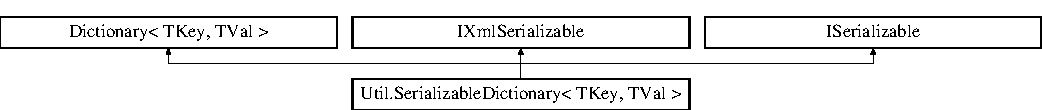
\includegraphics[height=1.475626cm]{class_util_1_1_serializable_dictionary}
\end{center}
\end{figure}
\subsection*{Public Member Functions}
\begin{DoxyCompactItemize}
\item 
{\bfseries Serializable\+Dictionary} (I\+Dictionary$<$ T\+Key, T\+Val $>$ dictionary)\hypertarget{class_util_1_1_serializable_dictionary_a9b3df5a4db46f4bdd84a98bcfd29e7d5}{}\label{class_util_1_1_serializable_dictionary_a9b3df5a4db46f4bdd84a98bcfd29e7d5}

\item 
{\bfseries Serializable\+Dictionary} (I\+Equality\+Comparer$<$ T\+Key $>$ comparer)\hypertarget{class_util_1_1_serializable_dictionary_aebd85fe37168589c3dff359661604e3e}{}\label{class_util_1_1_serializable_dictionary_aebd85fe37168589c3dff359661604e3e}

\item 
{\bfseries Serializable\+Dictionary} (int capacity)\hypertarget{class_util_1_1_serializable_dictionary_a43761f5b4b10f2f19d9a0678fdf942b8}{}\label{class_util_1_1_serializable_dictionary_a43761f5b4b10f2f19d9a0678fdf942b8}

\item 
{\bfseries Serializable\+Dictionary} (I\+Dictionary$<$ T\+Key, T\+Val $>$ dictionary, I\+Equality\+Comparer$<$ T\+Key $>$ comparer)\hypertarget{class_util_1_1_serializable_dictionary_aac656cb4391481872fab36494414beb9}{}\label{class_util_1_1_serializable_dictionary_aac656cb4391481872fab36494414beb9}

\item 
{\bfseries Serializable\+Dictionary} (int capacity, I\+Equality\+Comparer$<$ T\+Key $>$ comparer)\hypertarget{class_util_1_1_serializable_dictionary_a4d263d5213de95a101c07de78fe9cb66}{}\label{class_util_1_1_serializable_dictionary_a4d263d5213de95a101c07de78fe9cb66}

\end{DoxyCompactItemize}
\subsection*{Protected Member Functions}
\begin{DoxyCompactItemize}
\item 
{\bfseries Serializable\+Dictionary} (Serialization\+Info info, Streaming\+Context context)\hypertarget{class_util_1_1_serializable_dictionary_a4cee20b244c018189699e27424a4772d}{}\label{class_util_1_1_serializable_dictionary_a4cee20b244c018189699e27424a4772d}

\end{DoxyCompactItemize}
\subsection*{Properties}
\begin{DoxyCompactItemize}
\item 
Xml\+Serializer {\bfseries Value\+Serializer}\hspace{0.3cm}{\ttfamily  \mbox{[}get\mbox{]}}\hypertarget{class_util_1_1_serializable_dictionary_a25936f4835bc2b4ec1695489a4a17a69}{}\label{class_util_1_1_serializable_dictionary_a25936f4835bc2b4ec1695489a4a17a69}

\end{DoxyCompactItemize}


The documentation for this class was generated from the following file\+:\begin{DoxyCompactItemize}
\item 
Assets/\+Scripts/\+Util/\+Saving/Serializable\+Dictionary.\+cs\end{DoxyCompactItemize}

\hypertarget{class_menus_1_1_shop_menu}{}\section{Menus.\+Shop\+Menu Class Reference}
\label{class_menus_1_1_shop_menu}\index{Menus.\+Shop\+Menu@{Menus.\+Shop\+Menu}}
Inheritance diagram for Menus.\+Shop\+Menu\+:\begin{figure}[H]
\begin{center}
\leavevmode
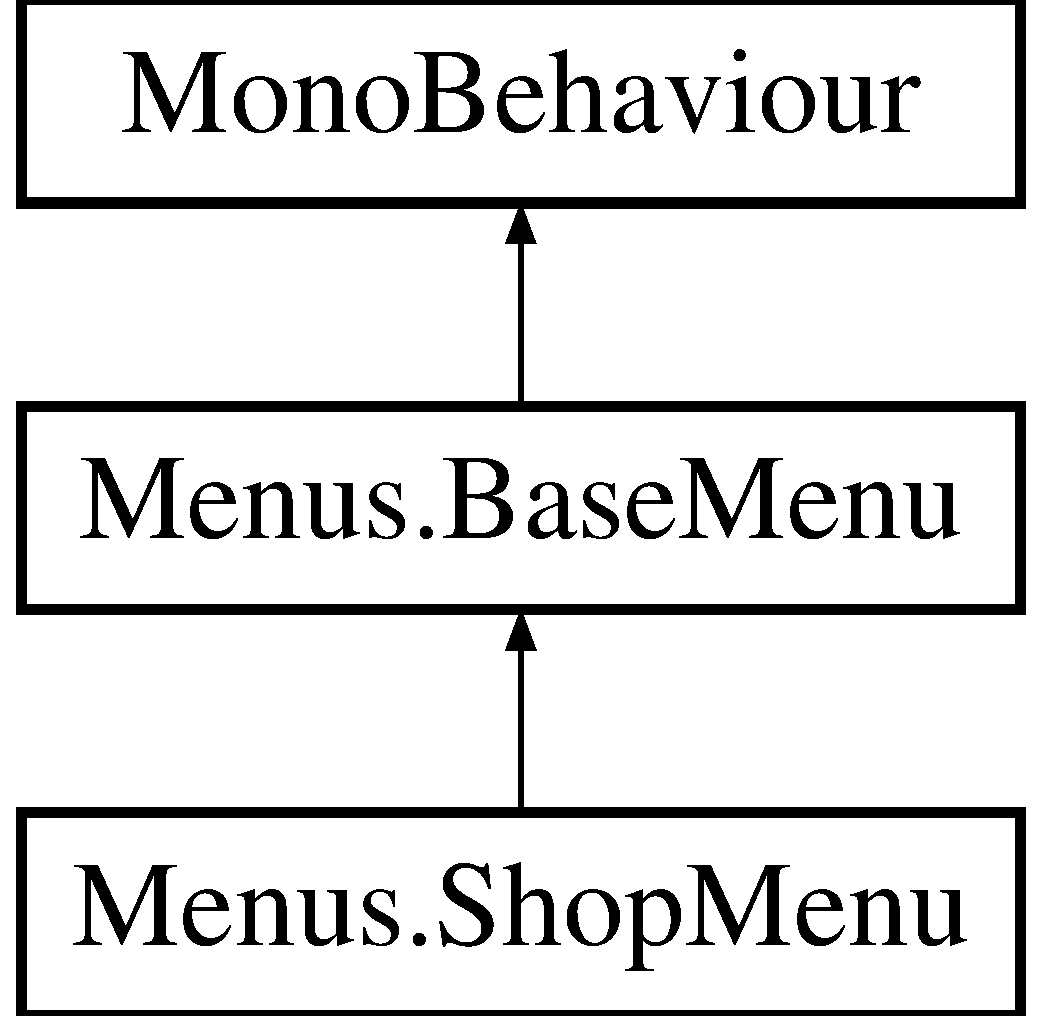
\includegraphics[height=3.000000cm]{class_menus_1_1_shop_menu}
\end{center}
\end{figure}
\subsection*{Public Member Functions}
\begin{DoxyCompactItemize}
\item 
override void \hyperlink{class_menus_1_1_shop_menu_af79b153c30d06137091f0b021d2c626b}{Open} ()
\begin{DoxyCompactList}\small\item\em Open menu \end{DoxyCompactList}\item 
void \hyperlink{class_menus_1_1_shop_menu_a73ccd36ee27ff79f736fc7aa563d1cc1}{Open\+Character} ()
\begin{DoxyCompactList}\small\item\em Opens character selection menu \end{DoxyCompactList}\item 
void \hyperlink{class_menus_1_1_shop_menu_a903ec61aa167d426010e4632ec9e3f59}{Open\+Backgrounds} ()
\begin{DoxyCompactList}\small\item\em Opens background selection menu \end{DoxyCompactList}\item 
void \hyperlink{class_menus_1_1_shop_menu_a403a38bf336dacd0d5f412ba0aaf4520}{Click\+Character} (int Index)
\begin{DoxyCompactList}\small\item\em Handels clicks on a character and checks if it has been unlocked and if it is then it will select that character Else \end{DoxyCompactList}\item 
void \hyperlink{class_menus_1_1_shop_menu_a8aa4cb8db5ba4c53087af77e39232cf6}{Click\+Background} (int Index)
\begin{DoxyCompactList}\small\item\em Handels Clicks for the Backgrounds. Also checks if a background as been unlocked \end{DoxyCompactList}\end{DoxyCompactItemize}
\subsection*{Additional Inherited Members}


\subsection{Member Function Documentation}
\index{Menus\+::\+Shop\+Menu@{Menus\+::\+Shop\+Menu}!Click\+Background@{Click\+Background}}
\index{Click\+Background@{Click\+Background}!Menus\+::\+Shop\+Menu@{Menus\+::\+Shop\+Menu}}
\subsubsection[{\texorpdfstring{Click\+Background(int Index)}{ClickBackground(int Index)}}]{\setlength{\rightskip}{0pt plus 5cm}void Menus.\+Shop\+Menu.\+Click\+Background (
\begin{DoxyParamCaption}
\item[{int}]{Index}
\end{DoxyParamCaption}
)\hspace{0.3cm}{\ttfamily [inline]}}\hypertarget{class_menus_1_1_shop_menu_a8aa4cb8db5ba4c53087af77e39232cf6}{}\label{class_menus_1_1_shop_menu_a8aa4cb8db5ba4c53087af77e39232cf6}


Handels Clicks for the Backgrounds. Also checks if a background as been unlocked 


\begin{DoxyParams}{Parameters}
{\em Index} & Index of the item that was clicked on\\
\hline
\end{DoxyParams}
\index{Menus\+::\+Shop\+Menu@{Menus\+::\+Shop\+Menu}!Click\+Character@{Click\+Character}}
\index{Click\+Character@{Click\+Character}!Menus\+::\+Shop\+Menu@{Menus\+::\+Shop\+Menu}}
\subsubsection[{\texorpdfstring{Click\+Character(int Index)}{ClickCharacter(int Index)}}]{\setlength{\rightskip}{0pt plus 5cm}void Menus.\+Shop\+Menu.\+Click\+Character (
\begin{DoxyParamCaption}
\item[{int}]{Index}
\end{DoxyParamCaption}
)\hspace{0.3cm}{\ttfamily [inline]}}\hypertarget{class_menus_1_1_shop_menu_a403a38bf336dacd0d5f412ba0aaf4520}{}\label{class_menus_1_1_shop_menu_a403a38bf336dacd0d5f412ba0aaf4520}


Handels clicks on a character and checks if it has been unlocked and if it is then it will select that character Else 


\begin{DoxyParams}{Parameters}
{\em Index} & Index of the item that clicked\\
\hline
\end{DoxyParams}
\index{Menus\+::\+Shop\+Menu@{Menus\+::\+Shop\+Menu}!Open@{Open}}
\index{Open@{Open}!Menus\+::\+Shop\+Menu@{Menus\+::\+Shop\+Menu}}
\subsubsection[{\texorpdfstring{Open()}{Open()}}]{\setlength{\rightskip}{0pt plus 5cm}override void Menus.\+Shop\+Menu.\+Open (
\begin{DoxyParamCaption}
{}
\end{DoxyParamCaption}
)\hspace{0.3cm}{\ttfamily [inline]}, {\ttfamily [virtual]}}\hypertarget{class_menus_1_1_shop_menu_af79b153c30d06137091f0b021d2c626b}{}\label{class_menus_1_1_shop_menu_af79b153c30d06137091f0b021d2c626b}


Open menu 

by default it just enables and disables the game object 

Reimplemented from \hyperlink{class_menus_1_1_base_menu_aedf5a0abb1c46b9687cba0f216734176}{Menus.\+Base\+Menu}.

\index{Menus\+::\+Shop\+Menu@{Menus\+::\+Shop\+Menu}!Open\+Backgrounds@{Open\+Backgrounds}}
\index{Open\+Backgrounds@{Open\+Backgrounds}!Menus\+::\+Shop\+Menu@{Menus\+::\+Shop\+Menu}}
\subsubsection[{\texorpdfstring{Open\+Backgrounds()}{OpenBackgrounds()}}]{\setlength{\rightskip}{0pt plus 5cm}void Menus.\+Shop\+Menu.\+Open\+Backgrounds (
\begin{DoxyParamCaption}
{}
\end{DoxyParamCaption}
)\hspace{0.3cm}{\ttfamily [inline]}}\hypertarget{class_menus_1_1_shop_menu_a903ec61aa167d426010e4632ec9e3f59}{}\label{class_menus_1_1_shop_menu_a903ec61aa167d426010e4632ec9e3f59}


Opens background selection menu 

\index{Menus\+::\+Shop\+Menu@{Menus\+::\+Shop\+Menu}!Open\+Character@{Open\+Character}}
\index{Open\+Character@{Open\+Character}!Menus\+::\+Shop\+Menu@{Menus\+::\+Shop\+Menu}}
\subsubsection[{\texorpdfstring{Open\+Character()}{OpenCharacter()}}]{\setlength{\rightskip}{0pt plus 5cm}void Menus.\+Shop\+Menu.\+Open\+Character (
\begin{DoxyParamCaption}
{}
\end{DoxyParamCaption}
)\hspace{0.3cm}{\ttfamily [inline]}}\hypertarget{class_menus_1_1_shop_menu_a73ccd36ee27ff79f736fc7aa563d1cc1}{}\label{class_menus_1_1_shop_menu_a73ccd36ee27ff79f736fc7aa563d1cc1}


Opens character selection menu 



The documentation for this class was generated from the following file\+:\begin{DoxyCompactItemize}
\item 
Assets/\+Scripts/\+U\+I/\+Shop\+Menu/Shop\+Menu.\+cs\end{DoxyCompactItemize}

\hypertarget{class_menus_1_1_shop_menu_data}{}\section{Menus.\+Shop\+Menu\+Data Class Reference}
\label{class_menus_1_1_shop_menu_data}\index{Menus.\+Shop\+Menu\+Data@{Menus.\+Shop\+Menu\+Data}}
Inheritance diagram for Menus.\+Shop\+Menu\+Data\+:\begin{figure}[H]
\begin{center}
\leavevmode
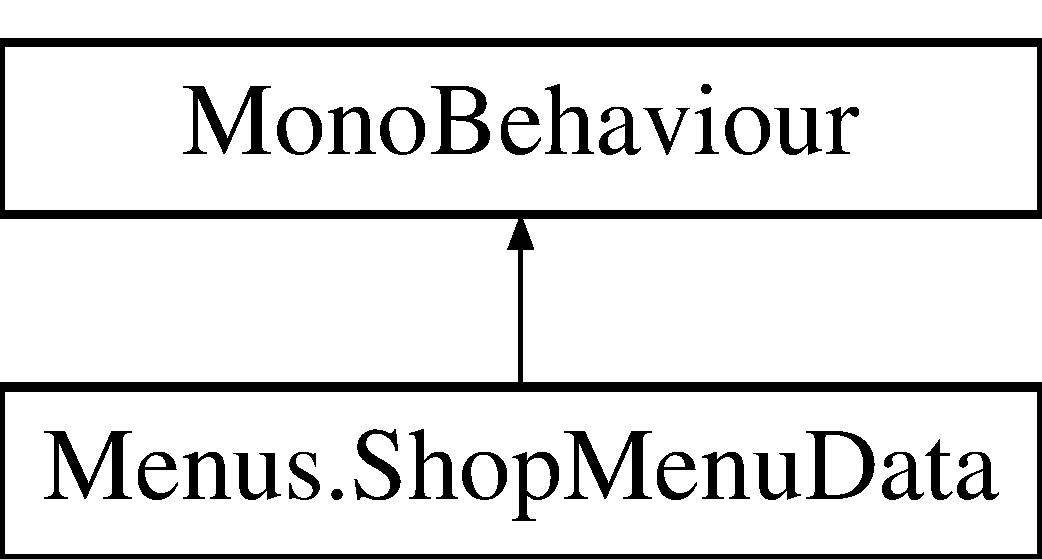
\includegraphics[height=2.000000cm]{class_menus_1_1_shop_menu_data}
\end{center}
\end{figure}
\subsection*{Classes}
\begin{DoxyCompactItemize}
\item 
struct \hyperlink{struct_menus_1_1_shop_menu_data_1_1_store_object}{Store\+Object}
\end{DoxyCompactItemize}
\subsection*{Public Attributes}
\begin{DoxyCompactItemize}
\item 
const string {\bfseries Resource\+Name} = \char`\"{}Shop\+Data\char`\"{}\hypertarget{class_menus_1_1_shop_menu_data_a0f1c9a23c1e5da1011eacc742121334a}{}\label{class_menus_1_1_shop_menu_data_a0f1c9a23c1e5da1011eacc742121334a}

\end{DoxyCompactItemize}
\subsection*{Properties}
\begin{DoxyCompactItemize}
\item 
\hyperlink{struct_menus_1_1_shop_menu_data_1_1_store_object}{Store\+Object}\mbox{[}$\,$\mbox{]} {\bfseries Characters}\hspace{0.3cm}{\ttfamily  \mbox{[}get\mbox{]}}\hypertarget{class_menus_1_1_shop_menu_data_abbc6902ebe3cb79170943783e5a25415}{}\label{class_menus_1_1_shop_menu_data_abbc6902ebe3cb79170943783e5a25415}

\item 
\hyperlink{struct_menus_1_1_shop_menu_data_1_1_store_object}{Store\+Object}\mbox{[}$\,$\mbox{]} {\bfseries Backgrounds}\hspace{0.3cm}{\ttfamily  \mbox{[}get\mbox{]}}\hypertarget{class_menus_1_1_shop_menu_data_a7736493b49a50ab592f5772933fa0ce9}{}\label{class_menus_1_1_shop_menu_data_a7736493b49a50ab592f5772933fa0ce9}

\end{DoxyCompactItemize}


The documentation for this class was generated from the following file\+:\begin{DoxyCompactItemize}
\item 
Assets/\+Scripts/\+U\+I/\+Shop\+Menu/Shop\+Menu\+Data.\+cs\end{DoxyCompactItemize}

\hypertarget{class_util_1_1_slider_setter}{}\section{Util.\+Slider\+Setter Class Reference}
\label{class_util_1_1_slider_setter}\index{Util.\+Slider\+Setter@{Util.\+Slider\+Setter}}
Inheritance diagram for Util.\+Slider\+Setter\+:\begin{figure}[H]
\begin{center}
\leavevmode
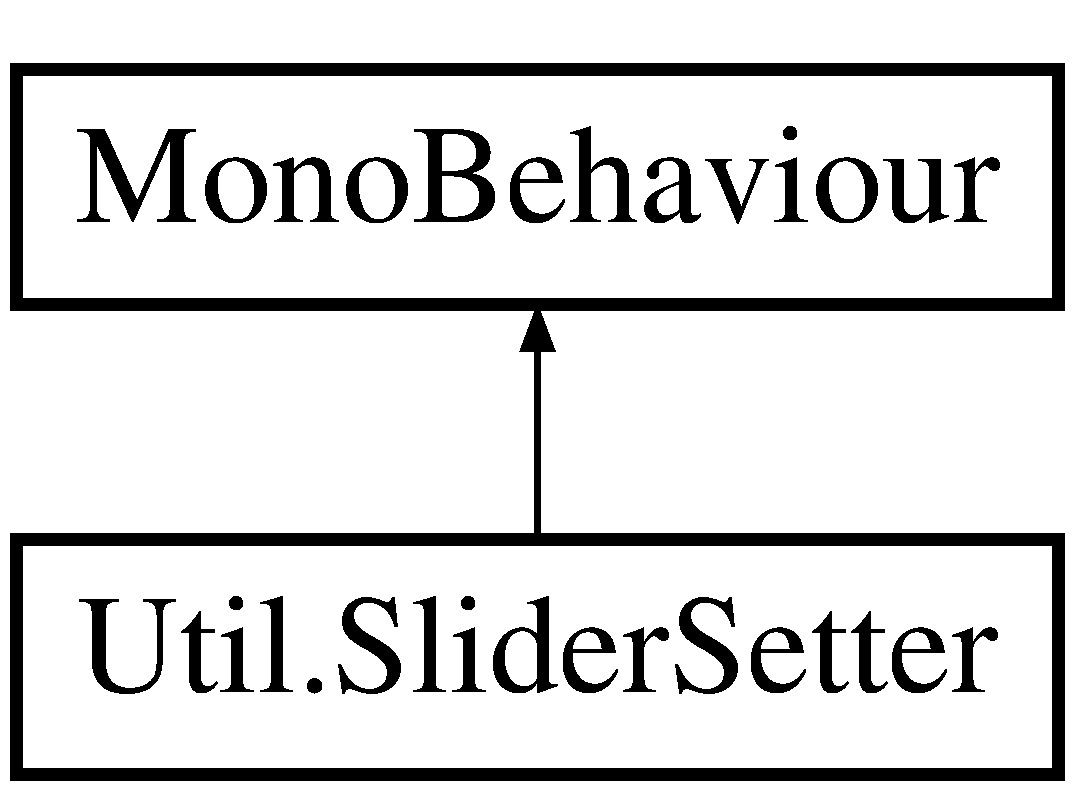
\includegraphics[height=2.000000cm]{class_util_1_1_slider_setter}
\end{center}
\end{figure}
\subsection*{Public Attributes}
\begin{DoxyCompactItemize}
\item 
Slider {\bfseries slider}\hypertarget{class_util_1_1_slider_setter_a62cd8a868eabb986ab3207035ec40267}{}\label{class_util_1_1_slider_setter_a62cd8a868eabb986ab3207035ec40267}

\item 
Scroll\+Rect {\bfseries scroll\+Rect}\hypertarget{class_util_1_1_slider_setter_a3caf6d33b16290ff116a131dad12104a}{}\label{class_util_1_1_slider_setter_a3caf6d33b16290ff116a131dad12104a}

\item 
float {\bfseries Start\+Value}\hypertarget{class_util_1_1_slider_setter_a0df4f45f646465e46667bcac0b6ef2e5}{}\label{class_util_1_1_slider_setter_a0df4f45f646465e46667bcac0b6ef2e5}

\end{DoxyCompactItemize}


The documentation for this class was generated from the following file\+:\begin{DoxyCompactItemize}
\item 
Assets/\+Scripts/\+Util/Slider\+Setter.\+cs\end{DoxyCompactItemize}

\hypertarget{class_snap_to_screen_point}{}\section{Snap\+To\+Screen\+Point Class Reference}
\label{class_snap_to_screen_point}\index{Snap\+To\+Screen\+Point@{Snap\+To\+Screen\+Point}}
Inheritance diagram for Snap\+To\+Screen\+Point\+:\begin{figure}[H]
\begin{center}
\leavevmode
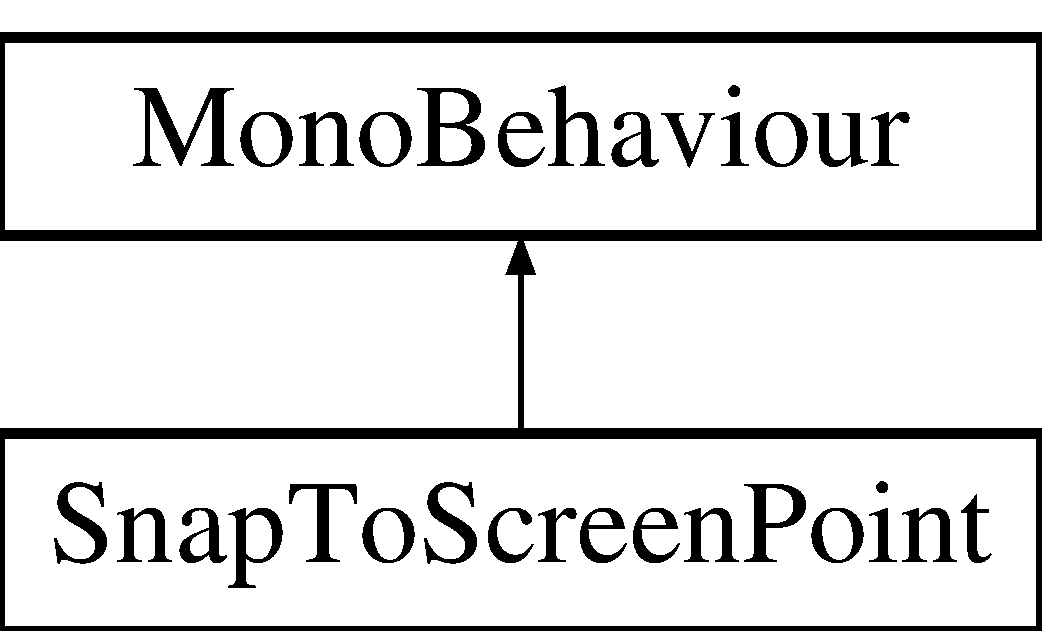
\includegraphics[height=2.000000cm]{class_snap_to_screen_point}
\end{center}
\end{figure}
\subsection*{Public Attributes}
\begin{DoxyCompactItemize}
\item 
Vector3 {\bfseries screen\+Position} = Vector3.\+zero\hypertarget{class_snap_to_screen_point_af16a0e4b3b605f83f8382f759b7e2ef4}{}\label{class_snap_to_screen_point_af16a0e4b3b605f83f8382f759b7e2ef4}

\item 
Vector2 {\bfseries Start\+Size} = Vector2.\+one\hypertarget{class_snap_to_screen_point_a1c894fdec5879ad749eb2a0fb86c4637}{}\label{class_snap_to_screen_point_a1c894fdec5879ad749eb2a0fb86c4637}

\end{DoxyCompactItemize}


The documentation for this class was generated from the following file\+:\begin{DoxyCompactItemize}
\item 
Assets/\+Scripts/\+Util/Snap\+To\+Screen\+Point.\+cs\end{DoxyCompactItemize}

\hypertarget{class_splash_screen}{}\section{Splash\+Screen Class Reference}
\label{class_splash_screen}\index{Splash\+Screen@{Splash\+Screen}}
Inheritance diagram for Splash\+Screen\+:\begin{figure}[H]
\begin{center}
\leavevmode
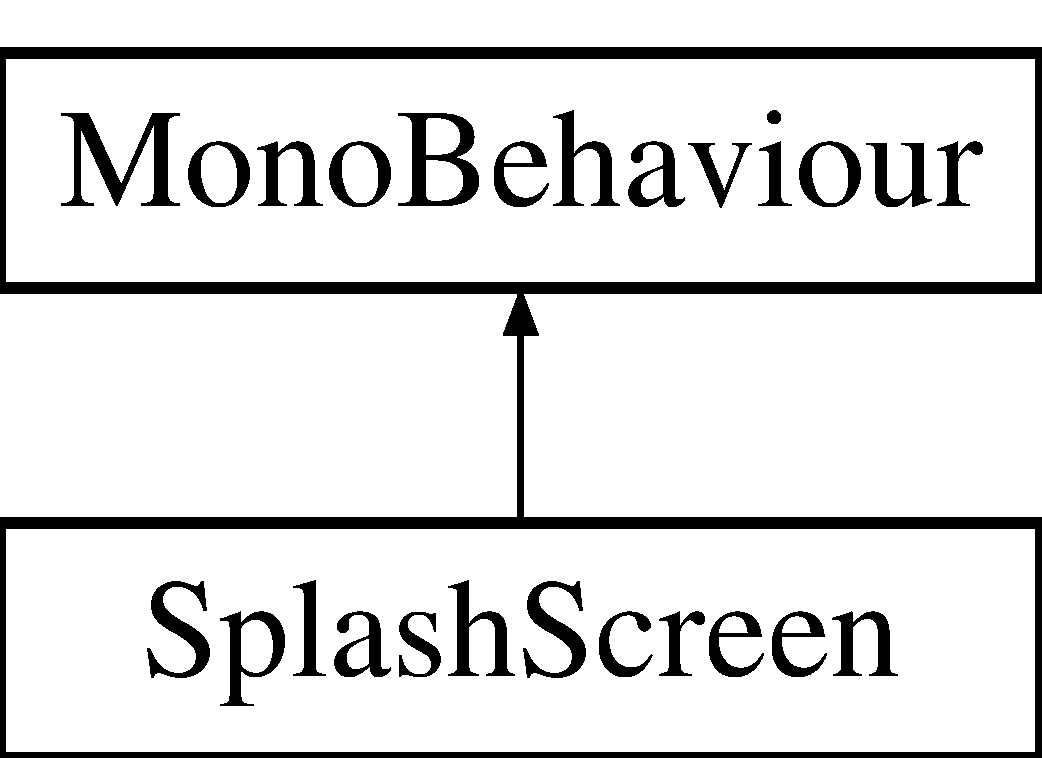
\includegraphics[height=2.000000cm]{class_splash_screen}
\end{center}
\end{figure}


The documentation for this class was generated from the following file\+:\begin{DoxyCompactItemize}
\item 
Assets/\+Scripts/Splash\+Screen.\+cs\end{DoxyCompactItemize}

\hypertarget{class_menus_1_1_shop_menu_data_1_1_store_object}{}\section{Menus.\+Shop\+Menu\+Data.\+Store\+Object Class Reference}
\label{class_menus_1_1_shop_menu_data_1_1_store_object}\index{Menus.\+Shop\+Menu\+Data.\+Store\+Object@{Menus.\+Shop\+Menu\+Data.\+Store\+Object}}


Base store object contains a name and a cost of the object  


Inheritance diagram for Menus.\+Shop\+Menu\+Data.\+Store\+Object\+:\begin{figure}[H]
\begin{center}
\leavevmode
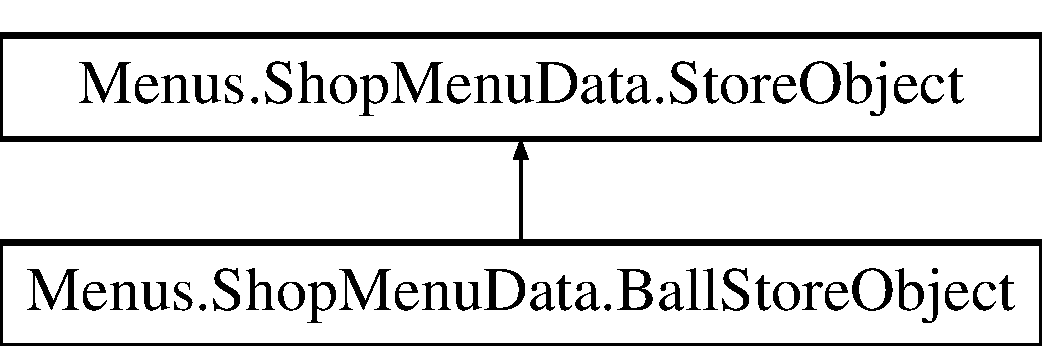
\includegraphics[height=2.000000cm]{class_menus_1_1_shop_menu_data_1_1_store_object}
\end{center}
\end{figure}
\subsection*{Public Attributes}
\begin{DoxyCompactItemize}
\item 
int {\bfseries Cost}\hypertarget{class_menus_1_1_shop_menu_data_1_1_store_object_a7a7b36b71c978cb11dda711ea66f7eb3}{}\label{class_menus_1_1_shop_menu_data_1_1_store_object_a7a7b36b71c978cb11dda711ea66f7eb3}

\item 
string {\bfseries Name}\hypertarget{class_menus_1_1_shop_menu_data_1_1_store_object_ae8a3658a4964a9a67b1de0fbee128869}{}\label{class_menus_1_1_shop_menu_data_1_1_store_object_ae8a3658a4964a9a67b1de0fbee128869}

\end{DoxyCompactItemize}
\subsection*{Properties}
\begin{DoxyCompactItemize}
\item 
Sprite {\bfseries High\+Res}\hspace{0.3cm}{\ttfamily  \mbox{[}get\mbox{]}}\hypertarget{class_menus_1_1_shop_menu_data_1_1_store_object_a14be1f6f44cedb1b46260ffe9197f856}{}\label{class_menus_1_1_shop_menu_data_1_1_store_object_a14be1f6f44cedb1b46260ffe9197f856}

\item 
Sprite {\bfseries Low\+Res}\hspace{0.3cm}{\ttfamily  \mbox{[}get\mbox{]}}\hypertarget{class_menus_1_1_shop_menu_data_1_1_store_object_af86650045d1d10d13bb22246b92e0a2e}{}\label{class_menus_1_1_shop_menu_data_1_1_store_object_af86650045d1d10d13bb22246b92e0a2e}

\end{DoxyCompactItemize}


\subsection{Detailed Description}
Base store object contains a name and a cost of the object 



The documentation for this class was generated from the following file\+:\begin{DoxyCompactItemize}
\item 
Assets/\+Scripts/\+U\+I/\+Shop\+Menu/Shop\+Menu\+Data.\+cs\end{DoxyCompactItemize}

\hypertarget{class_target_controller}{}\section{Target\+Controller Class Reference}
\label{class_target_controller}\index{Target\+Controller@{Target\+Controller}}
Inheritance diagram for Target\+Controller\+:\begin{figure}[H]
\begin{center}
\leavevmode
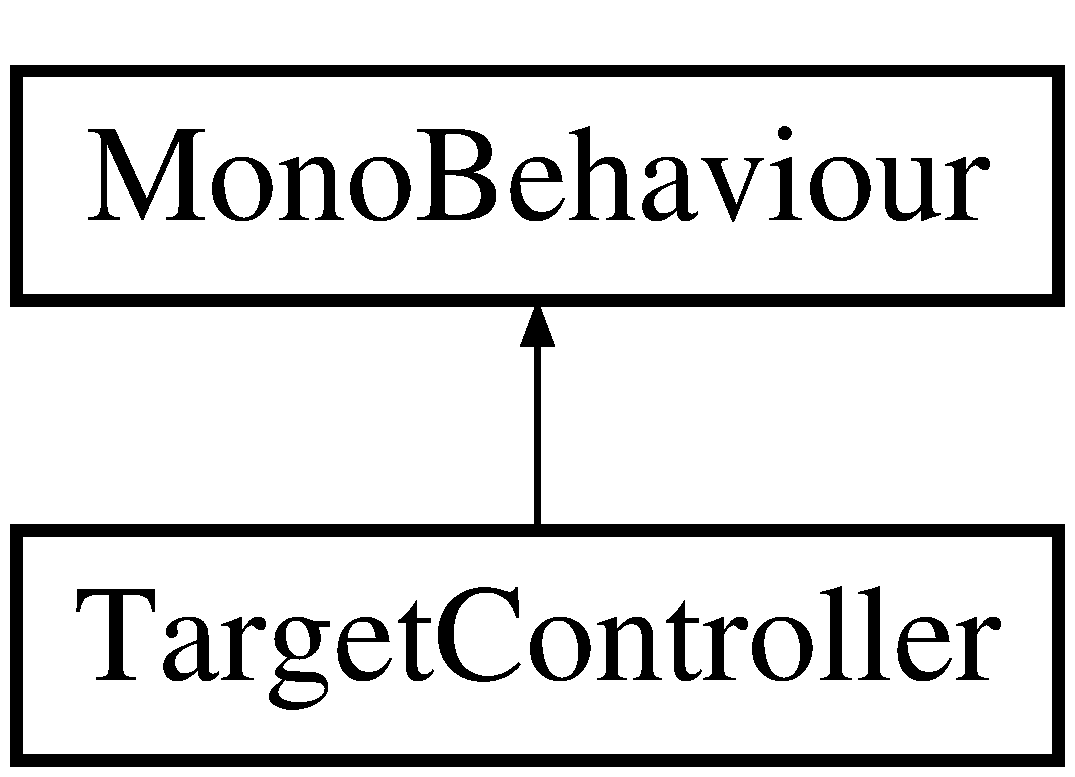
\includegraphics[height=2.000000cm]{class_target_controller}
\end{center}
\end{figure}
\subsection*{Public Member Functions}
\begin{DoxyCompactItemize}
\item 
void {\bfseries On\+Destroy} ()\hypertarget{class_target_controller_a3f8c8d02ceb9fedeff04f8edf2f9a63d}{}\label{class_target_controller_a3f8c8d02ceb9fedeff04f8edf2f9a63d}

\end{DoxyCompactItemize}


The documentation for this class was generated from the following file\+:\begin{DoxyCompactItemize}
\item 
Assets/\+Scripts/\+Controlers/Target\+Controller.\+cs\end{DoxyCompactItemize}

\hypertarget{class_u_i_manager}{}\section{U\+I\+Manager Class Reference}
\label{class_u_i_manager}\index{U\+I\+Manager@{U\+I\+Manager}}


Controles the ingame UI  


Inheritance diagram for U\+I\+Manager\+:\begin{figure}[H]
\begin{center}
\leavevmode
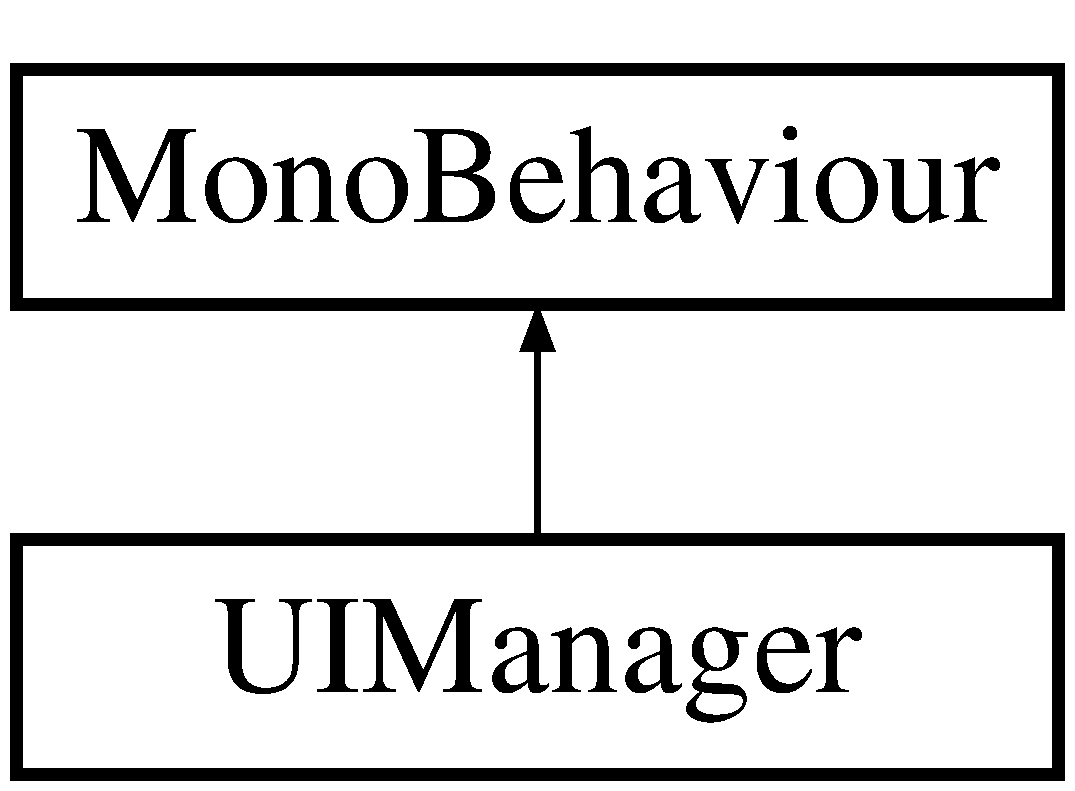
\includegraphics[height=2.000000cm]{class_u_i_manager}
\end{center}
\end{figure}
\subsection*{Public Member Functions}
\begin{DoxyCompactItemize}
\item 
void {\bfseries On\+Destroy} ()\hypertarget{class_u_i_manager_a03255ab474c26f8da63d87821decd3e1}{}\label{class_u_i_manager_a03255ab474c26f8da63d87821decd3e1}

\end{DoxyCompactItemize}


\subsection{Detailed Description}
Controles the ingame UI 



The documentation for this class was generated from the following file\+:\begin{DoxyCompactItemize}
\item 
Assets/\+Scripts/\+Managers/U\+I\+Manager.\+cs\end{DoxyCompactItemize}

\hypertarget{class_util_1_1_value_debugger}{}\section{Util.\+Value\+Debugger Class Reference}
\label{class_util_1_1_value_debugger}\index{Util.\+Value\+Debugger@{Util.\+Value\+Debugger}}
Inheritance diagram for Util.\+Value\+Debugger\+:\begin{figure}[H]
\begin{center}
\leavevmode
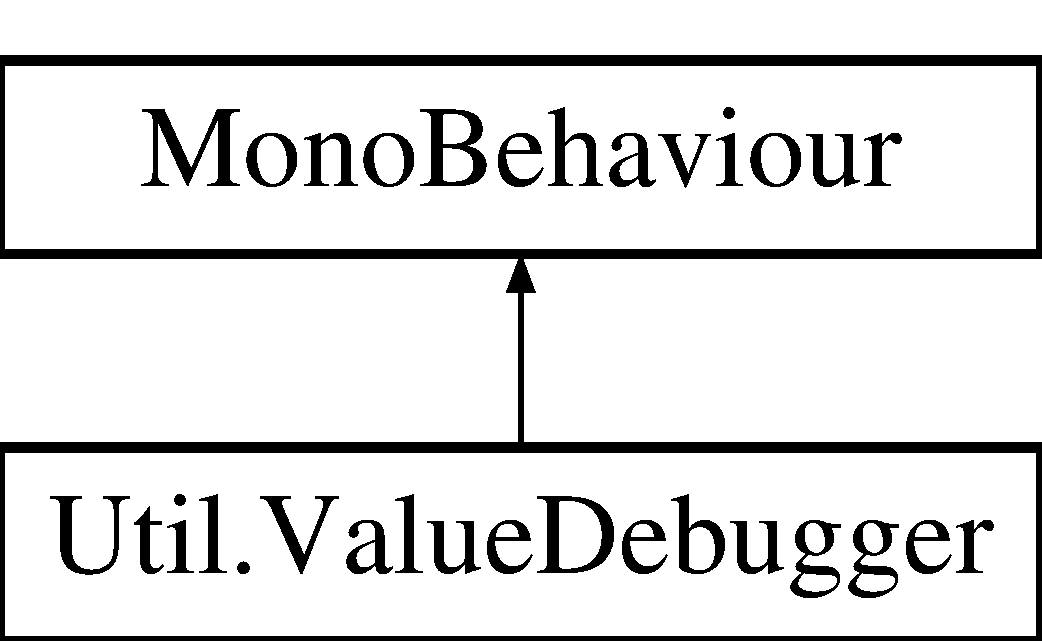
\includegraphics[height=2.000000cm]{class_util_1_1_value_debugger}
\end{center}
\end{figure}
\subsection*{Static Public Member Functions}
\begin{DoxyCompactItemize}
\item 
static void {\bfseries Value\+Log} (string name, object value)\hypertarget{class_util_1_1_value_debugger_a5716ccc5130a9034326be2ca7a86ca33}{}\label{class_util_1_1_value_debugger_a5716ccc5130a9034326be2ca7a86ca33}

\end{DoxyCompactItemize}
\subsection*{Protected Attributes}
\begin{DoxyCompactItemize}
\item 
Dictionary$<$ string, object $>$ {\bfseries Values}\hypertarget{class_util_1_1_value_debugger_a14e78acfd0a9df95ade816a1bdfb940c}{}\label{class_util_1_1_value_debugger_a14e78acfd0a9df95ade816a1bdfb940c}

\item 
Text {\bfseries t}\hypertarget{class_util_1_1_value_debugger_af93bcd716946c3554f4a524b87b63907}{}\label{class_util_1_1_value_debugger_af93bcd716946c3554f4a524b87b63907}

\end{DoxyCompactItemize}


The documentation for this class was generated from the following file\+:\begin{DoxyCompactItemize}
\item 
Assets/\+Scripts/\+Util/Value\+Debugger.\+cs\end{DoxyCompactItemize}

\hypertarget{class_util_1_1_value_wrapper}{}\section{Util.\+Value\+Wrapper$<$ T $>$ Class Template Reference}
\label{class_util_1_1_value_wrapper}\index{Util.\+Value\+Wrapper$<$ T $>$@{Util.\+Value\+Wrapper$<$ T $>$}}
\subsection*{Properties}
\begin{DoxyCompactItemize}
\item 
T {\bfseries value}\hspace{0.3cm}{\ttfamily  \mbox{[}get, set\mbox{]}}\hypertarget{class_util_1_1_value_wrapper_a4ec0f68a75132a08d146b27003776d00}{}\label{class_util_1_1_value_wrapper_a4ec0f68a75132a08d146b27003776d00}

\end{DoxyCompactItemize}


The documentation for this class was generated from the following file\+:\begin{DoxyCompactItemize}
\item 
Assets/\+Scripts/\+Util/Value\+Wrapper.\+cs\end{DoxyCompactItemize}

%--- End generated contents ---

% Index
\backmatter
\newpage
\phantomsection
\clearemptydoublepage
\addcontentsline{toc}{chapter}{Index}
\printindex

\end{document}
